\documentclass[8pt]{beamer}

\usetheme[progressbar=frametitle]{metropolis}
\setbeamercolor{background canvas}{bg=white}

\usepackage{appendixnumberbeamer}

\usepackage{booktabs}
\usepackage[scale=2]{ccicons}

\usepackage{pgfplots}
\usepgfplotslibrary{dateplot}

\usepackage{xspace}
\newcommand{\themename}{\textbf{\textsc{metropolis}}\xspace}

\usepackage{lineno,hyperref}
\usepackage{amsmath}
\usepackage{mathtools}
\usepackage{amssymb}
\usepackage{xcolor}
\usepackage{pdfpages}
\usepackage{caption}
\usepackage{subcaption}
\usepackage{adjustbox}

\usepackage{amsbsy}
\newcommand*{\claps}[1]{\hbox to 0pt{\hss#1\hss}}
\newcommand*{\mat}[1]{\boldsymbol{\mathrm{#1}}}
\newcommand*{\subdims}[3]{\clap{\raisebox{#1}[0pt][0pt]{$\scriptstyle(#2 \times #3)$}}}
\fboxrule=1pt

\title{Supercritical Extraction}
\subtitle{A process model and a sensitivity analysis}
% \date{\today}
\date{15.05.2021}
\author{Oliwer Sliczniuk}
\institute{Aalto University}
% \titlegraphic{\hfill
\includegraphics[height=1.5cm]{logo.pdf}}

\begin{document}
	
	\maketitle
	
	\begin{frame}{Table of contents}
		\begin{enumerate}
			\item Introduction to the process
			\item Process model and assumptions
			\item Sensitivity analysis
			\item Output discussion 
			\item What's next?
		\end{enumerate}
	\end{frame}
	
	\section[Supercritical extraction - process description]{Introduction}
	
	\begin{frame}[fragile]{SFE}
	\begin{figure}[!h]
		\centering
		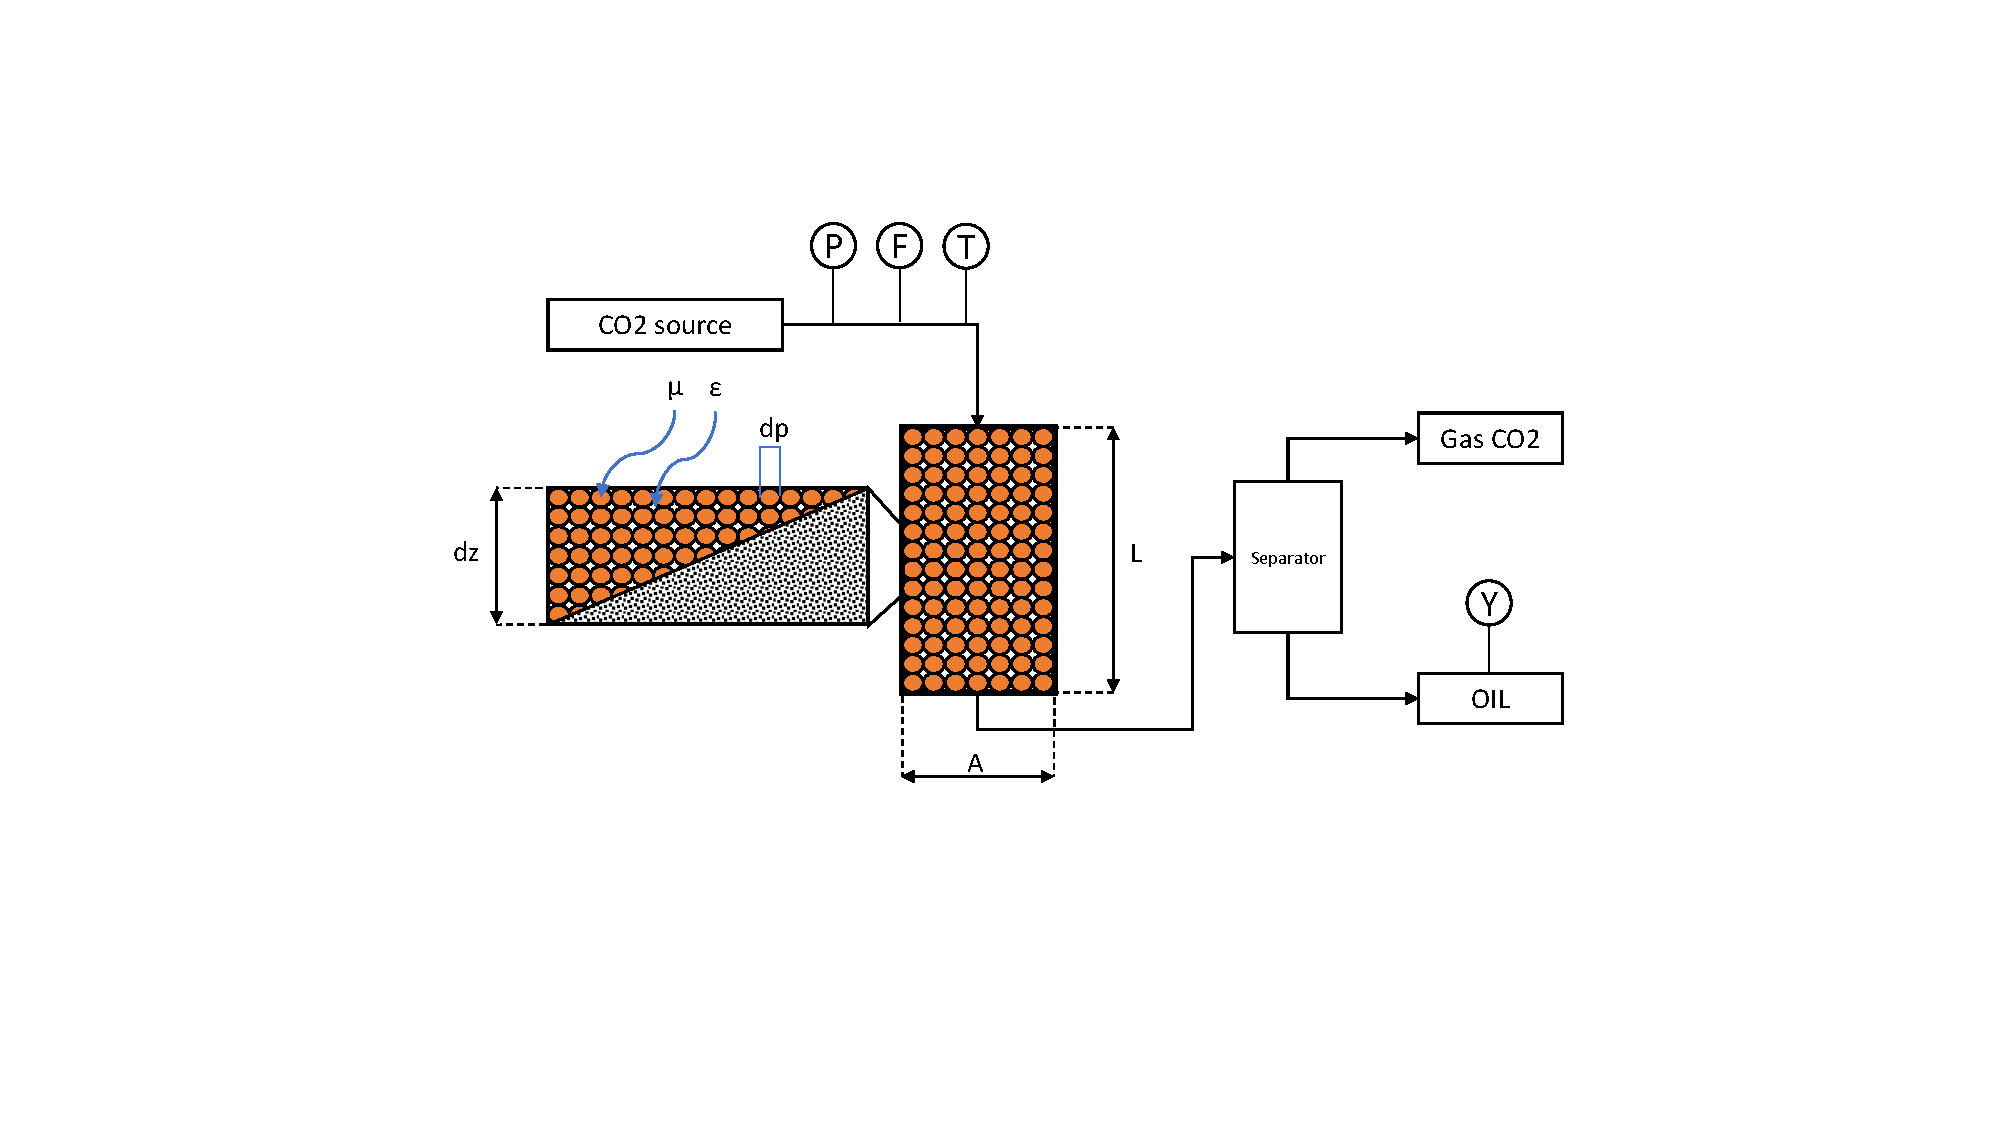
\includegraphics[trim = 4cm 5cm 4cm 3cm,clip,width=\linewidth]{Figures/SFE_Diagram.pdf}
		\caption{Schematic representation of SFE process}
		\label{fig:SFE_drawing}
	\end{figure} 
	\end{frame}
	
	\section{Model description}
	
	\begin{frame}{Model of the extractor}
		\textcolor{red}{control variables},
		\textcolor{blue}{state variables},
		\textcolor{orange}{variables} and
		\textcolor{green}{parameters}\par
		{\footnotesize\begin{align*}
			\intertext{(1) Fluid phase mass balance}
			\cfrac{\partial \textcolor{blue}{c}(t,z)}{\partial t} &=  -\cfrac{1}{ \textcolor{green}{\epsilon A}}\cfrac{\textcolor{red}{F}(t)}{\textcolor{orange}{\rho}(\textcolor{blue}{T}(t,z)\textcolor{red}{P}(t))} \cfrac{\partial \textcolor{blue}{c}(t,z)}{\partial  \textcolor{blue}{z}} 
			+ \textcolor{orange}{D^M_e}(\textcolor{blue}{T}(t,z)\textcolor{red}{P}(t)) \cfrac{\partial^2 \textcolor{blue}{c}(t,z)}{\partial \textcolor{blue}{z^2}} + \cfrac{1-\textcolor{green}{\epsilon}}{\textcolor{green}{\epsilon}} \textcolor{blue}{r_e}(t,z)\\
%		\end{align*}}
		\intertext{(2) Solid phase mass balance}
%		{\scriptsize\begin{align*}
			\cfrac{\partial \textcolor{blue}{q}(t,z)}{\partial t} &= \textcolor{blue}{r_e}(t,z)\\
%		\end{align*}}
		\intertext{(3) Heat balance}
%		{\scriptsize\begin{align*}
			\cfrac{\partial \textcolor{blue}{T}(t,z)}{\partial t} &= -\cfrac{\textcolor{red}{F}(t)}{\textcolor{green}{A}} \cfrac{\textcolor{orange}{C_p}(\textcolor{blue}{T}(t,z)\textcolor{red}{P}(t))}{ [(1-\textcolor{green}{\epsilon})\textcolor{orange}{\rho}(\textcolor{blue}{T}(t,z)\textcolor{red}{P}(t)) \textcolor{orange}{C_p} (\textcolor{blue}{T}(t,z)\textcolor{red}{P}(t)) + \textcolor{green}{ \epsilon \rho_s C_{ps} } ]} \cfrac{\partial \textcolor{blue}{T}(t,z)}{\partial \textcolor{blue}{z}} 
			+  \textcolor{orange}{D^T_e}(\textcolor{blue}{T}(t,z)\textcolor{red}{P}(t)) \cfrac{\partial^2 \textcolor{blue}{T}(t,z)}{\partial \textcolor{blue}{z^2}}\\
%		\end{align*}}
		\\ \intertext{Extraction kinetic}
%		{\scriptsize\begin{align*}
			\textcolor{blue}{r_e}(t,z) &= -\cfrac{\textcolor{orange}{D_i}(\textcolor{blue}{T}(t,z))}{\textcolor{green}{ \mu l^2} }\left(\textcolor{blue}{q}(t,z) - \textcolor{blue}{c}(t,z) \cfrac{\textcolor{green}{\rho_s}}{\textcolor{orange}{k_m}(\textcolor{blue}{T}(t,z))\textcolor{orange}{\rho}(\textcolor{blue}{T}(t,z)\textcolor{red}{P}(t))} \right)\\
%		\end{align*}}
		\intertext{Output function}
%		{\scriptsize\begin{align*}
			\textcolor{blue}{y}(t) &= \textcolor{blue}{g}(x(t)) =\cfrac{\sum\limits_{i=1}^{N_z}  \left(  \textcolor{green}{\cfrac{1}{N_z}} \left(\textcolor{green}{m_0} - \textcolor{blue}{m}_i(t,z) \right) \right) }{\textcolor{green}{m_0}} =  \cfrac{\sum\limits_{i=1}^{N_z}  \left(  \textcolor{green}{\cfrac{V}{N_z}} \left(\textcolor{green}{q_0} - \textcolor{blue}{q}_i(t,z) \right) \right) }{\textcolor{green}{q_0 V}}
		\end{align*}}
	\end{frame}

	\begin{frame}[fragile]{SFE - assumptions}
	\begin{itemize}
		\item One-dimensional model
		\item Plug flow 
		\item No pressure drop
		\item Negligible external diffusion 
		\item Single component
		\item Pseudo-homogeneous thermal properties
		\item Uniformly distribution of the particles
	\end{itemize}
	\end{frame}
	
	\begin{frame}{Model dependencies}
		\par
	{\footnotesize\begin{align*}
			\intertext{(1) Density - Peng-Robinson}
			\textcolor{red}{P}(t) &= \frac{RT}{V_m - b} - \frac{a\alpha}{V_m^2 + 2bV_m - b^2}\\
			\intertext{(2) Solid phase mass balance}
			\textcolor{orange}{C_p}(\textcolor{blue}{T}(t,z)\textcolor{red}{P}(t)) &= Cp_{Ideal} + Cv_{corr} + T\left(\frac{\partial P}{\partial T}\right)_V\left(\frac{\partial V}{\partial T}\right)_P - R\\
			\intertext{(3) Axial diffusion of the mass }
			\textcolor{orange}{D_e^M} (\textcolor{blue}{T}(t,z)\textcolor{red}{P}(t)) &= \cfrac{\textcolor{orange}{u}(\textcolor{blue}{T}(t,z)\textcolor{red}{P}(t)) \textcolor{green}{d_p}}{\textcolor{green}{\epsilon} P_e}\\
			\intertext{(4) Axial diffusion of the heat}
			\textcolor{orange}{D_e^T}\left[\cfrac{m^2}{s}\right] (\textcolor{blue}{T}(t,z)\textcolor{red}{P}(t)) &= \cfrac{\textcolor{orange}{k^T} (\textcolor{blue}{T}(t,z)\textcolor{red}{P}(t))}{\textcolor{orange}{\rho} (\textcolor{blue}{T}(t,z)\textcolor{red}{P}(t)) \textcolor{orange}{C_p} (\textcolor{blue}{T}(t,z)\textcolor{red}{P}(t))}
			\intertext{(5) Internal diffusion}
			\textcolor{orange}{D_i}(\textcolor{blue}{T}(t,z)) \left[\cfrac{m^2}{s}\right] &= \textcolor{green}{D_{i_0}} \exp\left(\cfrac{-\textcolor{green}{EA_{D_i}}}{\textcolor{green}{R} \textcolor{blue}{T}(t,z)}\right) \\
			\intertext{(6) Partition coefficient}
			\textcolor{orange}{k_m}(\textcolor{blue}{T}(t,z))\left[-\right]  &=\textcolor{green}{k_{m_0}} \exp\left(\cfrac{-\textcolor{green}{EA_{k_m}}}{\textcolor{green}{R} \textcolor{blue}{T}(t,z)}\right)
	\end{align*}}
	\end{frame}
	
	\begin{frame}[fragile]{SFE - state-space model}
		\begin{align*}
			\begin{bmatrix}
				\cfrac{\partial c(t,z)}{\partial t}\\
				\cfrac{\partial q(t,z)}{\partial t}\\
				\cfrac{\partial T(t,z)}{\partial t} 
			\end{bmatrix}
			=
			\begin{bmatrix}
				\phi_1 \left( c(t,z),q(t,z),T(t,z); \theta \right)\\
				\phi_2 \left( c(t,z),q(t,z),T(t,z); \theta \right)\\
				\phi_3 \left( c(t,z),q(t,z),T(t,z); \theta \right)
			\end{bmatrix}
			= \phi \left( t,z; \theta \right) &= \cfrac{\partial \chi(t,z)}{\partial t}
		\end{align*}
	\\
	where $\theta$ is a set of parameters present in the model, $\phi$ is a set of functions which correspond to state equations of the model and $\chi$ is the state space model.
	\end{frame}
	
	\begin{frame}[fragile]{SFE - discretization}
		\small{
		\begin{align*}
			\cfrac{d x(t)}{d t} &= 
			\begin{bmatrix}
				\cfrac{d c_1(t)}{d t} 	  \\
				\vdots					  \\
				\cfrac{d c_{N_z}(t)}{d t} \\
				\cfrac{d q_1(t)}{d t} 	  \\
				\vdots					  \\
				\cfrac{d q_{N_z}(t)}{d t} \\
				\cfrac{d T_1(t)}{d t} 	  \\
				\vdots 					  \\
				\cfrac{d T_{N_z}(t)}{d t}
			\end{bmatrix}
			=
			\begin{bmatrix}
				F_1 \left( c(t),q(t),T(t); p \right)\\ 
				\vdots\\ 
				F_{N_z} \left( c(t),q(t),T(t); p \right)\\ \\
				F_{N_z+1} \left( c(t),q(t),T(t); p \right)\\
				\vdots\\
				F_{2N_z} \left( c(t),q(t),T(t); p \right)\\ \\
				F_{2N_z+1} \left( c(t),q(t),T(t); p \right) \\
				\vdots\\
				F_{3N_z} \left( c(t),q(t),T(t); p \right)
			\end{bmatrix}
			= F \left( t; p \right)
		\end{align*} }\\
		where $x \in \mathbb{R}^{N_x = 3N_z} $ and $p \in \mathbb{R}^{N_p =  N_{\theta} + N_u } $
	\end{frame}
	
	\section{Sensitivity Analysis}
	
	\begin{frame}[fragile]{Sensitivity Analysis}
		Local derivative-based methods involve taking the partial derivative of the output with respect to an input parameter. In sensitivity analysis the original system of equations is solved simultaneously with $\cfrac{\partial \textcolor{blue}{F}(x(t);p)}{\partial p}$, where $p$ is a vector of all the parameters and the control variables.
	\end{frame}

	\begin{frame}[fragile]{Sensitivity Analysis}
		\small{
		\begin{align*}
			Z &= \cfrac{\partial \textcolor{blue}{x}(t,p)}{\partial \textcolor{green}{p}} \nonumber \\
			\dot{Z}  &= \cfrac{\partial \textcolor{blue}{Z}(t,p)}{\partial t} = \cfrac{\partial }{\partial t} \left( \cfrac{\partial \textcolor{blue}{x}(t,p)}{\partial p} \right) = \cfrac{\partial }{\partial p} \left( \cfrac{\partial \textcolor{blue}{x}(t,p)}{\partial t} \right) = \cfrac{\partial \textcolor{blue}{F}(x(t);p)}{\partial p} \\
			\cfrac{d \textcolor{blue}{F}(x(t);p)}{d p} &=  \cfrac{\partial F(x(t);p)}{\partial x(t)} \cfrac{\partial x(t)}{\partial p} + \cfrac{\partial F(x(t);p)}{\partial p}  \\
			& = J_x(x(t);p)S(x(t);p) + J_p(x(t);p)
		\end{align*}
		}
		\tiny{
		\[
		\framebox[1.2cm]{\claps{\raisebox{0pt}[1.0cm][1.0cm]{$\mat {\cfrac{d F(x(t);p)}{dp}} $}}\subdims{-1.5cm} {N_x} {N_p}} =
		\framebox[2.0cm]{\claps{\raisebox{0pt}[1.0cm][1.0cm]{$\mat J_x$}}\subdims{-1.5cm} {N_x} {N_x}} \ 
		\framebox[1.2cm]{\claps{\raisebox{0pt}[1.0cm][1.0cm]{$\mat S$}}  \subdims{-1.5cm} {N_x} {N_p}} + 
		\framebox[1.2cm]{\claps{\raisebox{0pt}[1.0cm][1.0cm]{$\mat J_p$}}\subdims{-1.5cm} {N_x} {N_p}}
		\]}
	
	\end{frame}

	\begin{frame}[fragile]{Sensitivity Analysis}
		\tiny{\begin{align*}
			\begin{split}
				\cfrac{d F(x(t);p)}{dp} &=\left(\begin{array}{cccc}
					\cfrac{\partial F_{1}(x(t);p)}{\partial x_{1}(t)} & \cfrac{\partial F_{1}(x(t);p)}{\partial x_{2}(t)} & \cdots & \cfrac{\partial F_{1}(x(t);p)}{\partial x_{N_x}(t)}\\
					\cfrac{\partial F_{2}(x(t);p)}{\partial x_{1}(t)} & \cfrac{\partial F_{2}(x(t);p)}{\partial x_{2}(t)} & \cdots & \cfrac{\partial F_{2}(x(t);p)}{\partial x_{N_x}(t)}\\
					\vdots & \vdots & \ddots & \vdots\\ 
					\cfrac{\partial F_{N_x}(x(t);p)}{\partial x_{1}(t)} & \cfrac{\partial F_{N_x}(x(t);p)}{\partial x_{2}(t)} & \cdots & \cfrac{\partial F_{N_x}(x(t);p)}{\partial x_{N_x}(t)}
				\end{array}\right)
			\begin{pmatrix}
				\cfrac{d x_{1}(t)}{d p_{1}} 	& \cfrac{d x_{1}(t)}{d p_{2}}     & \cdots & \cfrac{d x_{1}(t)}{d p_{N_p}}\\
				\cfrac{d x_{2}(t)}{d p_{1}}		& \cfrac{d x_{2}(t)}{d p_{2}}     & \cdots & \cfrac{d x_{2}(t)}{d p_{N_p}}\\
				\vdots					 	    & \vdots 					   	  & \ddots & \vdots\\
				\cfrac{d x_{N_x}(t)}{d p_{1}} 	& \cfrac{d x_{N_x}(t)}{d p_{2}}   & \cdots & \cfrac{d x_{N_x}(t)}{d p_{N_p}}
			\end{pmatrix}
		 + \\
	   & + \left(\begin{array}{cccc}
				\cfrac{\partial F_{1}(x(t);p)}{\partial p_{1}} & \cfrac{\partial F_{1}(x(t);p)}{\partial p_{2}} & \cdots & \cfrac{\partial F_{1}(x(t);p)}{\partial p_{N_p}}\\
				\cfrac{\partial F_{2}(x(t);p)}{\partial p_{1}} & \cfrac{\partial F_{2}(x(t);p)}{\partial p_{2}} & \cdots & \cfrac{\partial F_{2}(x(t);p)}{\partial p_{N_p}}\\
				\vdots & \vdots & \ddots & \vdots\\
				\cfrac{\partial F_{N_x}(x(t);p)}{\partial p_{1}} & \cfrac{\partial F_{N_x}(x(t);p)}{\partial p_{2}} & \cdots & \cfrac{\partial F_{N_x}(x(t);p)}{\partial p_{N_p}}
			\end{array}\right)
	\end{split}\end{align*}
	}
	\end{frame}

	\begin{frame}[fragile]{Sensitivity Analysis}
		The$F(x(t);p)$ is augmented with sensitivity equations and denoted as \textbf{F}$\left(x(t);p\right)$. The size of \textbf{F}$\left(x(t);p\right)$ is equal to $N_s = N_x(N_p + 1)$.
		\small{
		\begin{align*}
			\textbf{F}\left(x(t);p\right) = 
			\begin{bmatrix}
				F(x(t);p)\\
				J_x(x(t);p)S(x(t);p) + J_p(x(t);p)
			\end{bmatrix}
		\end{align*} } \\
		The initial conditions are described as
		\small{
		\begin{align*}
			\textbf{F}\left(x(t_0);p\right)  = 
			\begin{bmatrix} x(t_0),			& 
				\cfrac{ \text{d}x(t_0) }{ dp_1 },		& 
				\cdots,					 	&
				\cfrac{ dx(t_0) }{ dp_{N_p} } 
			\end{bmatrix}^T
		\end{align*} }
	\end{frame}

	\begin{frame}[fragile]{Sensitivity Analysis}

		\footnotesize{\begin{align*}
		\textcolor{blue}{y}(t) &= \textcolor{blue}{g}(x(t)) =\cfrac{\sum\limits_{i=1}^{N_z}  \left(  \textcolor{green}{\cfrac{1}{N_z}} \left(\textcolor{green}{m_0} - \textcolor{blue}{m}_i(t,z) \right) \right) }{\textcolor{green}{m_0}} =  \cfrac{\sum\limits_{i=1}^{N_z}  \left(  \textcolor{green}{\cfrac{V}{N_z}} \left(\textcolor{green}{q_0} - \textcolor{blue}{q}_i(t,z) \right) \right) }{\textcolor{green}{q_0 V}}\\ 
		\end{align*}}
		By taking a total derivative of $y(t)$ with respect to $p$, the new sensitivity equation can found.\\
		\footnotesize{\begin{align*}
		\cfrac{d y(t)}{dp} &= \cfrac{d g(x(t))}{dp} = \cfrac{\partial g(x(t))}{\partial x(t)} \cfrac{\partial x(t)}{\partial p} + \cfrac{\partial g(x(t))}{\partial p}\\
		\cfrac{\partial g(x(t))}{\partial p} &= \cfrac{\partial g(x(t))}{\partial x(t)} \cfrac{\partial x(t)}{\partial p} + 0 = \cfrac{\partial g(x(t))}{\partial x(t)}  S(x(t);p) = \\
		\begin{split}
				&\left(\begin{array}{cccc}
					\cfrac{\partial g_{1}(x(t))}{\partial x_{1}} & \cfrac{\partial g_{1}(x(t))}{\partial x_{2}} & \cdots & \cfrac{\partial g_{1}(x(t))}{\partial x_{N_x}}\\
					\cfrac{\partial g_{2}(x(t))}{\partial x_{1}} & \cfrac{\partial g_{2}(x(t))}{\partial x_{2}} & \cdots & \cfrac{\partial g_{2}(x(t))}{\partial x_{N_x}}\\
					\vdots & \vdots & \ddots & \vdots\\
					\cfrac{\partial g_{N_g}(x(t))}{\partial x_{1}} & \cfrac{\partial g_{N_g}(x(t))}{\partial x_{2}} & \cdots & \cfrac{\partial g_{N_g}(x(t))}{\partial x_{N_x}}
				\end{array}\right)
				\left(\begin{array}{cccc}
					s_{({1,1})} & s_{({1,2})} & \cdots & s_{({1,N_p})}\\
					s_{({2,1})} & s_{({2,2})} & \cdots & s_{({2,N_p})}\\
					\vdots & \vdots & \ddots & \vdots\\
					s_{({N_x,1})} & s_{({N_x,2})} & \cdots & s_{({N_x,N_p})}\\
				\end{array}\right)
		\end{split}
	\end{align*}}
	\end{frame}
	
	\begin{frame}[fragile]{Sensitivity Analysis}
		Because the output function returns only one value, the equation becomes
		\footnotesize{\begin{align*}\begin{split}
				& \left( \cfrac{\partial y(x(t))}{\partial p_{1}}, \cfrac{\partial y(x(t))}{\partial p_{2}}, \cdots, \cfrac{\partial y(x(t))}{\partial p_{N_p}} \right) = \\
				& =\left( \cfrac{\partial g(x(t))}{\partial x_{1}}, \cfrac{\partial g(x(t))}{\partial x_{2}}, \cdots, \cfrac{\partial g(x(t))}{\partial x_{N_x}} \right)
				\left(\begin{array}{cccc}
					s_{({1,1})} & s_{({1,2})} & \cdots & s_{({1,N_p})}\\
					s_{({2,1})} & s_{({2,2})} & \cdots & s_{({2,N_p})}\\
					\vdots & \vdots & \ddots & \vdots\\
					s_{({N_x,1})} & s_{({N_x,2})} & \cdots & s_{({N_x,N_p})}
				\end{array}\right)
		\end{split}\end{align*}}
	
		\tiny{
		\[
		\framebox[1.5cm]{\claps{\raisebox{0pt}[0.3cm][0.3cm]{$\mat {\cfrac{d g(x(t))}{dp} } $}}		\subdims{-1.7cm} {1} {N_p}} =
		\framebox[2.5cm]{\claps{\raisebox{0pt}[0.3cm][0.3cm]{$\mat {\cfrac{d g(x(t))}{d x(t)} } $}} \subdims{-1.7cm} {1} {N_x}} \ 
		\framebox[1.5cm]{\claps{\raisebox{0pt}[1.25cm][1.25cm]{$\mat S$}}  							\subdims{-1.7cm} {N_x} {N_p}}
		\]}
	
	\end{frame}

	\section{Results}
	
	\begin{frame}[fragile]{Results of the simulation}
	\centering Product: CARQUEJA essential oil
	\begin{table}[!hbt]
		\centering
		\begin{tabular}{ |c|c|c|c|c|c|c|c|c| } 
			\hline
			Ref& $F[kg/hr]$ & $T_{Inlet} [C]$ & $T_{extractor} [C]$ & $P [bar]$ & $c [kg/m^3]$ & $q [kg/m^3]$ \\ \hline
			Vargas & 0.035      & 50              & 50		             & 90  	     & 0 		    & 27 		   \\ \hline
		\end{tabular}
		\caption{Initial conditions}
	\end{table}					
	\begin{columns}[t]
		\column{.5\textwidth}
		\centering
		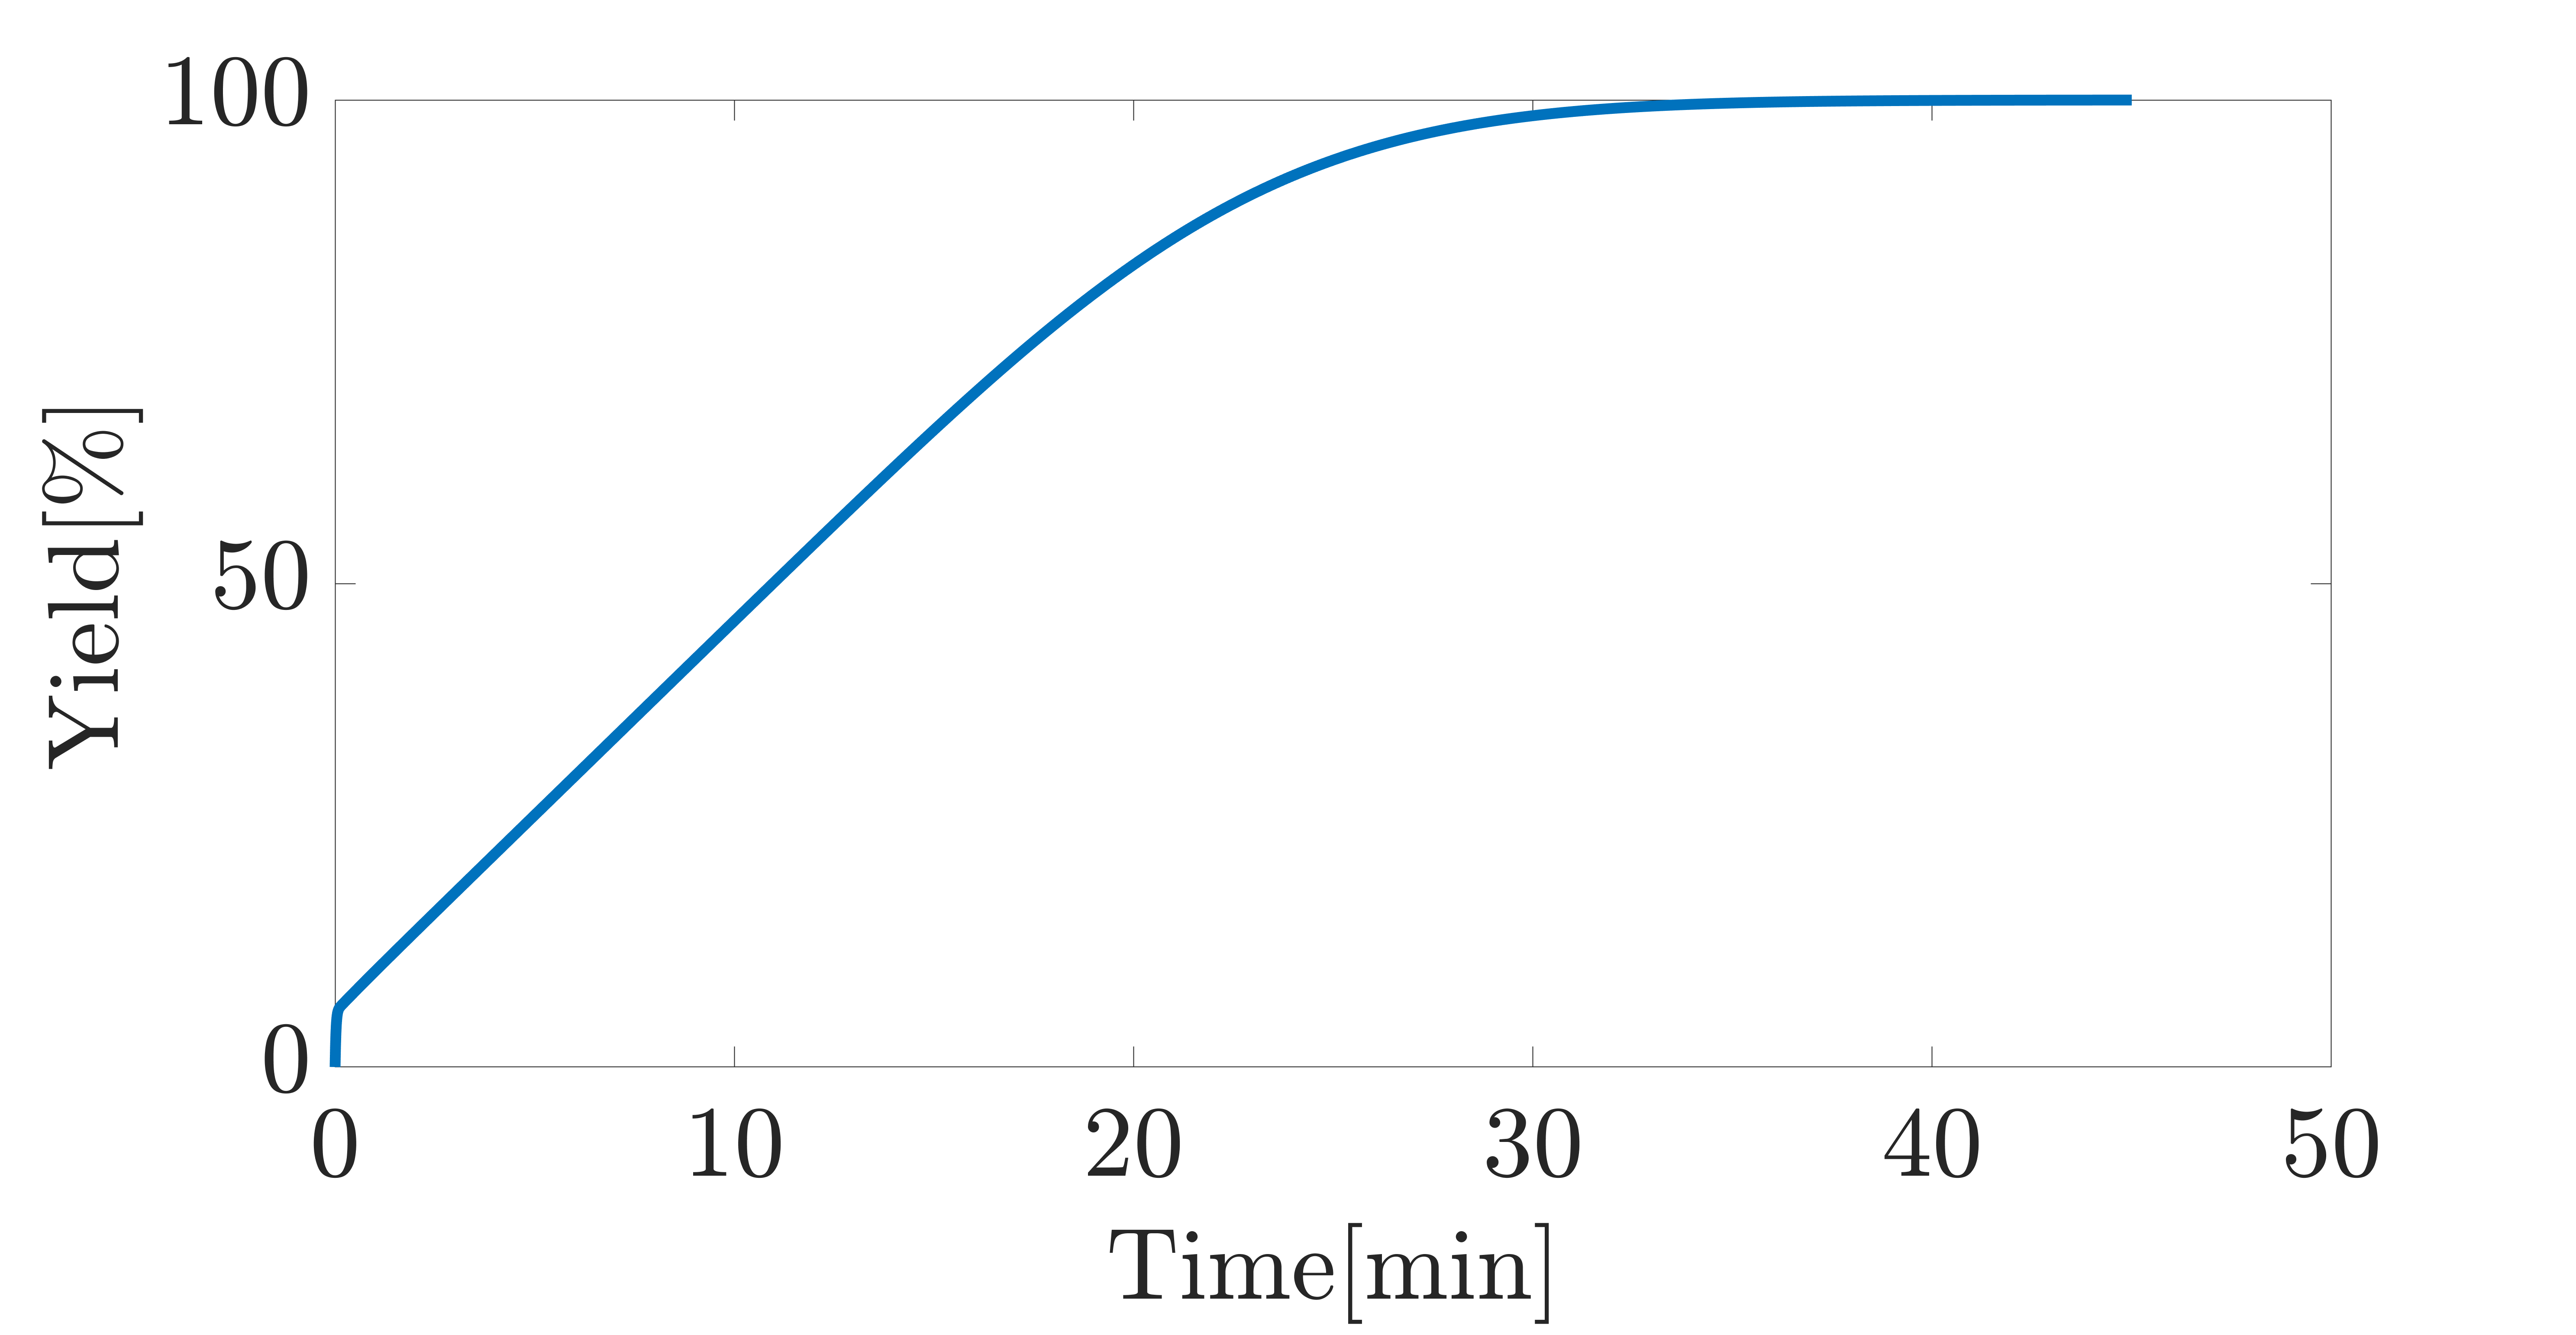
\includegraphics[width=5.5cm,height=2.5cm]{Figures/Sensitivity/Yield.png}\\
		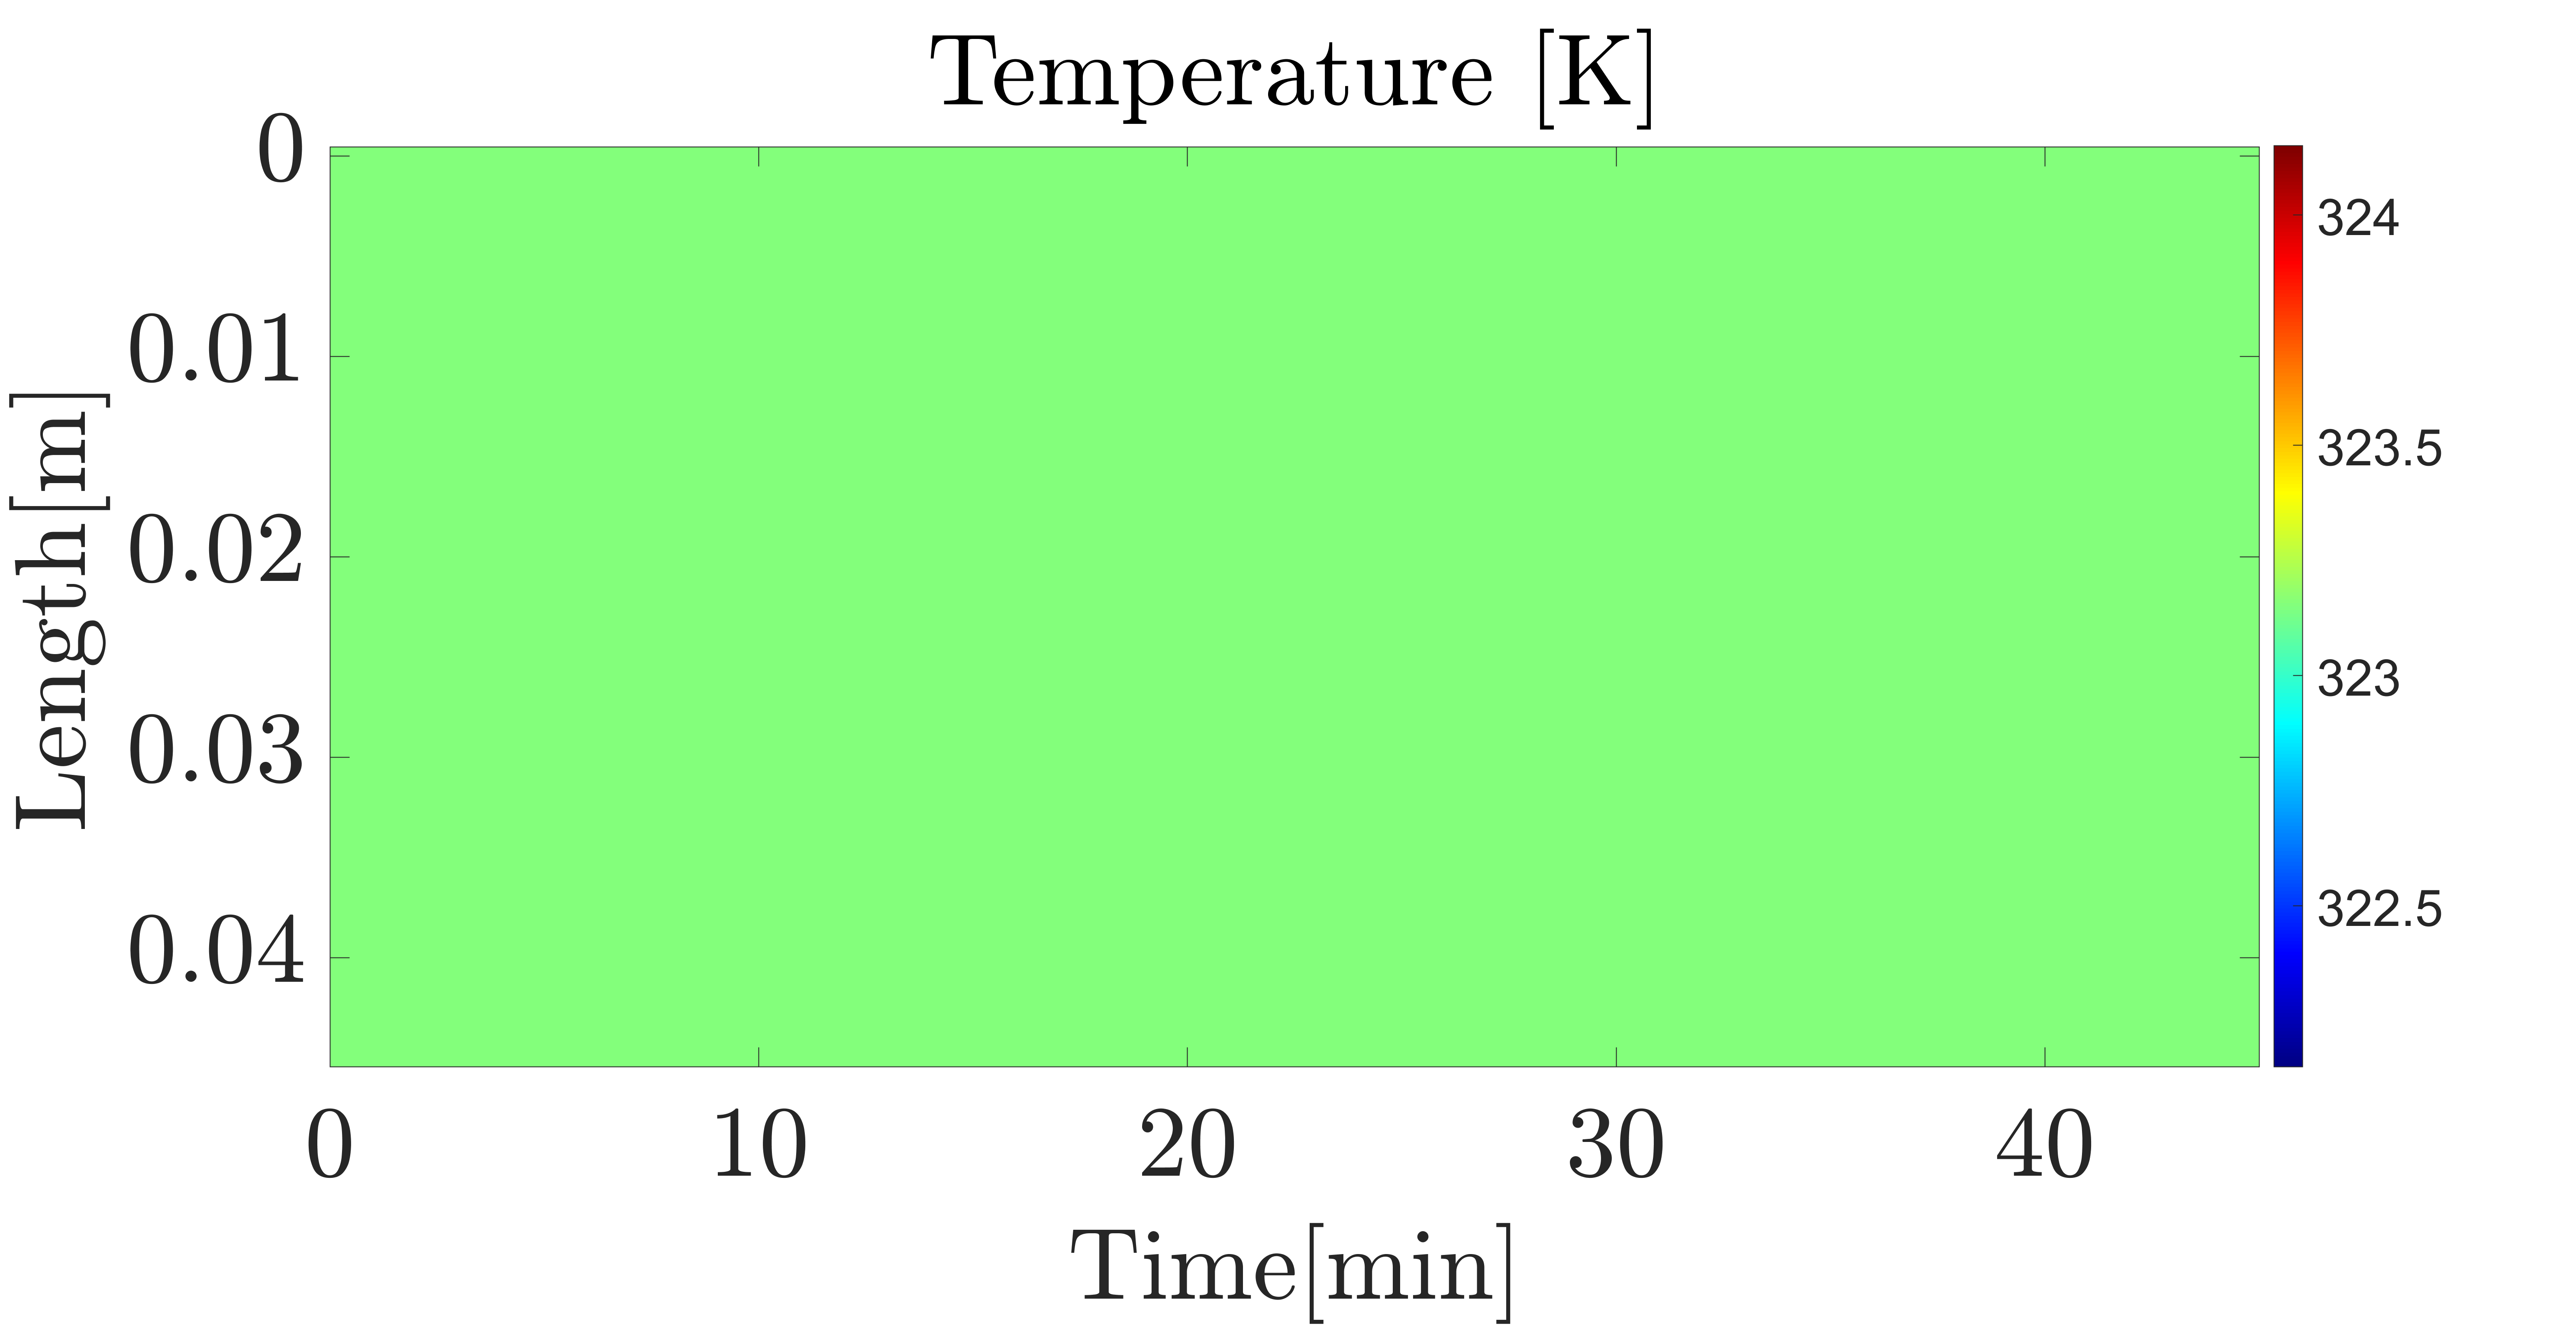
\includegraphics[width=5.5cm,height=2.5cm]{Figures/Sensitivity/Temperature.png}
		\column{.5\textwidth}
		\centering
		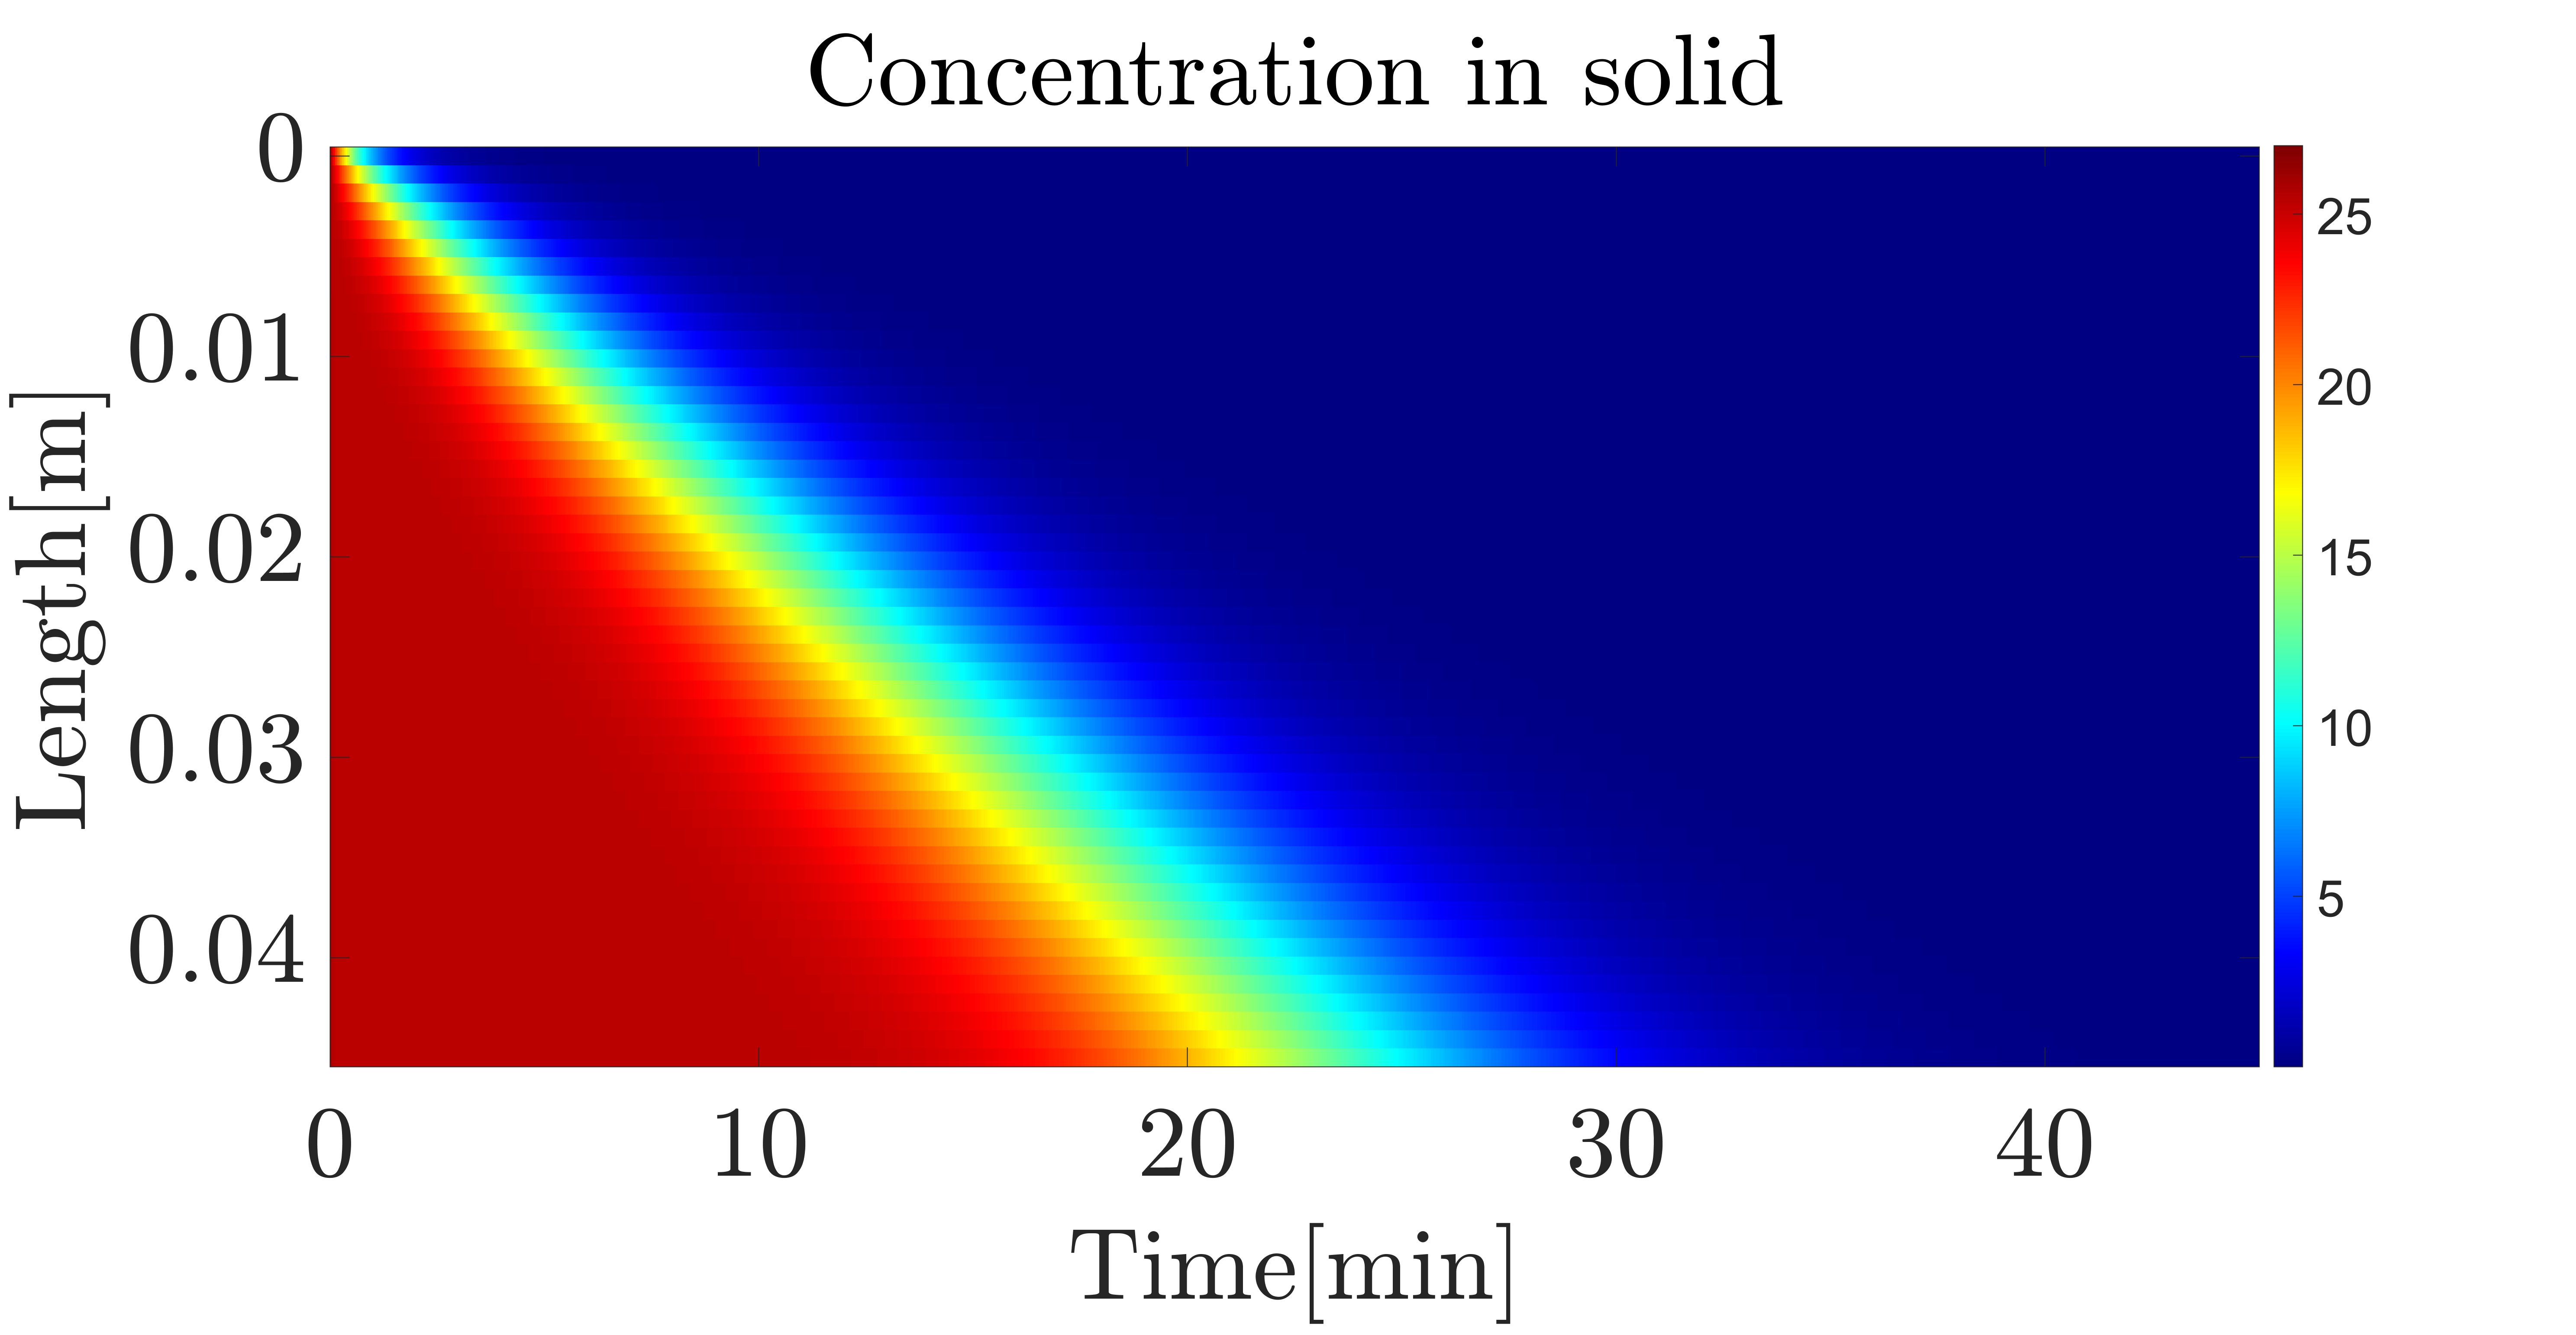
\includegraphics[width=5.5cm,height=2.5cm]{Figures/Sensitivity/ConcentrationSolid.png}\\
		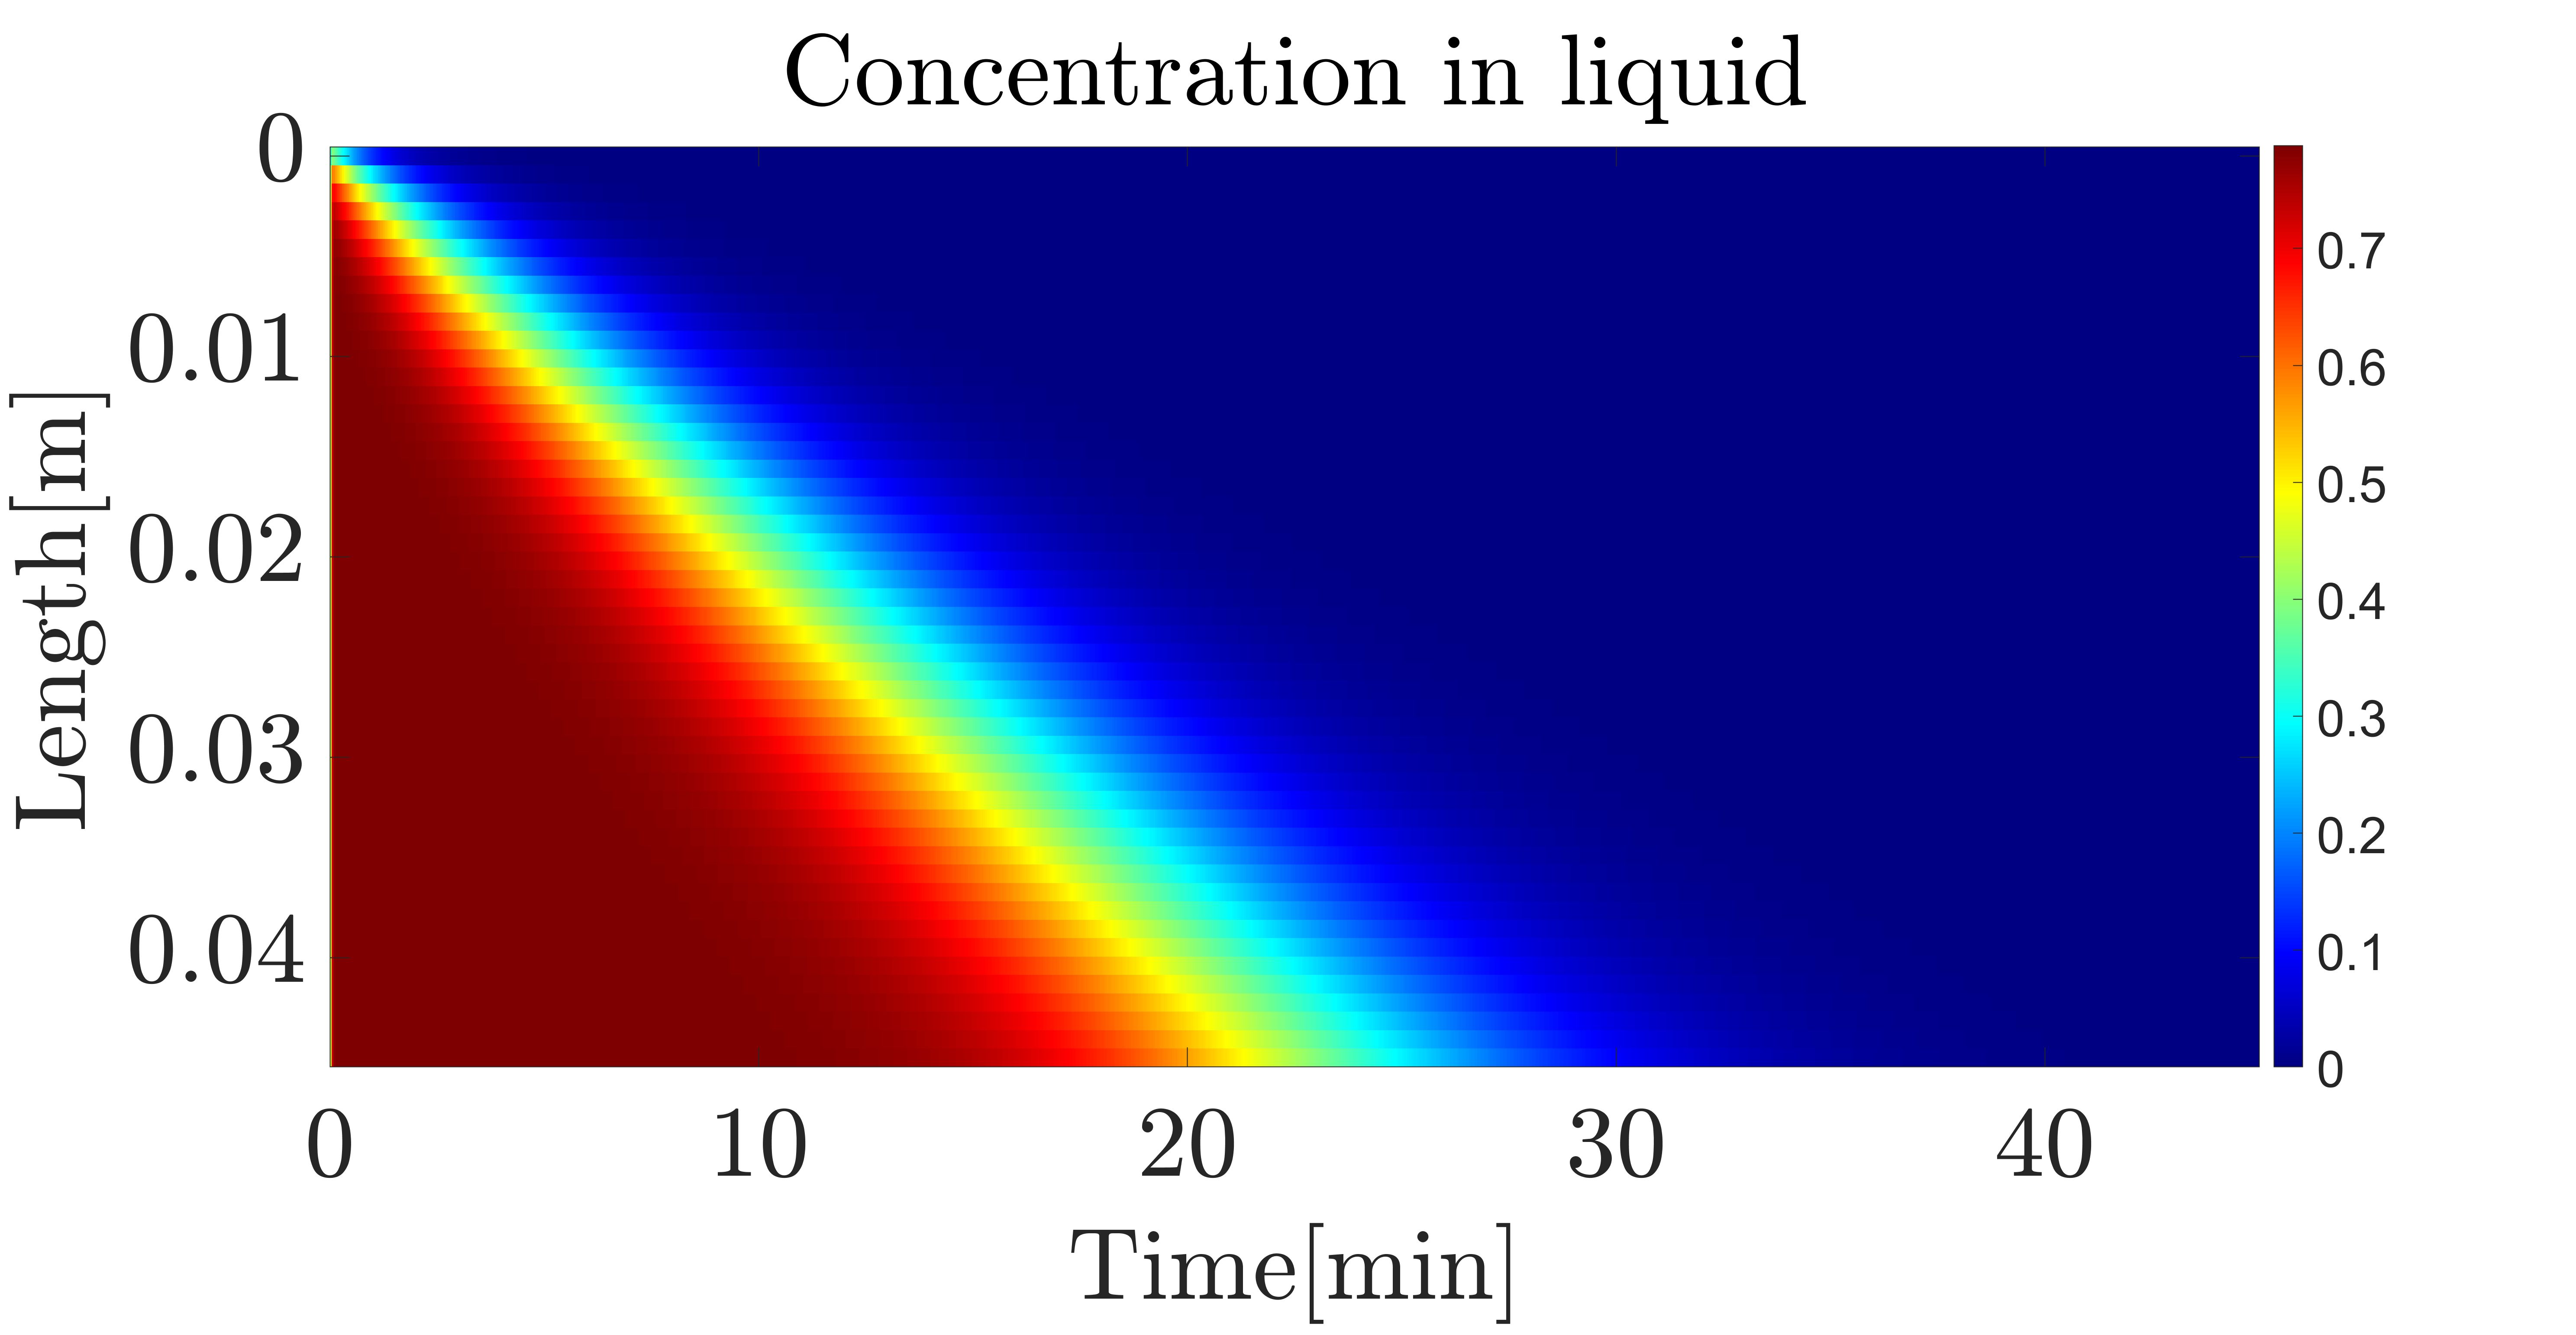
\includegraphics[width=5.5cm,height=2.5cm]{Figures/Sensitivity/ConcentrationLiquid.png}
	\end{columns}
	\end{frame}

	\begin{frame}[fragile]{Sensitivity Analysis - Pressure}
		\tiny{
			\begin{align*}
				\cfrac{\partial \textcolor{blue}{c}(t,z)}{\partial t} &=  -\cfrac{F(t)}{\epsilon A\rho(T(t,z)\textcolor{red}{P}(t))} \cfrac{\partial c(t,z)}{\partial z} 
				+ D^M_e(T(t,z)\textcolor{red}{P}(t)) \cfrac{\partial^2 c(t,z)}{\partial z^2} + \cfrac{1-\epsilon}{\epsilon} \cfrac{D_i(T(t,z))}{\mu l^2 }\left(q(t,z) - \cfrac{c(t,z)\rho_s}{k_m(T(t,z))\rho(T(t,z)\textcolor{red}{P}(t))} \right)\\
				\cfrac{\partial \textcolor{blue}{q}(t,z)}{\partial t} &= -\cfrac{D_i(T(t,z))}{\mu l^2 }\left(q(t,z) - c(t,z) \cfrac{\rho_s}{k_m(T(t,z))\rho(T(t,z)\textcolor{red}{P}(t))} \right)\\
				\cfrac{\partial \textcolor{blue}{T}(t,z)}{\partial t} &= -\cfrac{F(t)}{A} \cfrac{C_p(T(t,z)\textcolor{red}{P}(t))}{ [(1-\epsilon)\rho(T(t,z)\textcolor{red}{P}(t)) C_p(T(t,z)\textcolor{red}{P}(t)) + \epsilon \rho_s C_{ps} ]} \cfrac{\partial T(t,z)}{\partial z} 
				+ D^T_e(T(t,z)\textcolor{red}{P}(t)) \cfrac{\partial^2 T(t,z)}{\partial z^2}
		\end{align*}}
		\begin{columns}[t]
			\column{.5\textwidth}
			\centering
			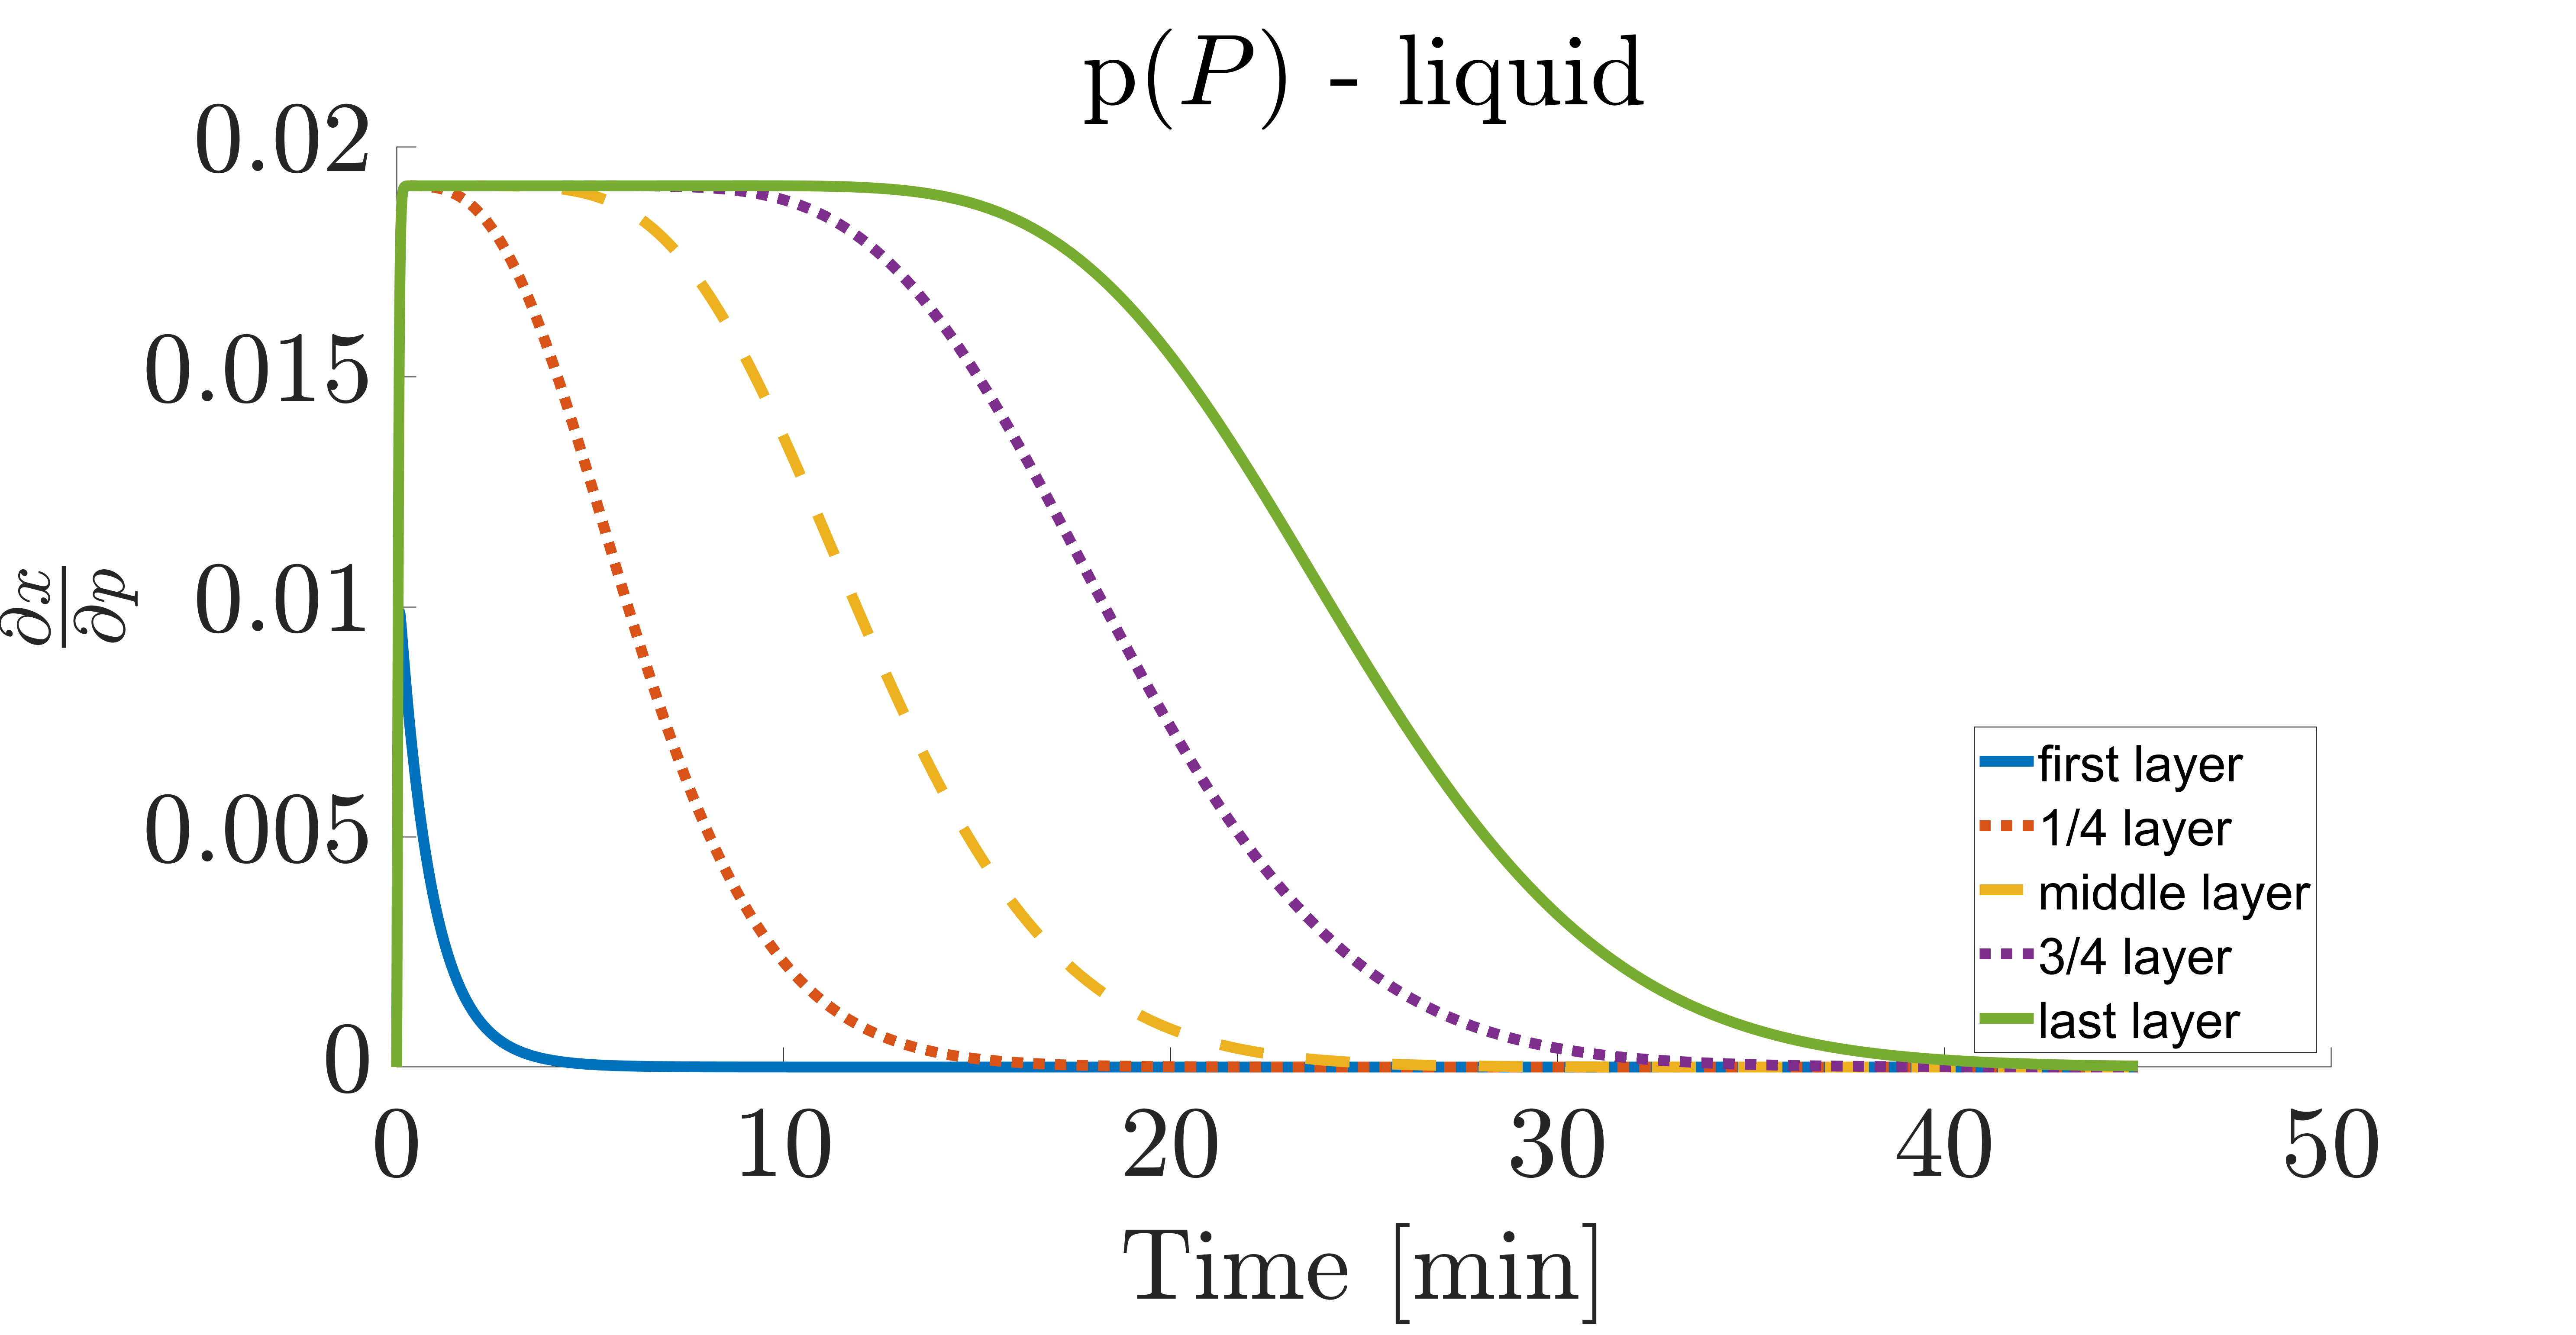
\includegraphics[width=5.5cm,height=2.5cm]{Figures/Sensitivity/Plots/2_SS_R_P.png}\\
			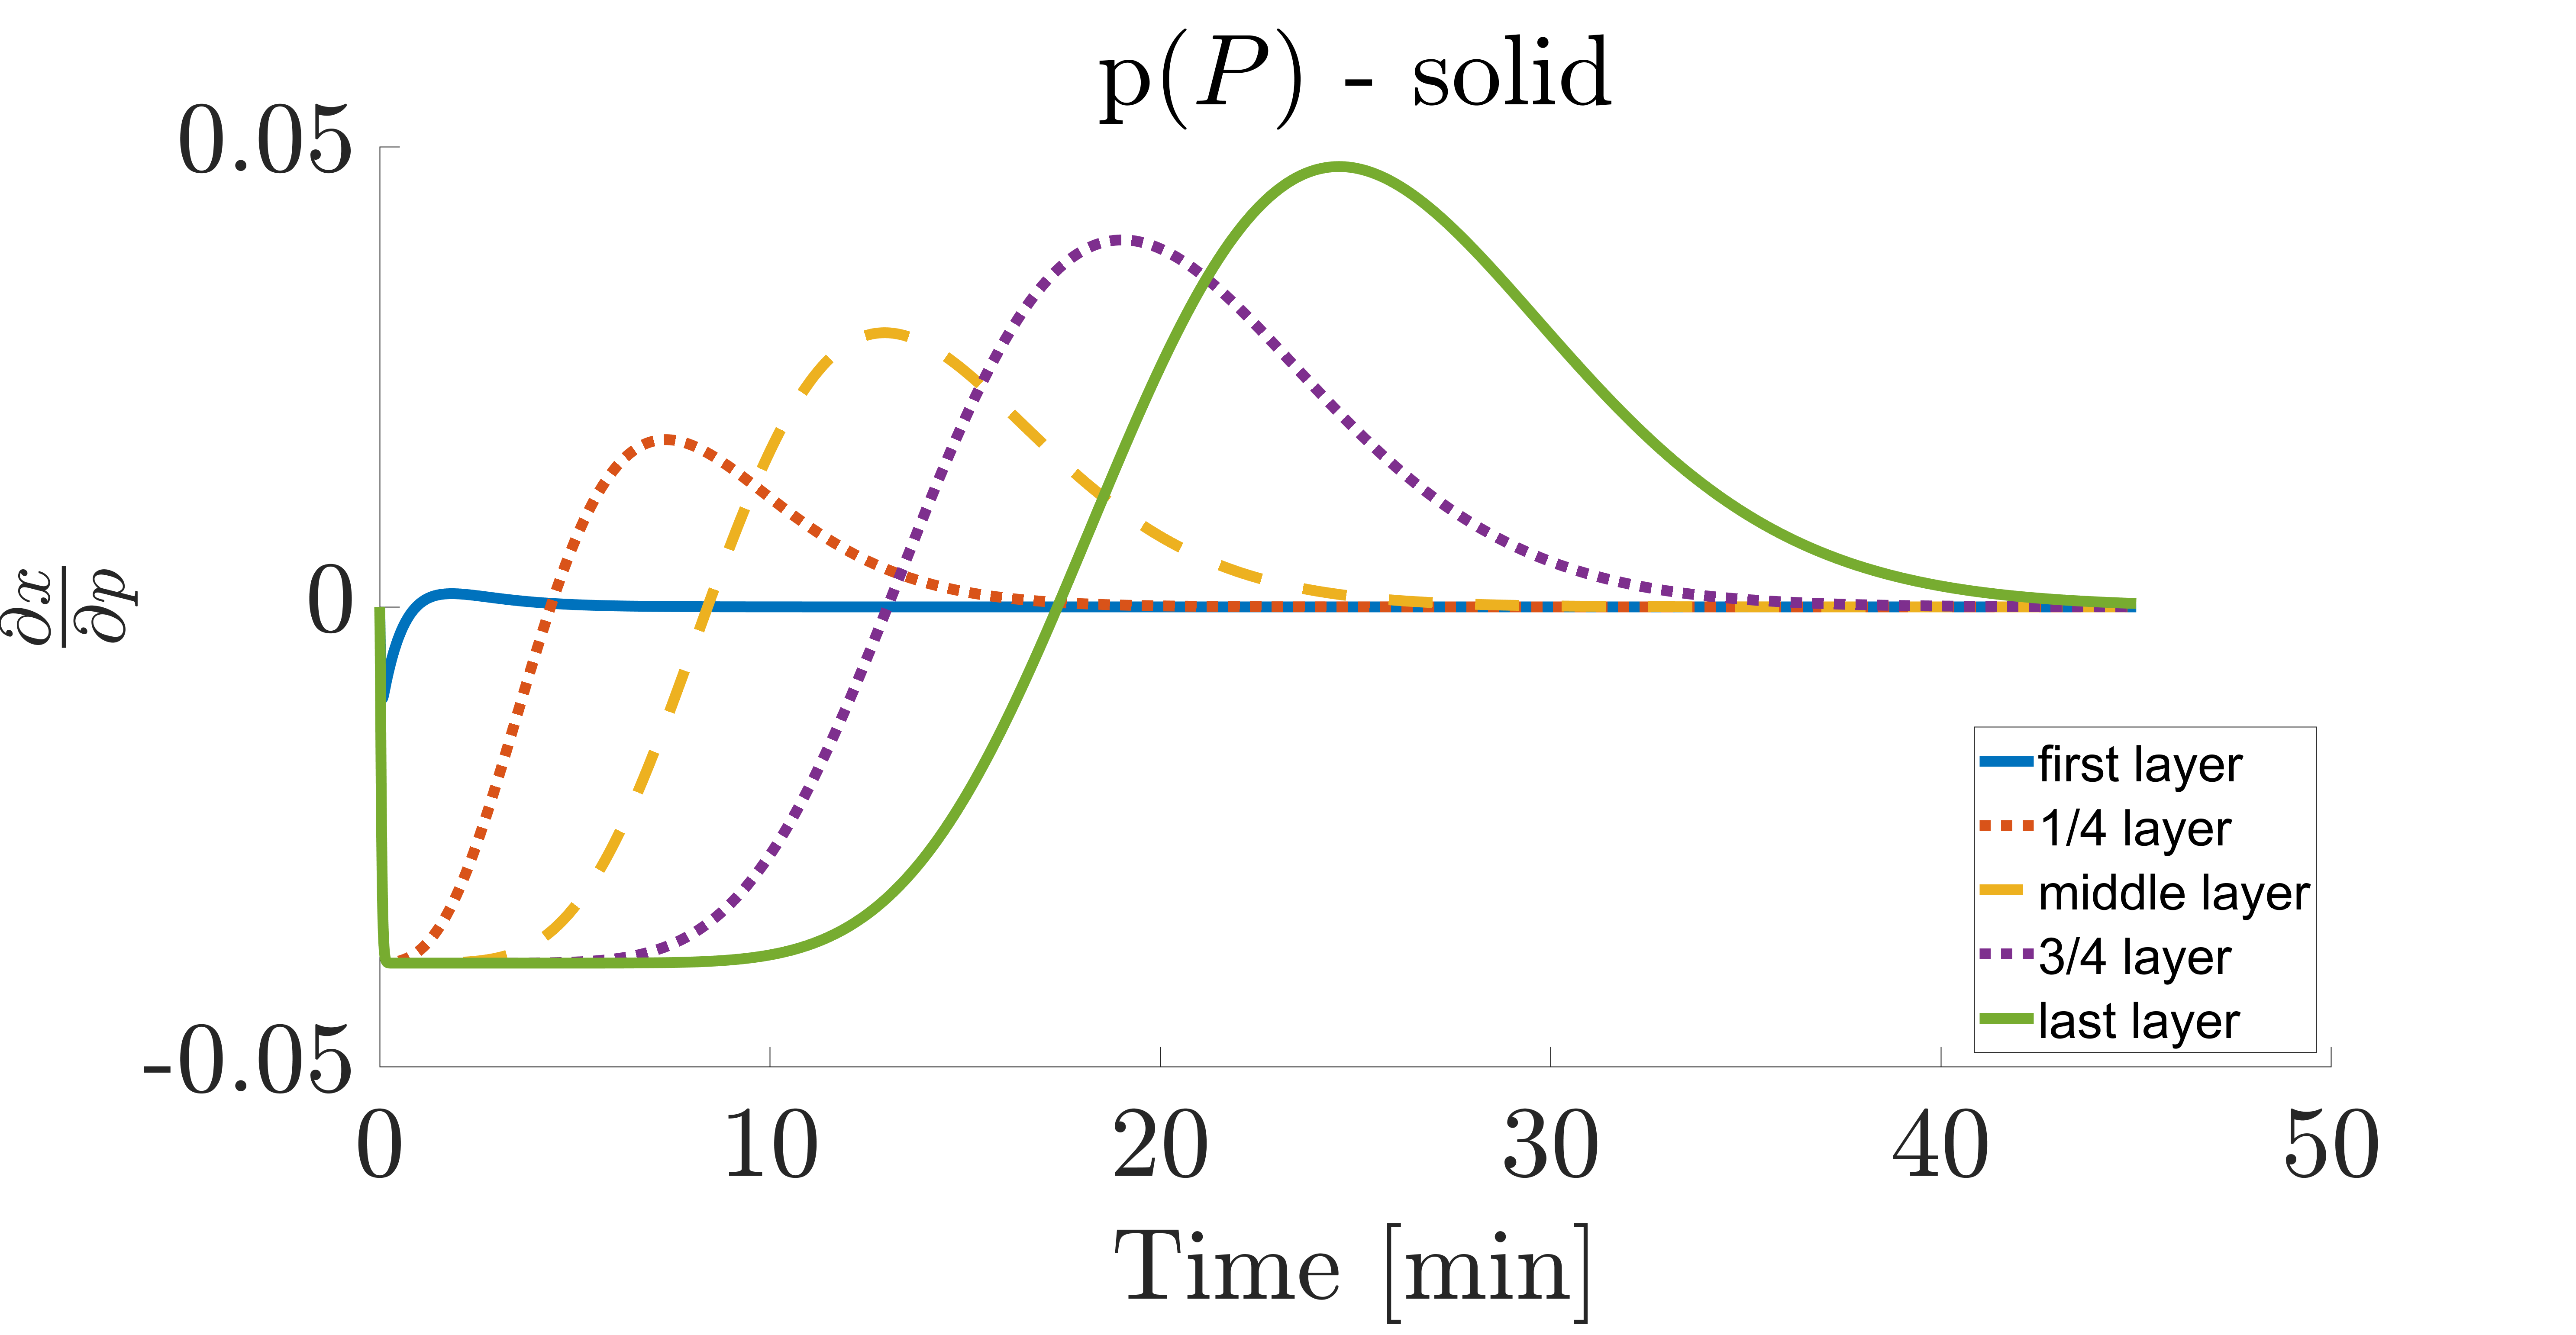
\includegraphics[width=5.5cm,height=2.5cm]{Figures/Sensitivity/Plots/3_SS_R_P.png}
			\column{.5\textwidth}
			\centering
			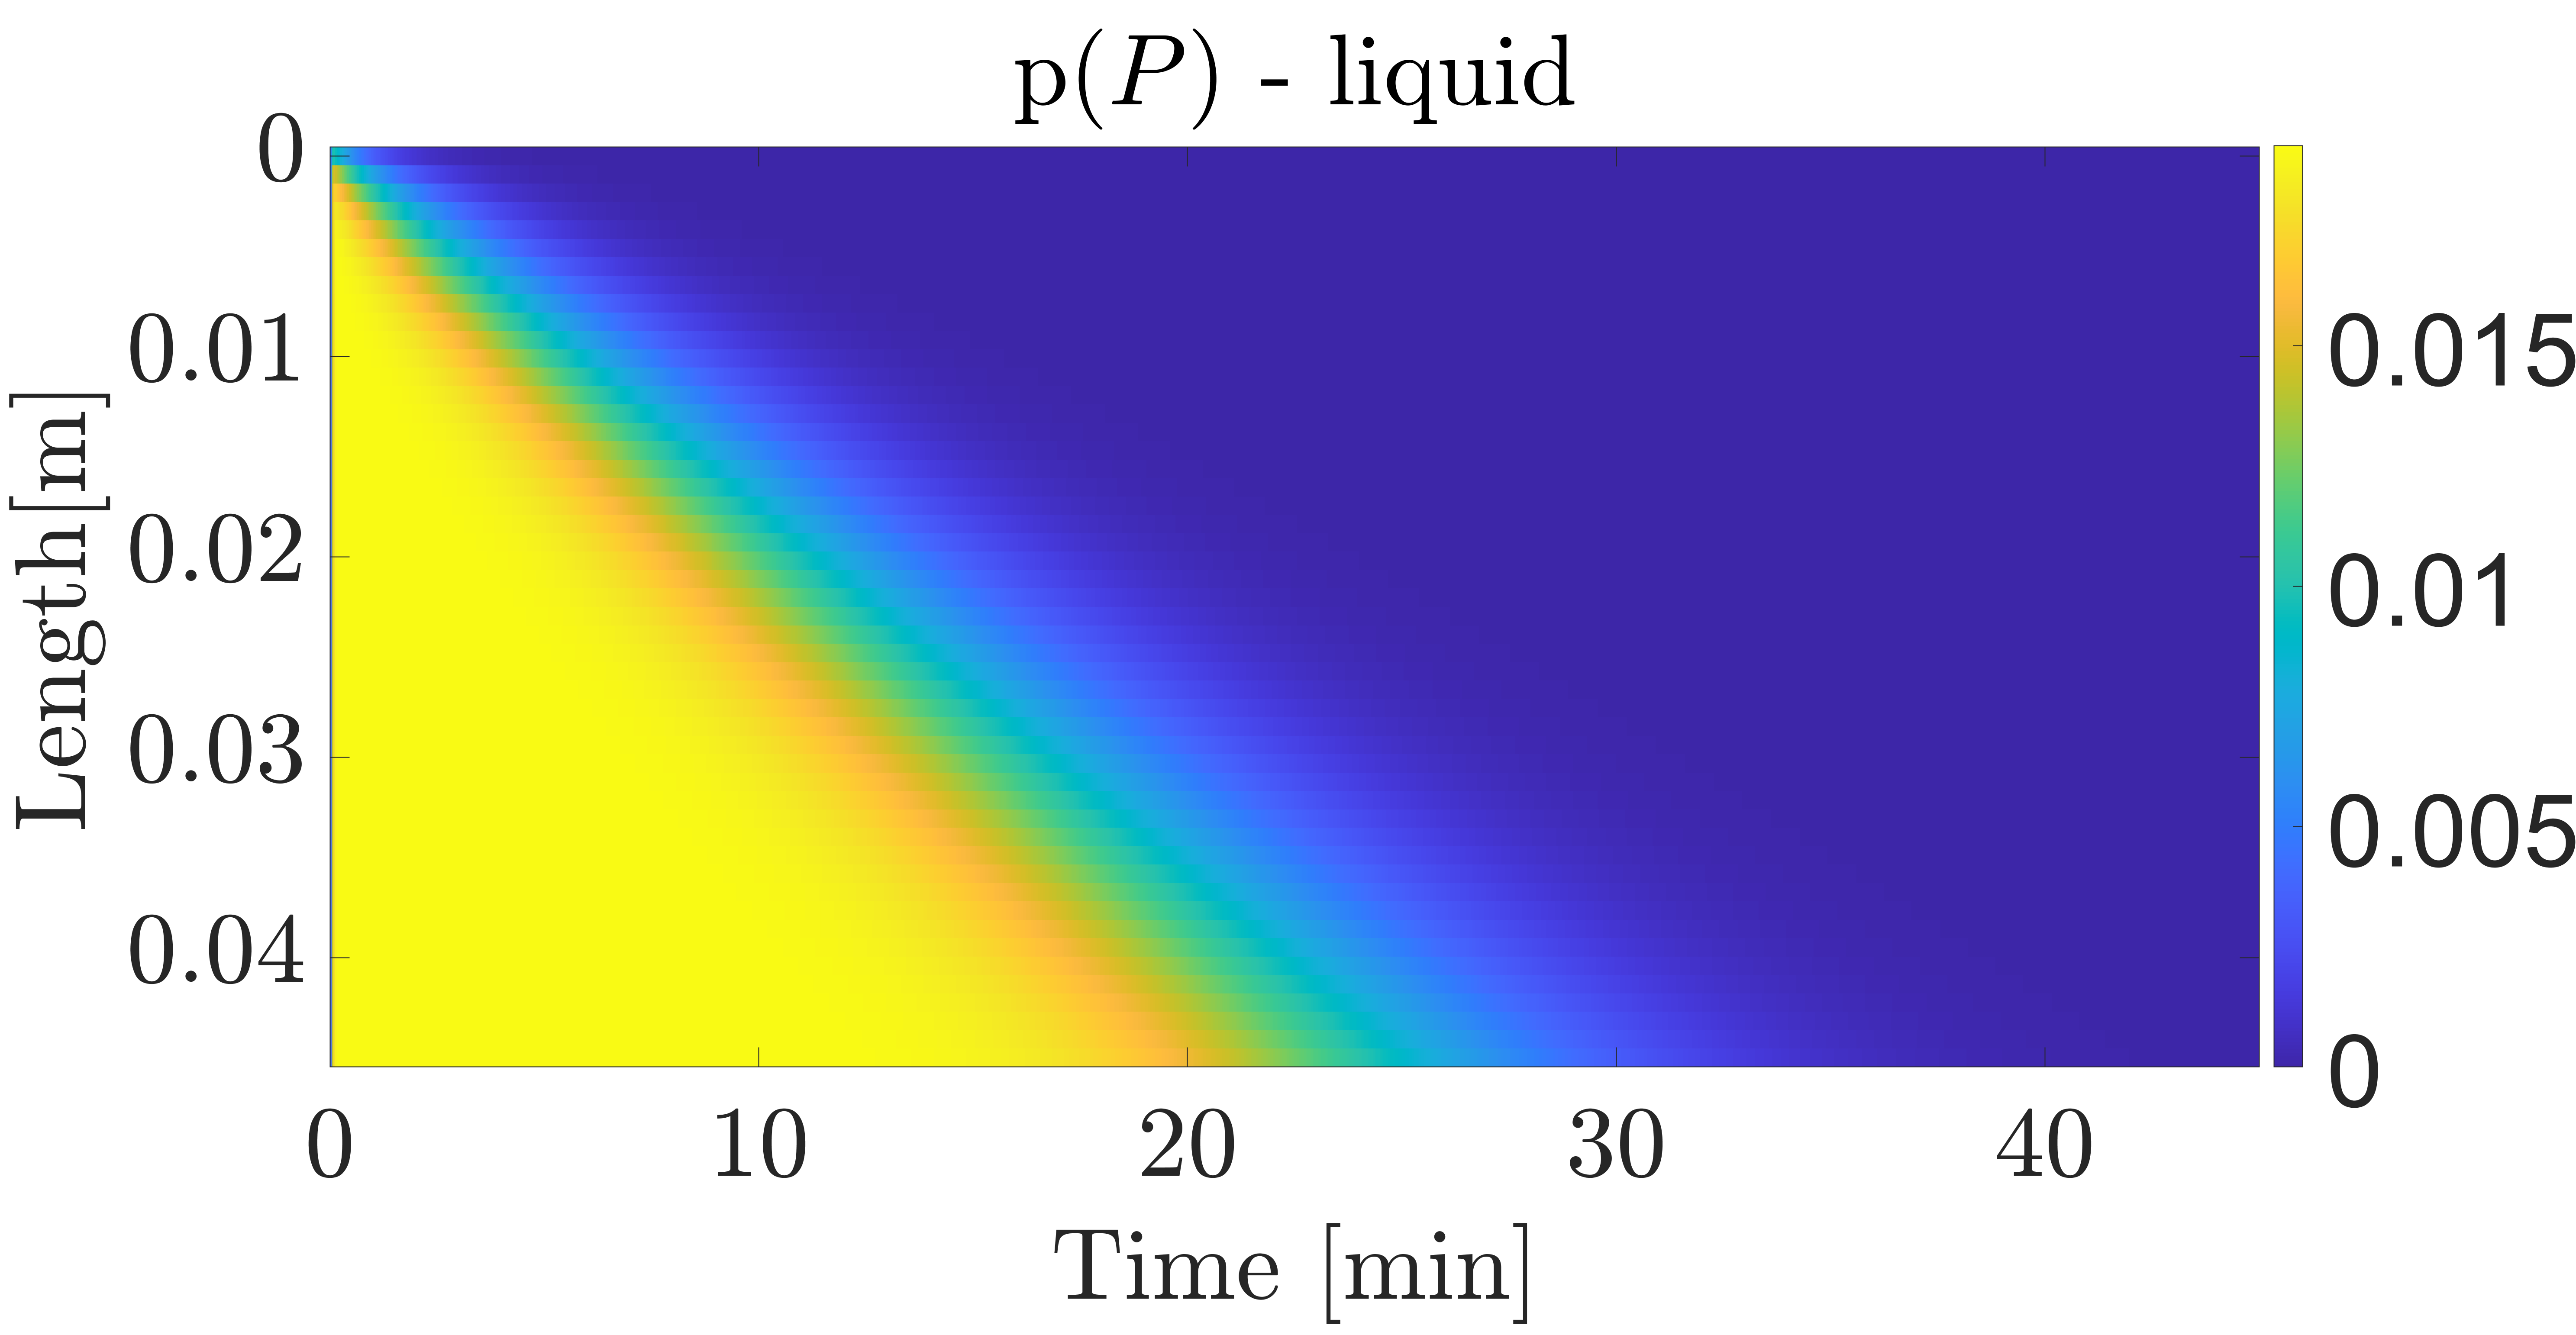
\includegraphics[width=5.5cm,height=2.5cm]{Figures/Sensitivity/Imagesc/2_SS_R_P.png}\\
			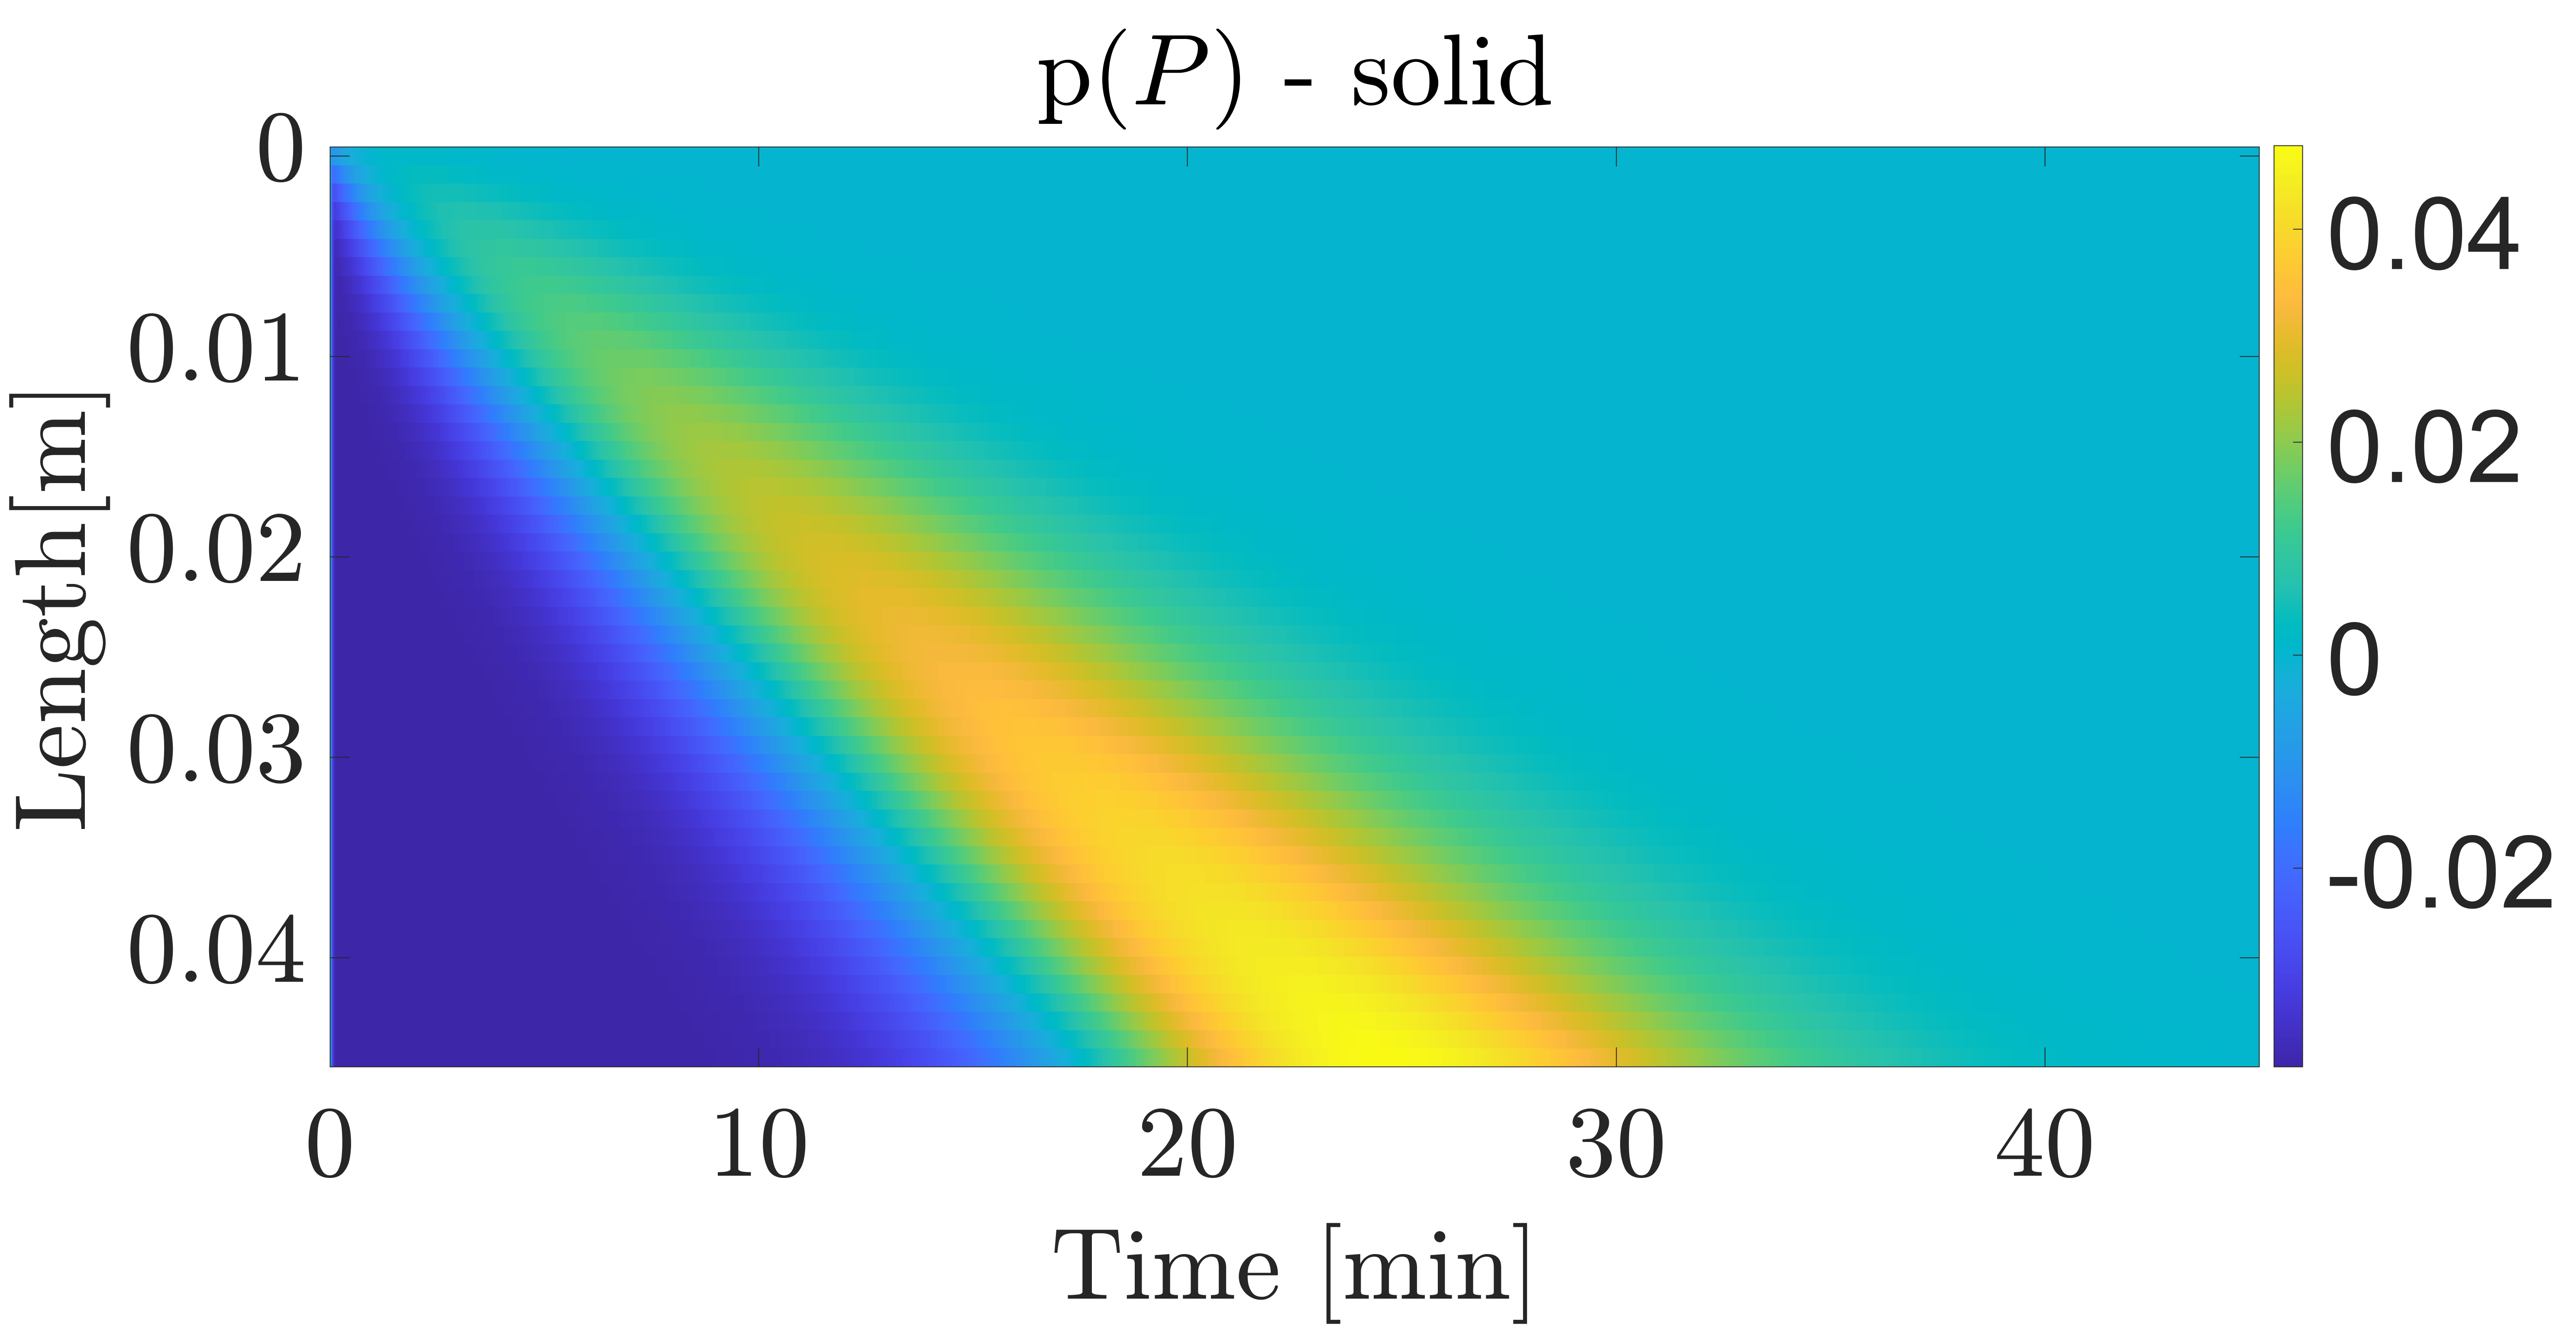
\includegraphics[width=5.5cm,height=2.5cm]{Figures/Sensitivity/Imagesc/3_SS_R_P.png}
		\end{columns}
	\end{frame}

	\begin{frame}[fragile]{Sensitivity Analysis - Pressure}	
		\tiny{
	\begin{align*}
		\cfrac{\partial \textcolor{blue}{c}(t,z)}{\partial t} &=  -\cfrac{F(t)}{\epsilon A\rho(T(t,z)\textcolor{red}{P}(t))} \cfrac{\partial c(t,z)}{\partial z} 
		+ D^M_e(T(t,z)\textcolor{red}{P}(t)) \cfrac{\partial^2 c(t,z)}{\partial z^2} + \cfrac{1-\epsilon}{\epsilon} \cfrac{D_i(T(t,z))}{\mu l^2 }\left(q(t,z) - \cfrac{c(t,z)\rho_s}{k_m(T(t,z))\rho(T(t,z)\textcolor{red}{P}(t))} \right)\\
		\cfrac{\partial \textcolor{blue}{q}(t,z)}{\partial t} &= -\cfrac{D_i(T(t,z))}{\mu l^2 }\left(q(t,z) - c(t,z) \cfrac{\rho_s}{k_m(T(t,z))\rho(T(t,z)\textcolor{red}{P}(t))} \right)\\
		\cfrac{\partial \textcolor{blue}{T}(t,z)}{\partial t} &= -\cfrac{F(t)}{A} \cfrac{C_p(T(t,z)\textcolor{red}{P}(t))}{ [(1-\epsilon)\rho(T(t,z)\textcolor{red}{P}(t)) C_p(T(t,z)\textcolor{red}{P}(t)) + \epsilon \rho_s C_{ps} ]} \cfrac{\partial T(t,z)}{\partial z} 
		+ D^T_e(T(t,z)\textcolor{red}{P}(t)) \cfrac{\partial^2 T(t,z)}{\partial z^2}\\
	\end{align*}}		
		\begin{columns}[t]
			\column{.5\textwidth}
			\centering
			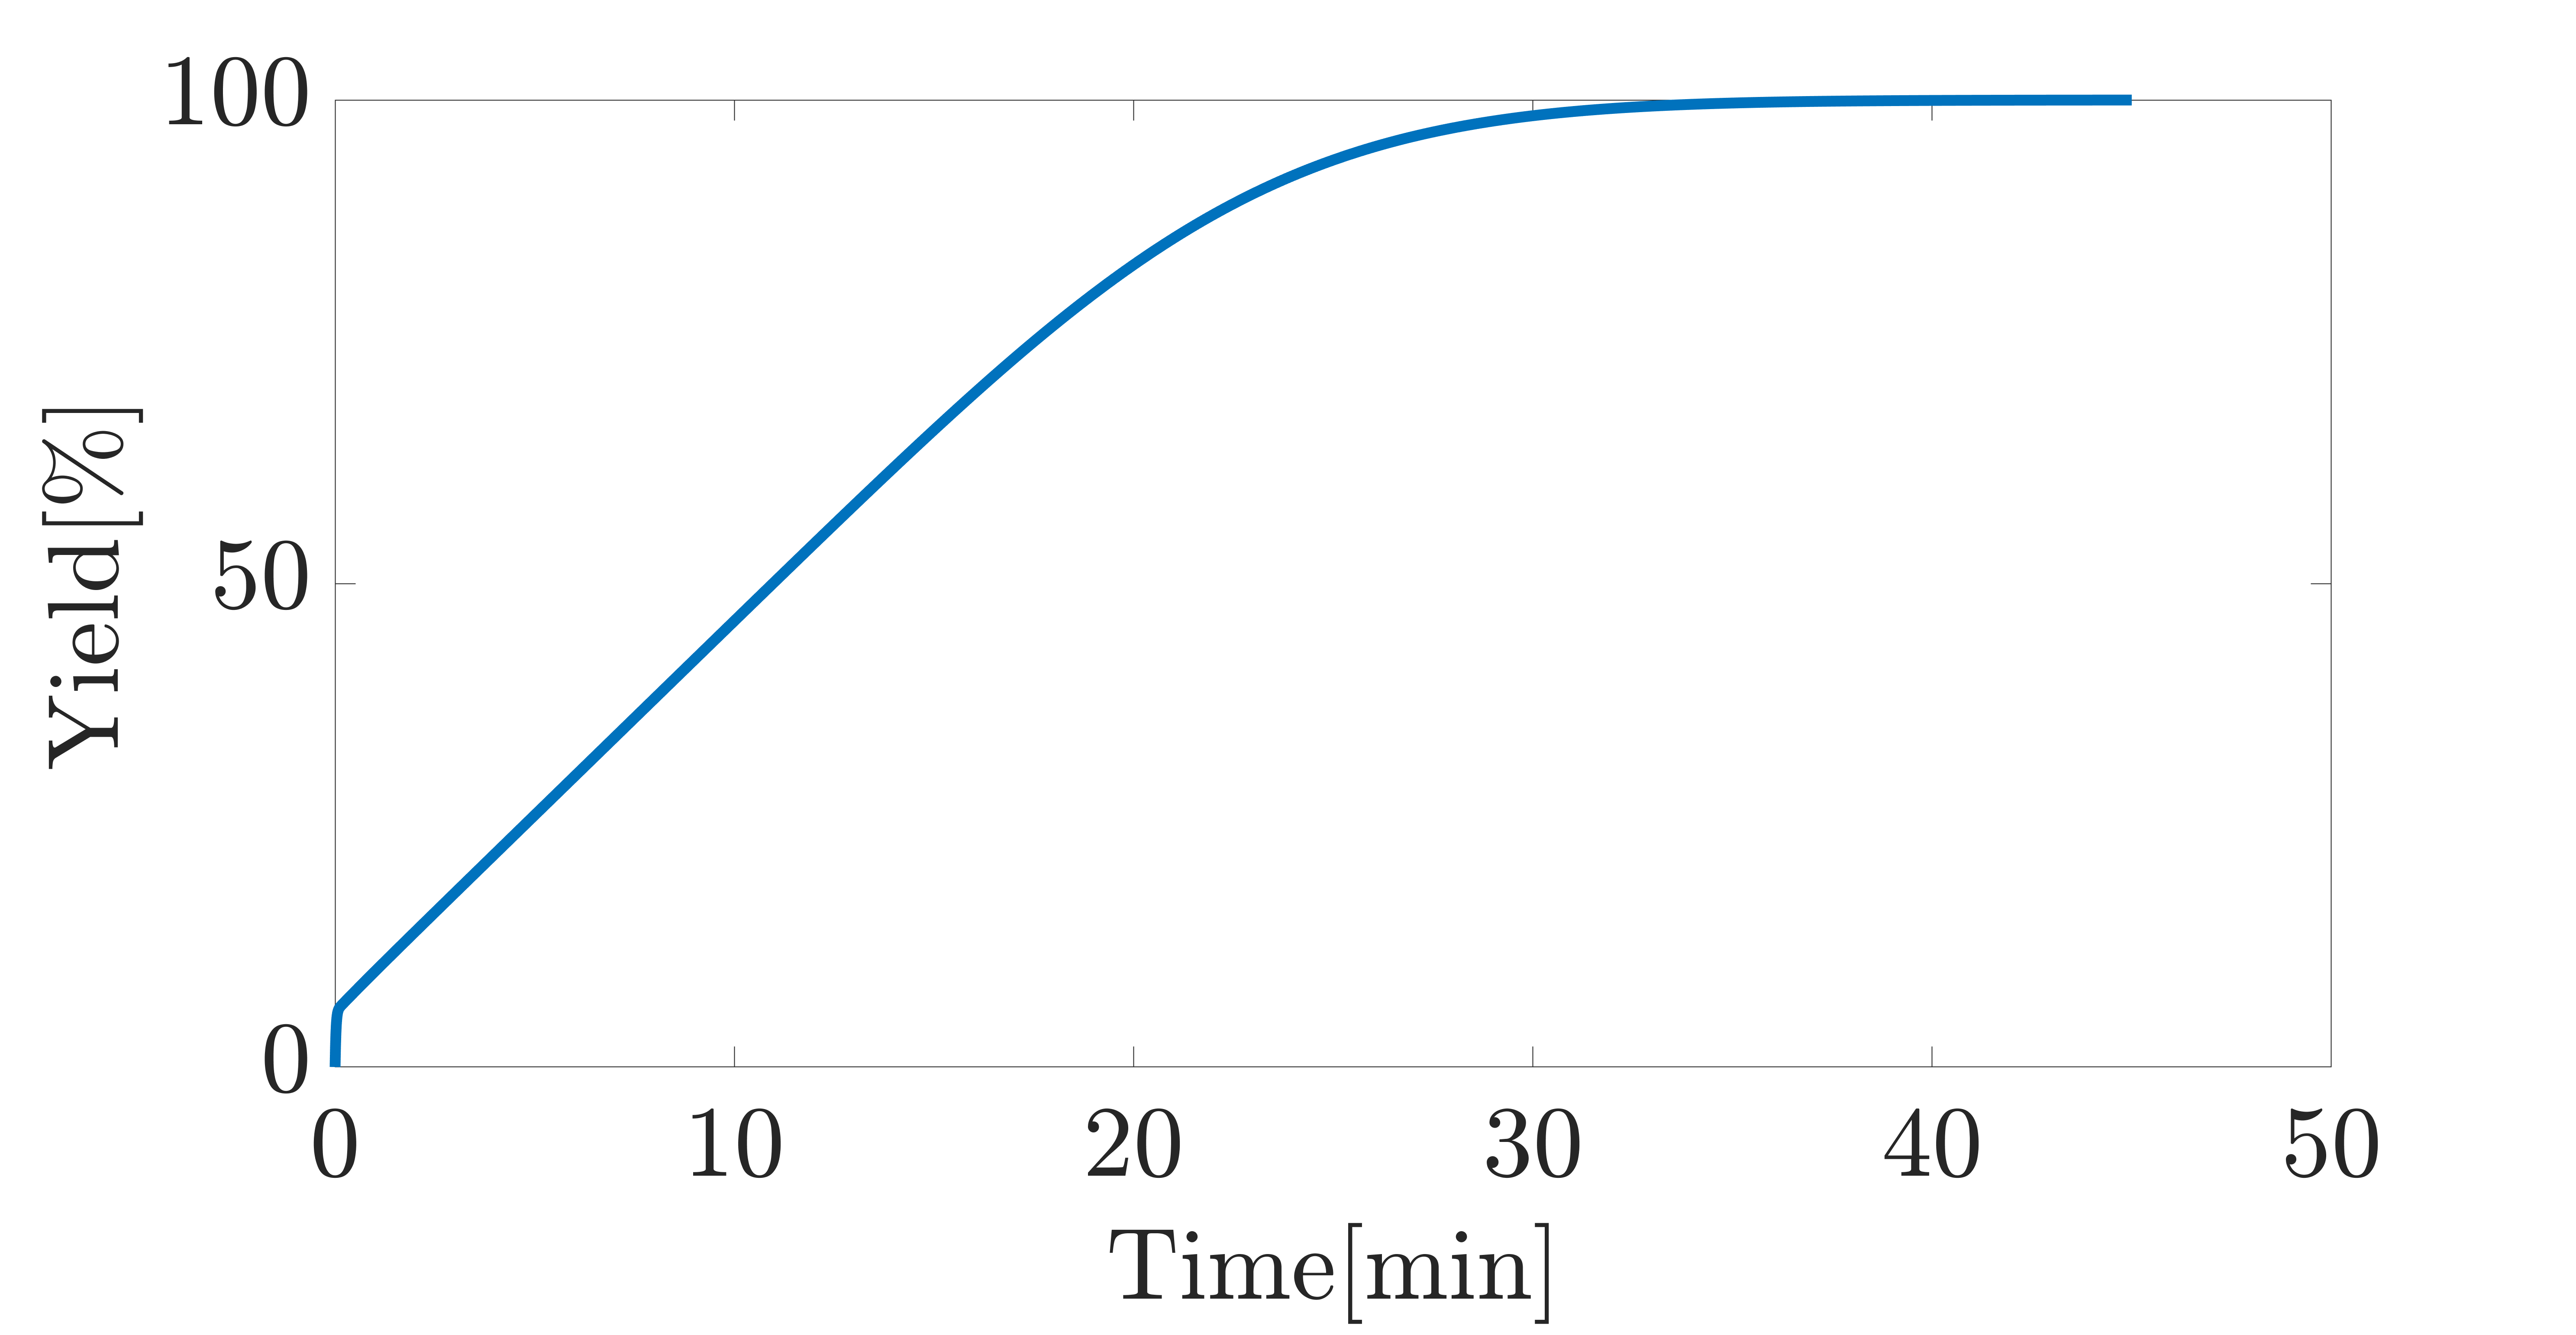
\includegraphics[width=5.5cm,height=2.5cm]{Figures/Sensitivity/Yield.png}\\
			\column{.5\textwidth}
			\centering
			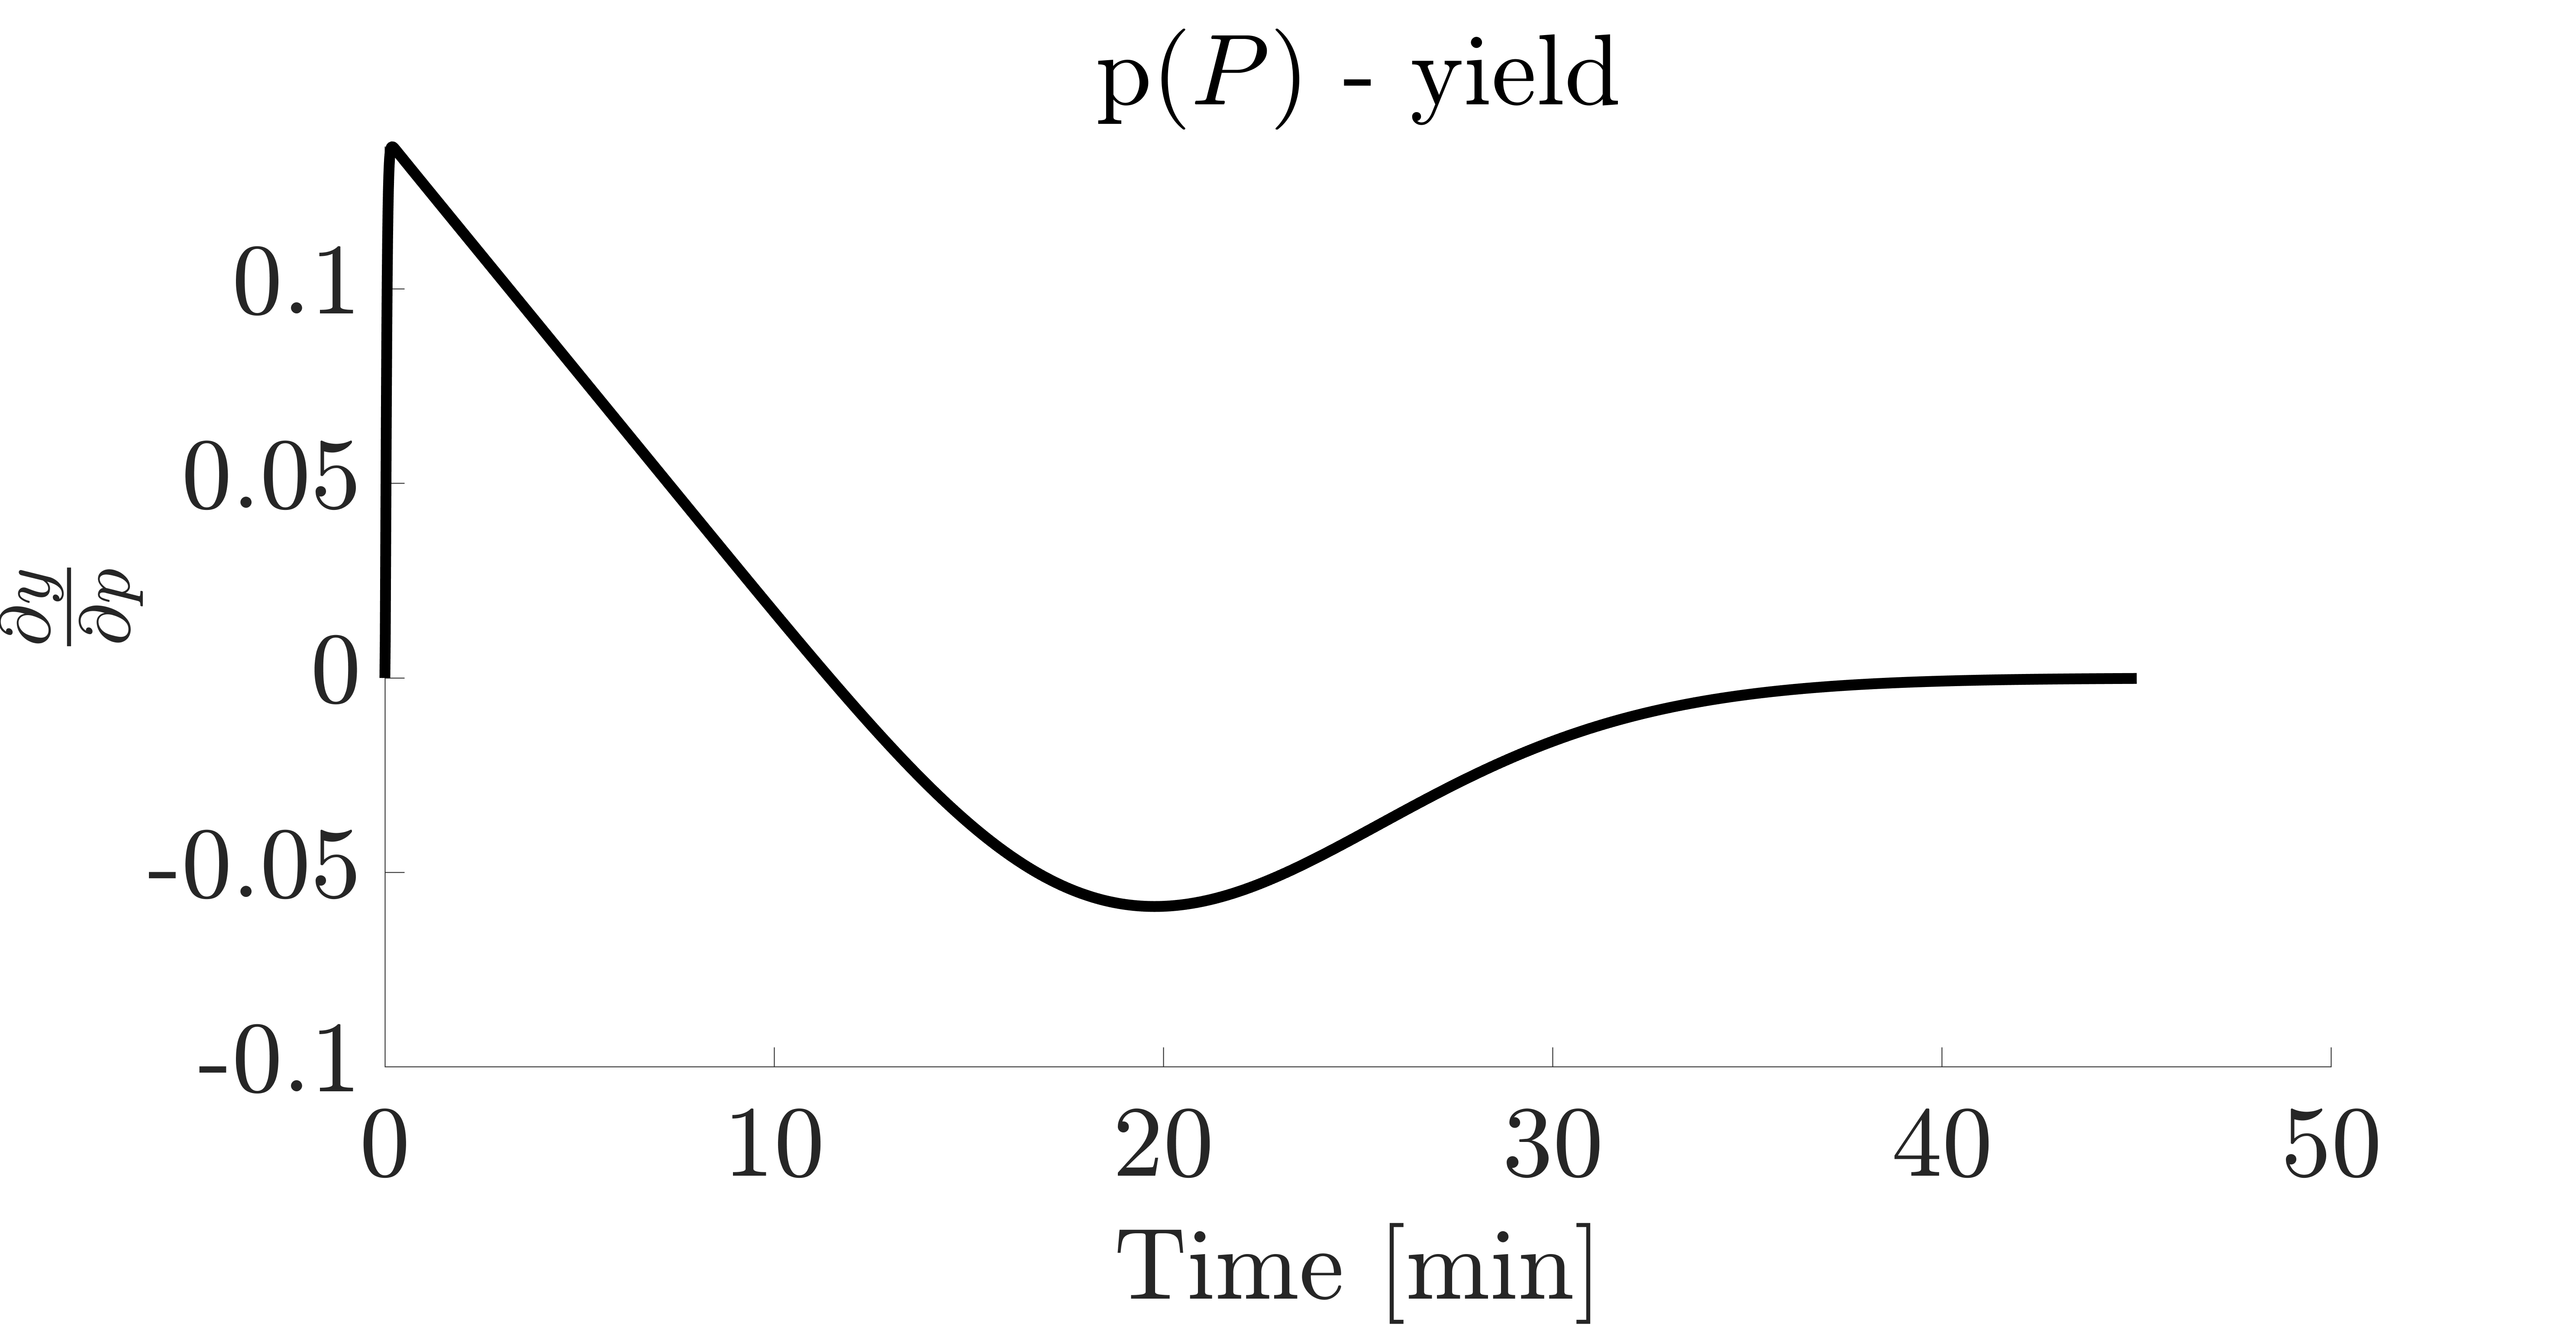
\includegraphics[width=5.5cm,height=2.5cm]{Figures/Sensitivity/Plots/1_SS_R_P.png}\\
		\end{columns}	
	\end{frame}

	\begin{frame}[fragile]{Sensitivity Analysis - Void Fraction}
		\tiny{
			\begin{align*}
				\cfrac{\partial \textcolor{blue}{c}(t,z)}{\partial t} &=  -\cfrac{F(t)}{\textcolor{green}{\epsilon}A\rho(T(t,z)P(t))} \cfrac{\partial c(t,z)}{\partial z}
				+ D^M_e(T(t,z)P(t)) \cfrac{\partial^2 c(t,z)}{\partial z^2} + \cfrac{1-\textcolor{green}{\epsilon}}{\textcolor{green}{\epsilon}} \cfrac{D_i(T(t,z))}{\mu l^2 }\left(q(t,z) - \cfrac{c(t,z)\rho_s}{k_m(T(t,z))\rho(T(t,z)P(t))} \right)\\
				\cfrac{\partial \textcolor{blue}{q}(t,z)}{\partial t} &= -\cfrac{D_i(T(t,z))}{\mu l^2}\left(q(t,z) - c(t,z) \cfrac{\rho_s}{k_m(T(t,z))\rho(T(t,z)P(t))} \right)\\
				\cfrac{\partial \textcolor{blue}{T}(t,z)}{\partial t} &= -\cfrac{F(t)}{A} \cfrac{C_p(T(t,z)P(t))}{ [(1-\textcolor{green}{\epsilon})\rho(T(t,z)P(t)) C_p(T(t,z)P(t)) + \textcolor{green}{ \epsilon}\rho_s C_{ps} ]} \cfrac{\partial T(t,z)}{\partial z} 
				+  D^T_e(T(t,z)P(t)) \cfrac{\partial^2 T(t,z)}{\partial z^2}
		\end{align*}}
		\begin{columns}[t]
			\column{.5\textwidth}
			\centering
			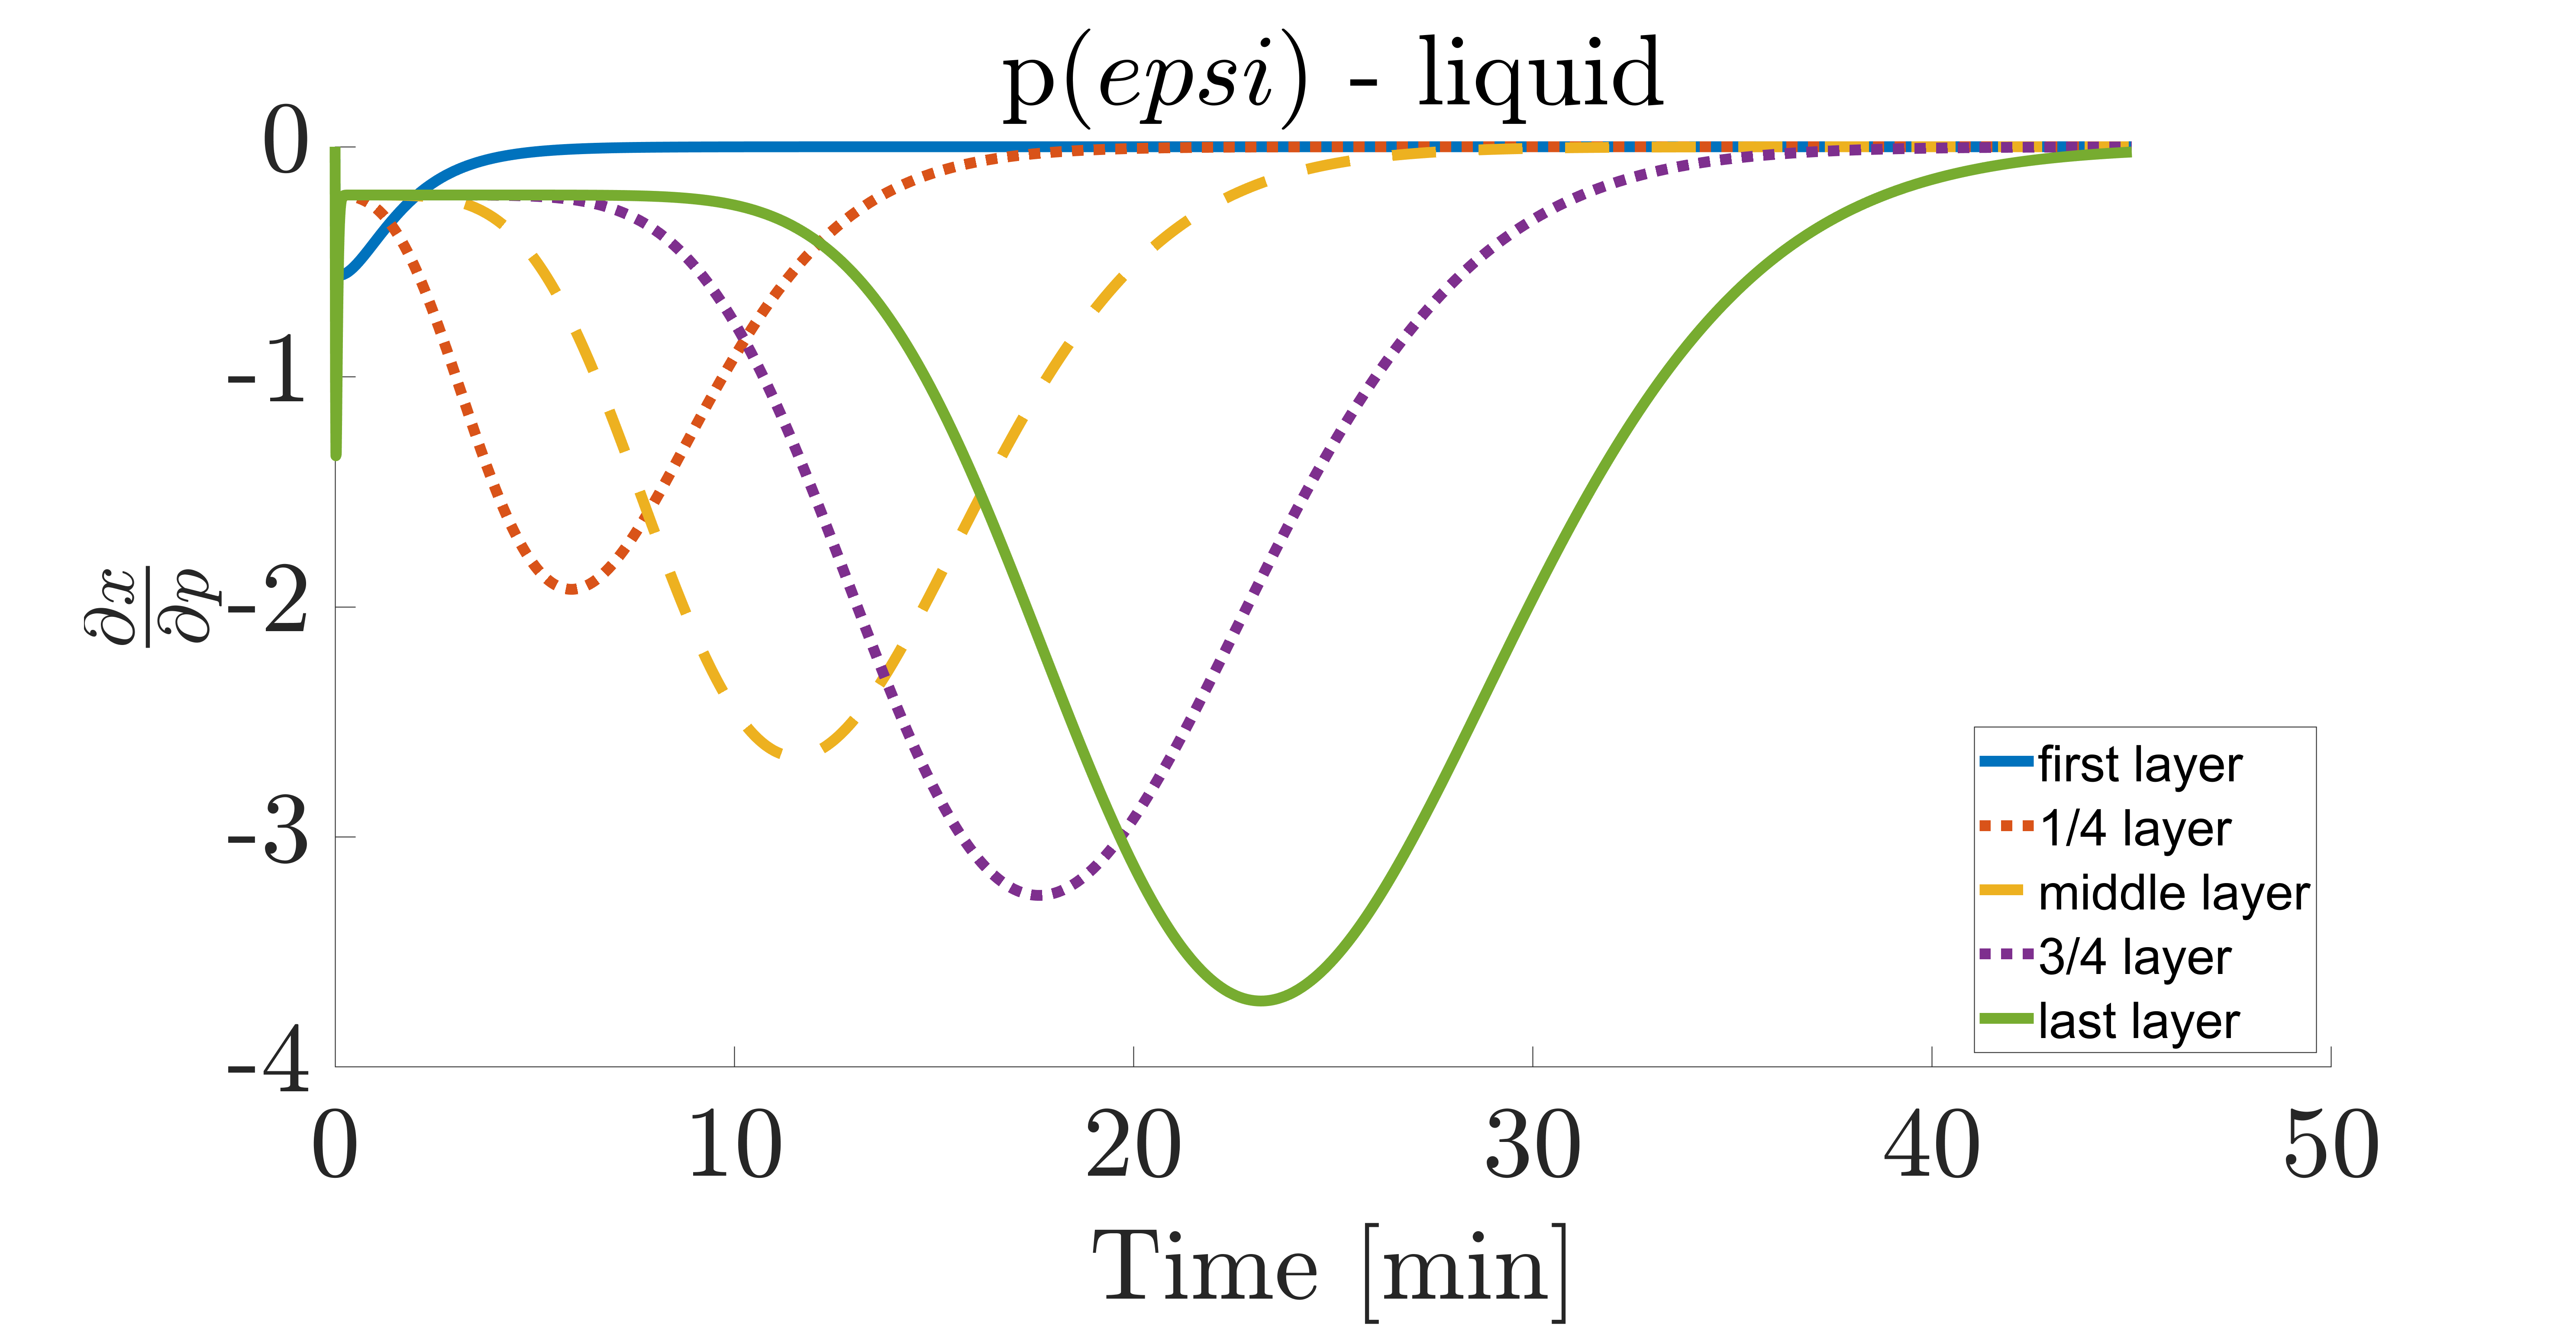
\includegraphics[width=5.5cm,height=2.5cm]{Figures/Sensitivity/Plots/2_SS_R_epsi.png}\\
			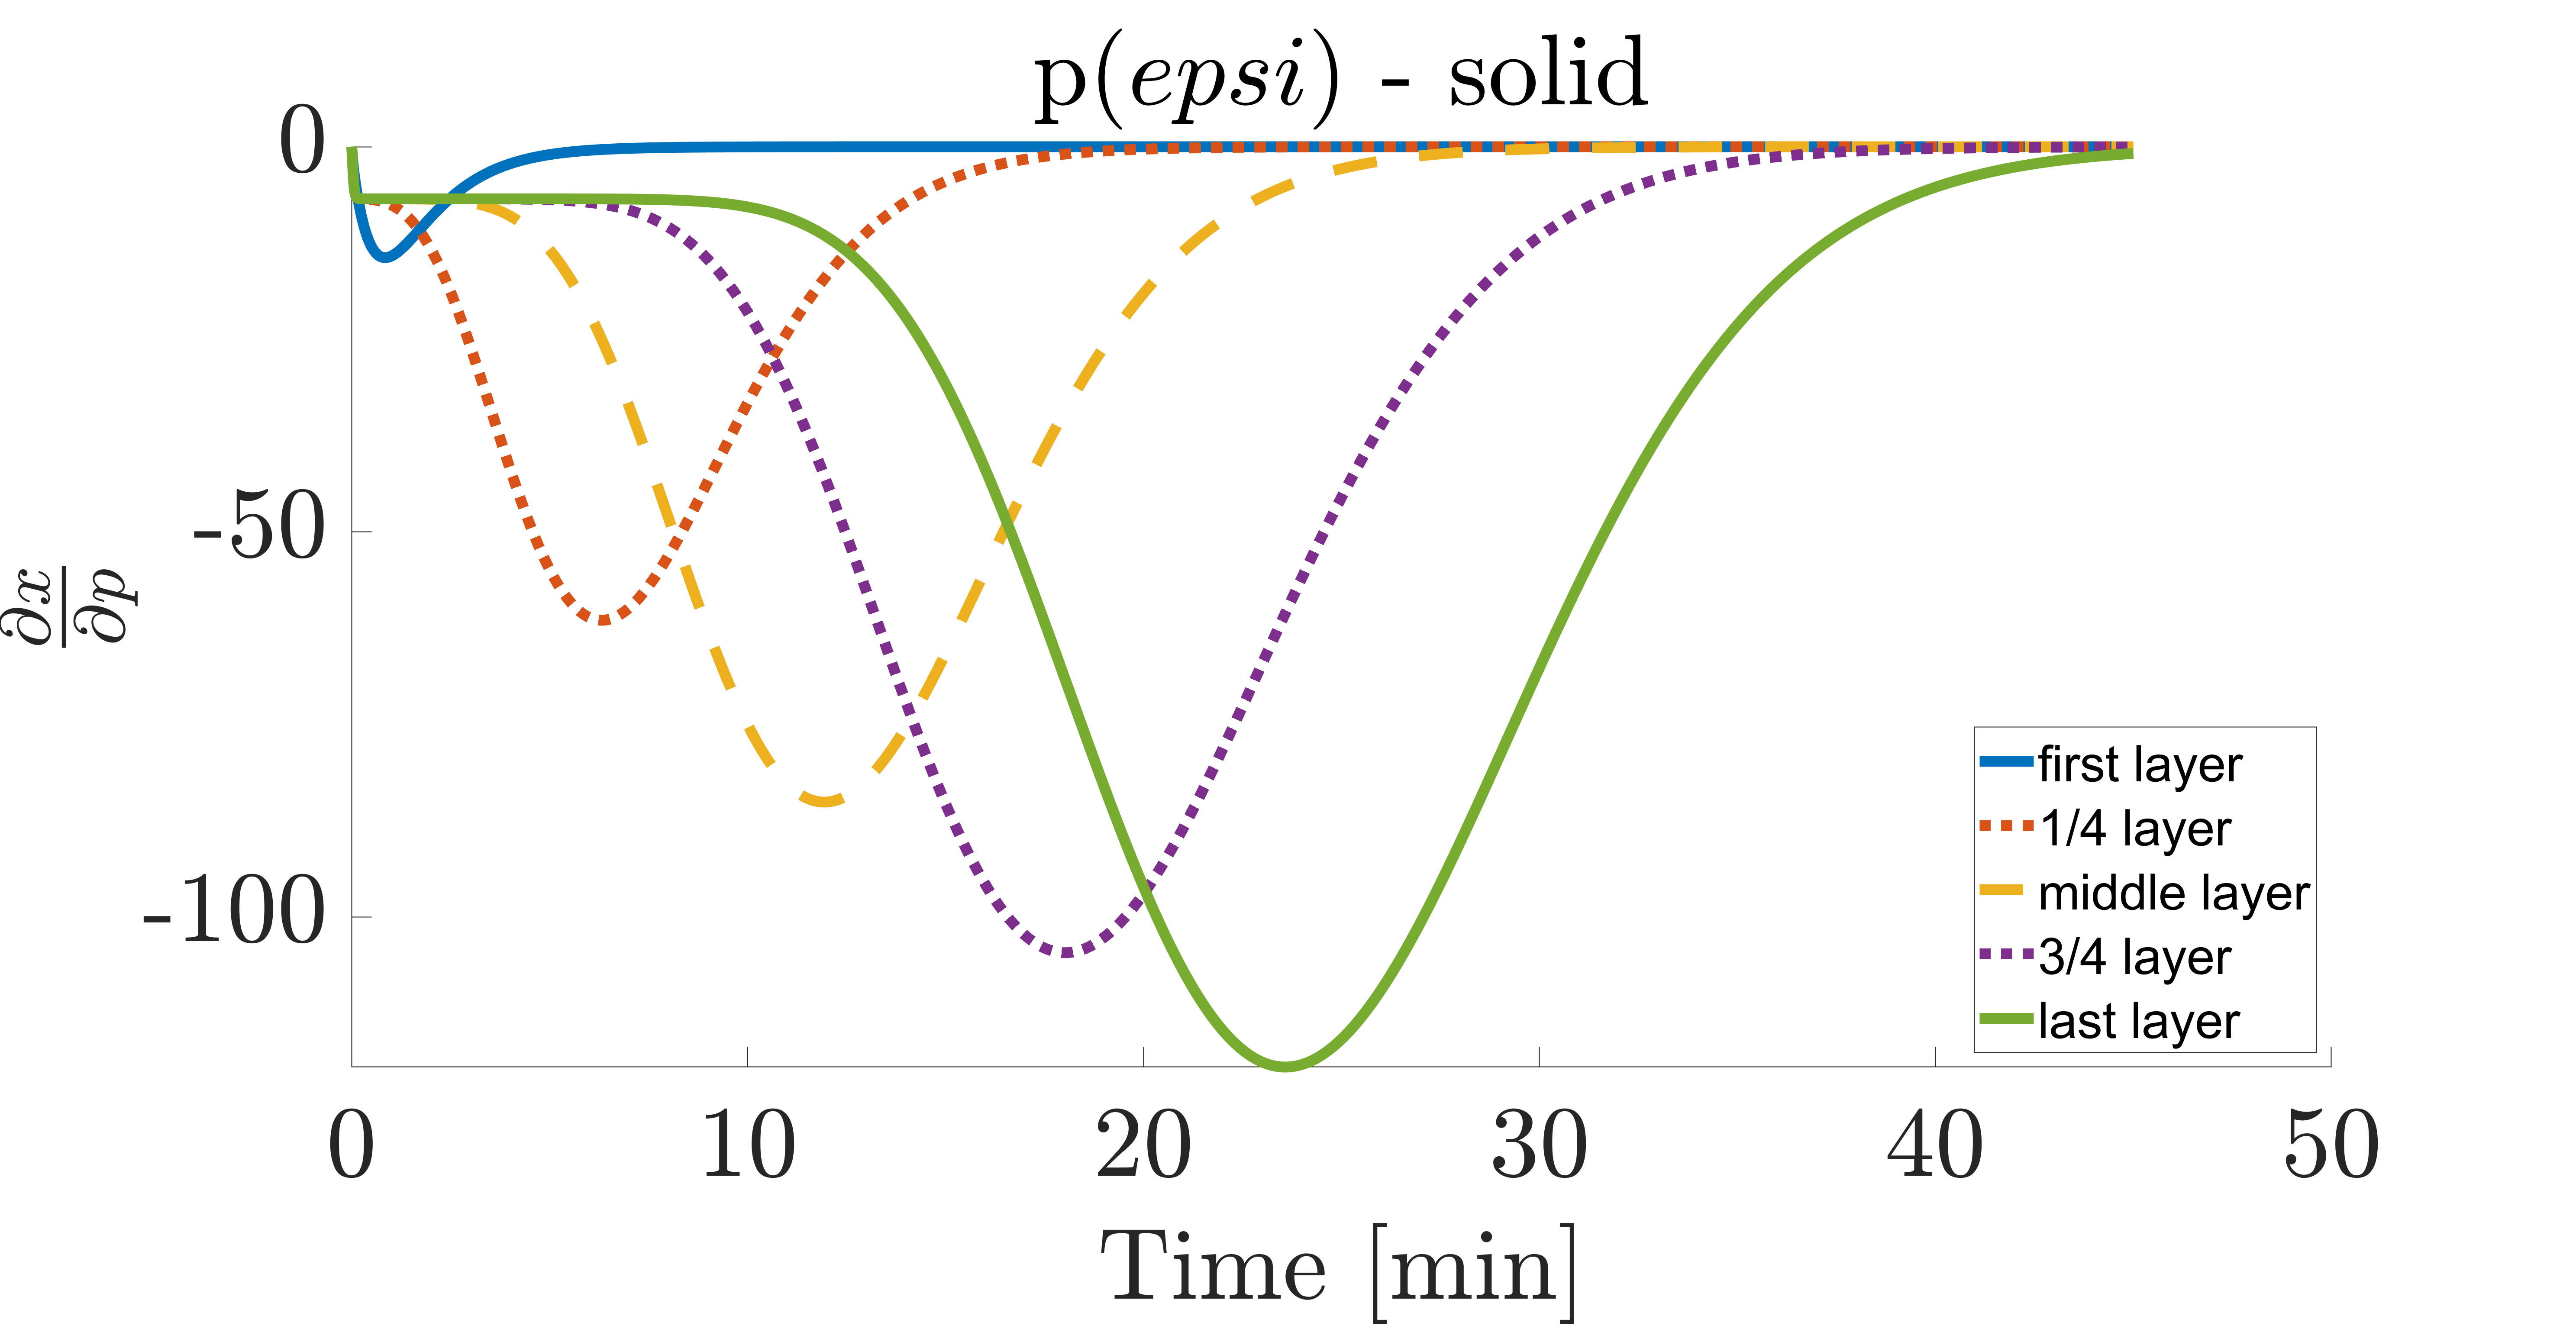
\includegraphics[width=5.5cm,height=2.5cm]{Figures/Sensitivity/Plots/3_SS_R_epsi.png}
			\column{.5\textwidth}
			\centering
			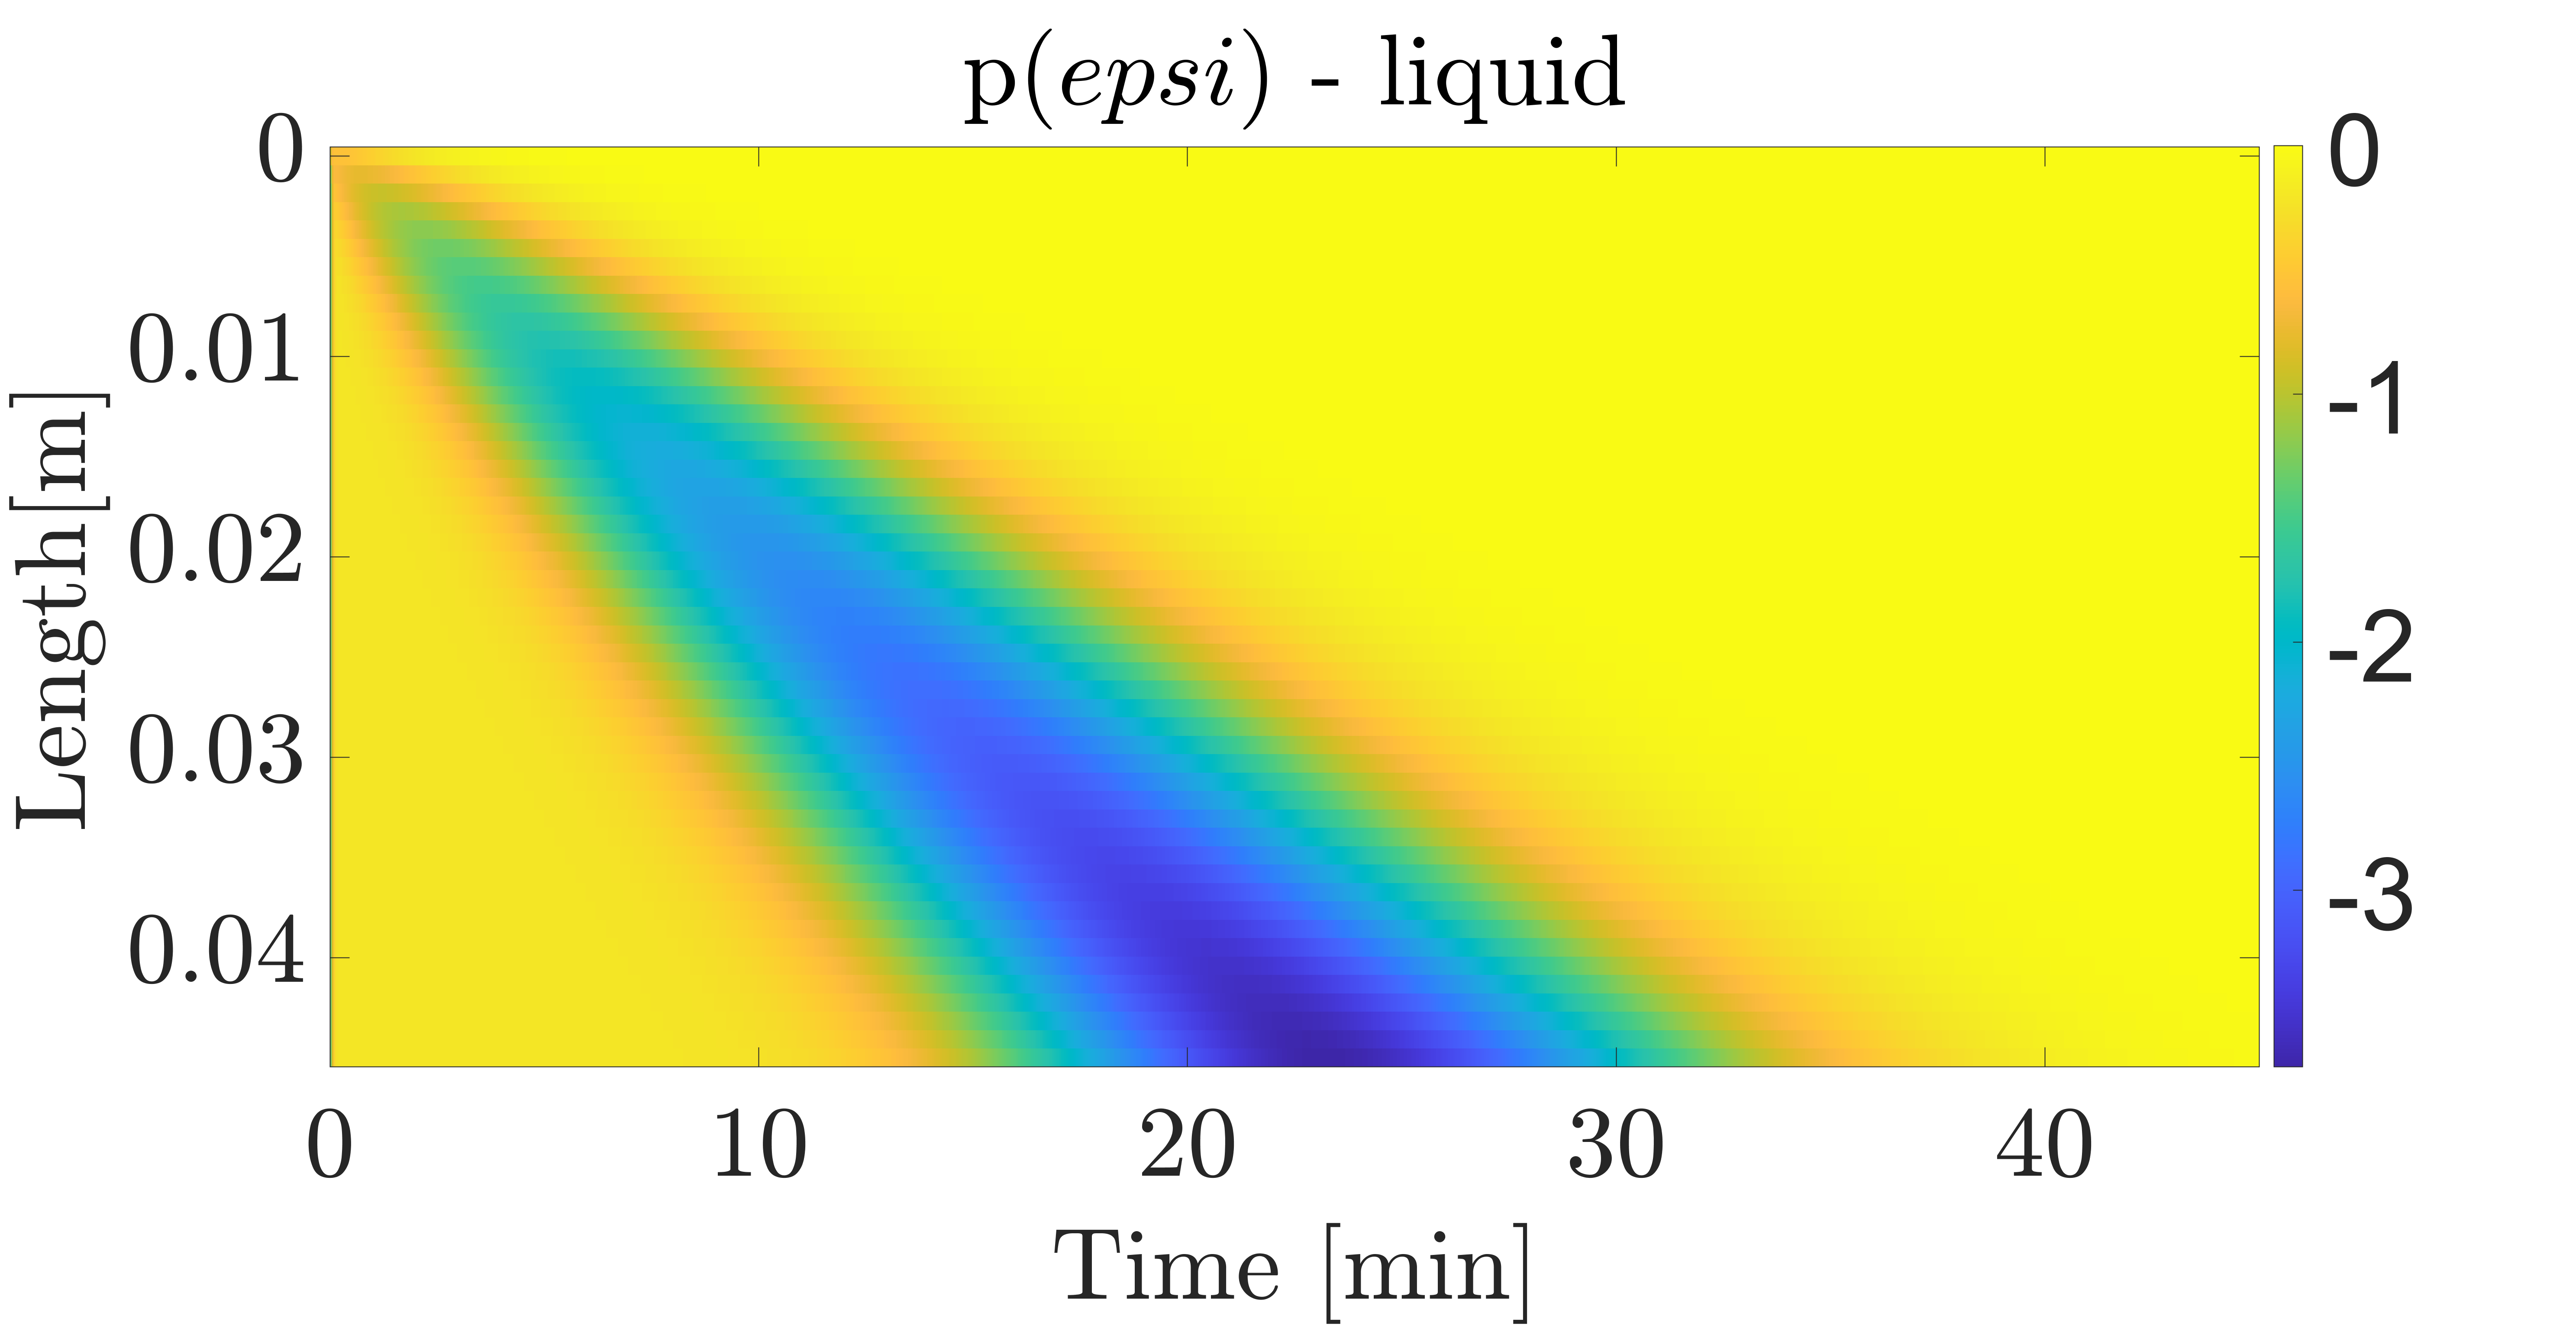
\includegraphics[width=5.5cm,height=2.5cm]{Figures/Sensitivity/Imagesc/2_SS_R_epsi.png}\\
			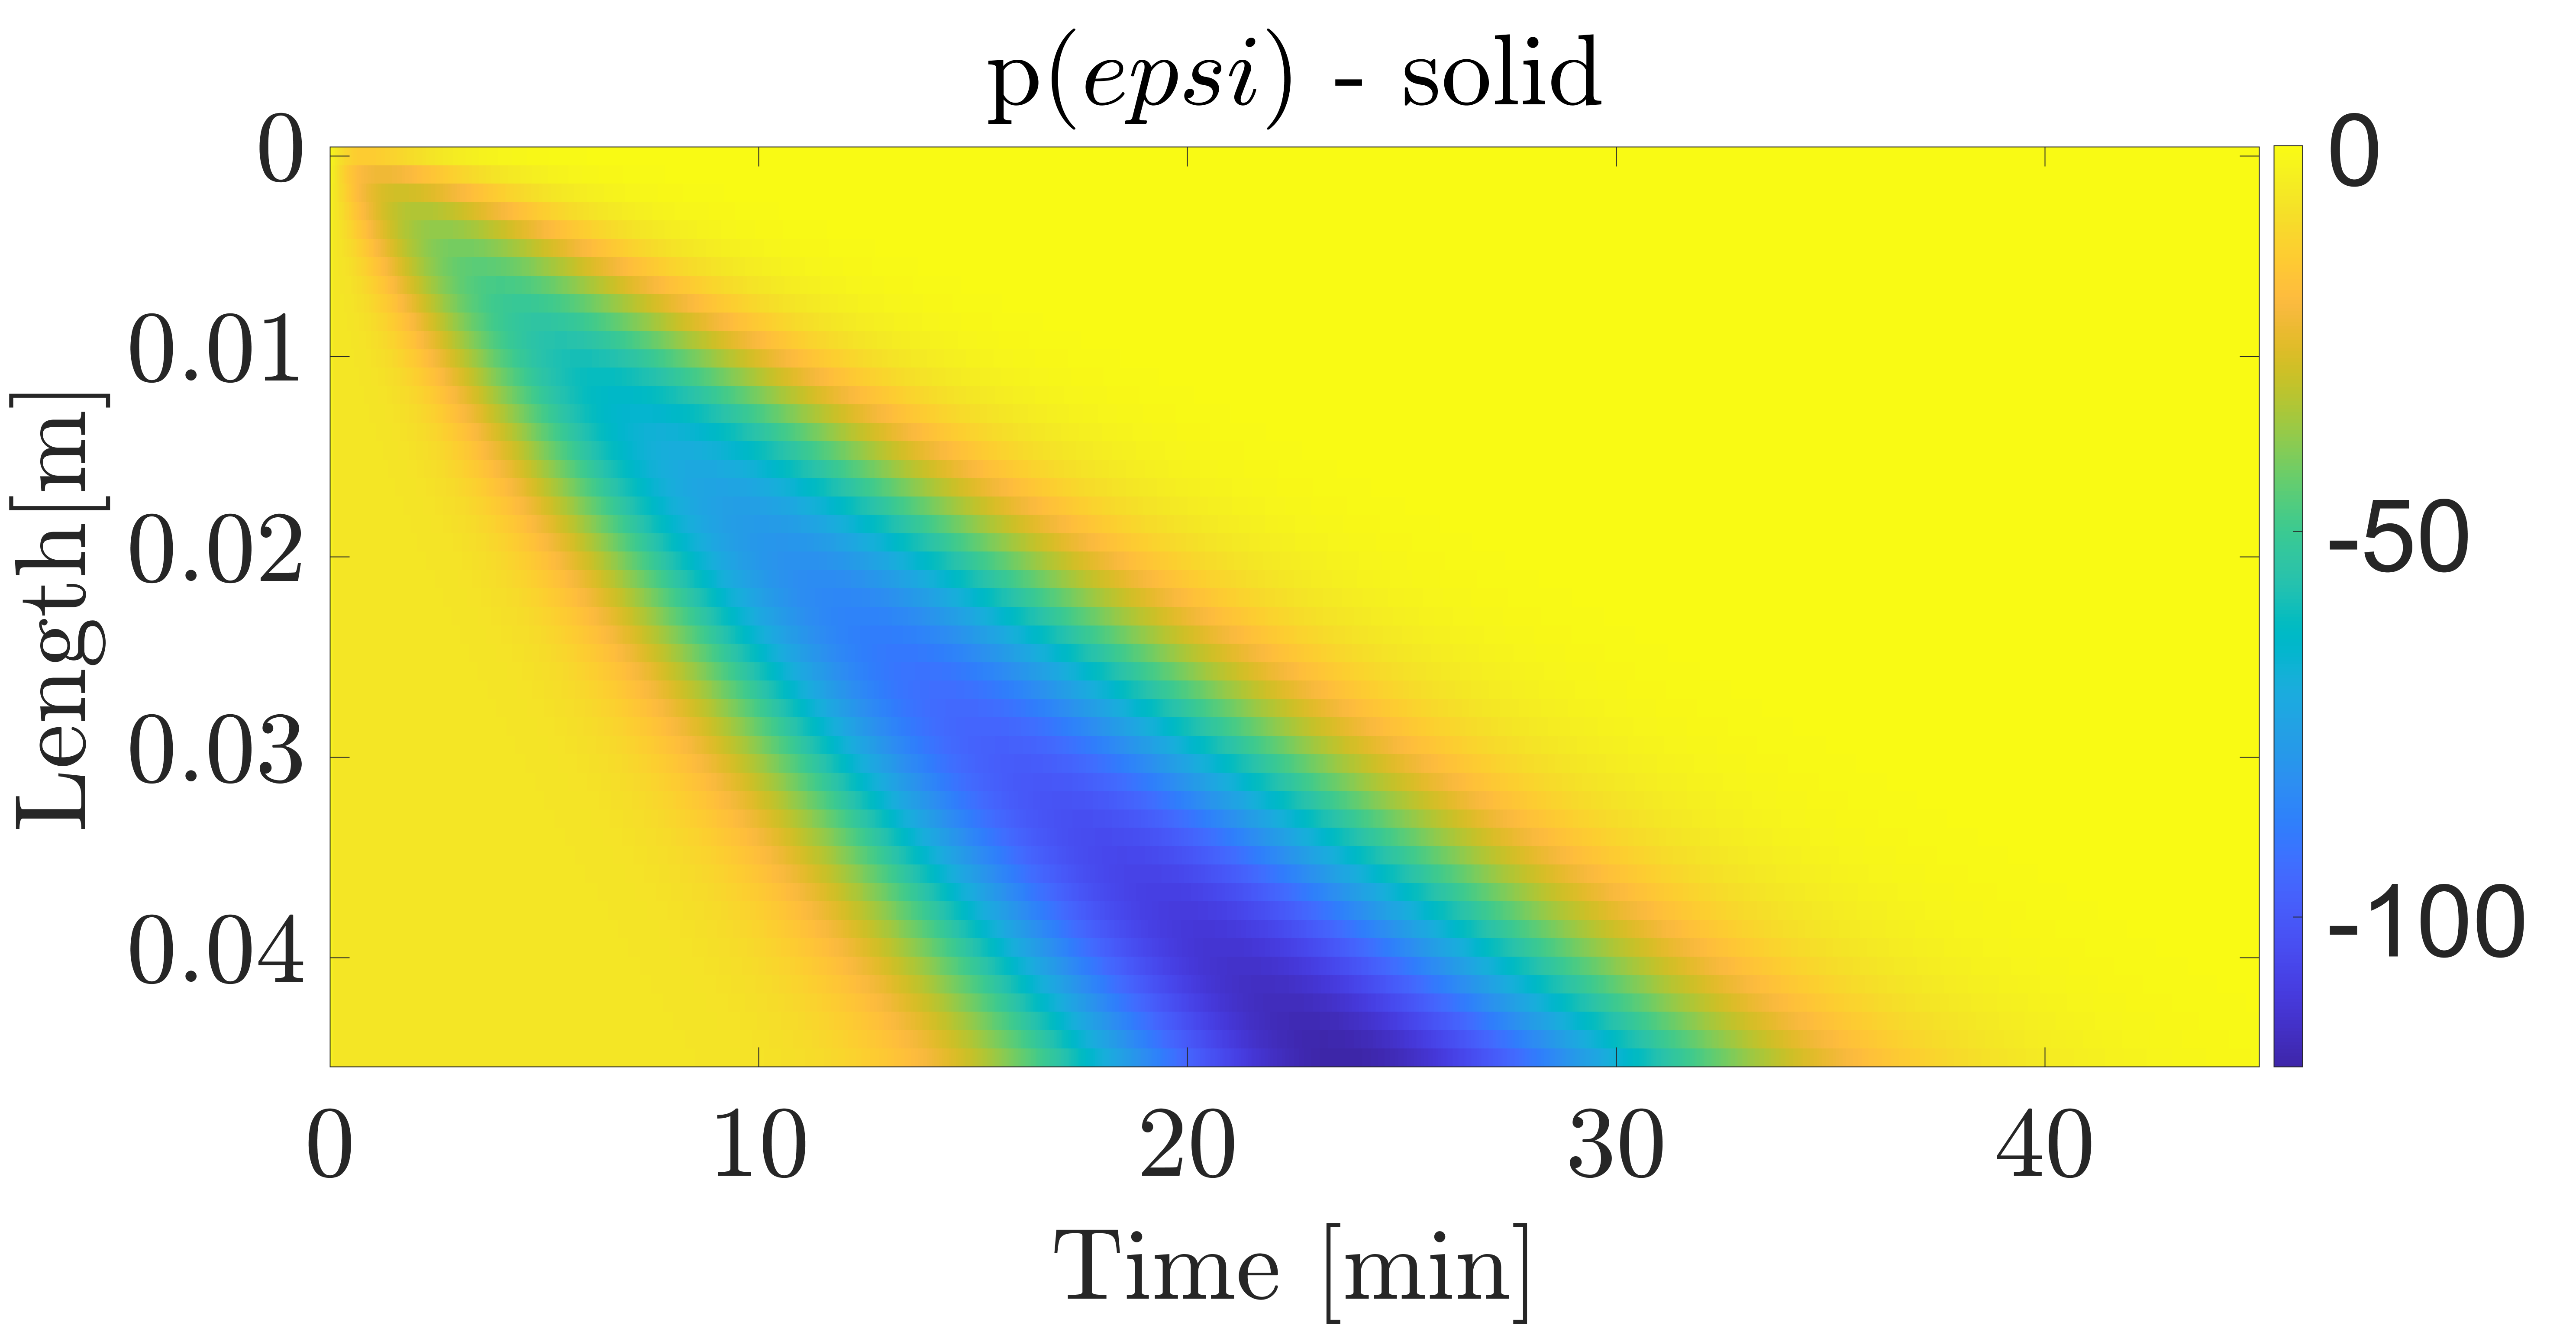
\includegraphics[width=5.5cm,height=2.5cm]{Figures/Sensitivity/Imagesc/3_SS_R_epsi.png}
		\end{columns}
	\end{frame}
	
	\begin{frame}[fragile]{Sensitivity Analysis - Void Fraction}	
		\tiny{
			\begin{align*}
				\cfrac{\partial \textcolor{blue}{c}(t,z)}{\partial t} &=  -\cfrac{F(t)}{\textcolor{green}{\epsilon}A\rho(T(t,z)P(t))} \cfrac{\partial c(t,z)}{\partial z}
				+ D^M_e(T(t,z)P(t)) \cfrac{\partial^2 c(t,z)}{\partial z^2} + \cfrac{1-\textcolor{green}{\epsilon}}{\textcolor{green}{\epsilon}} 	\cfrac{D_i(T(t,z))}{\mu l^2 }\left(q(t,z) - \cfrac{c(t,z)\rho_s}{k_m(T(t,z))\rho(T(t,z)P(t))} \right)\\
				\cfrac{\partial \textcolor{blue}{q}(t,z)}{\partial t} &= -\cfrac{D_i(T(t,z))}{\mu l^2}\left(q(t,z) - c(t,z) 	\cfrac{\rho_s}{k_m(T(t,z))\rho(T(t,z)P(t))} \right)\\
				\cfrac{\partial \textcolor{blue}{T}(t,z)}{\partial t} &= -\cfrac{F(t)}{A} \cfrac{C_p(T(t,z)P(t))}{ 	[(1-\textcolor{green}{\epsilon})\rho(T(t,z)P(t)) C_p(T(t,z)P(t)) + \textcolor{green}{ \epsilon}\rho_s C_{ps} ]} \cfrac{\partial T(t,z)}{\partial z} 
				+  D^T_e(T(t,z)P(t)) \cfrac{\partial^2 T(t,z)}{\partial z^2}\\
		\end{align*}}		
		\begin{columns}[t]
			\column{.5\textwidth}
			\centering
			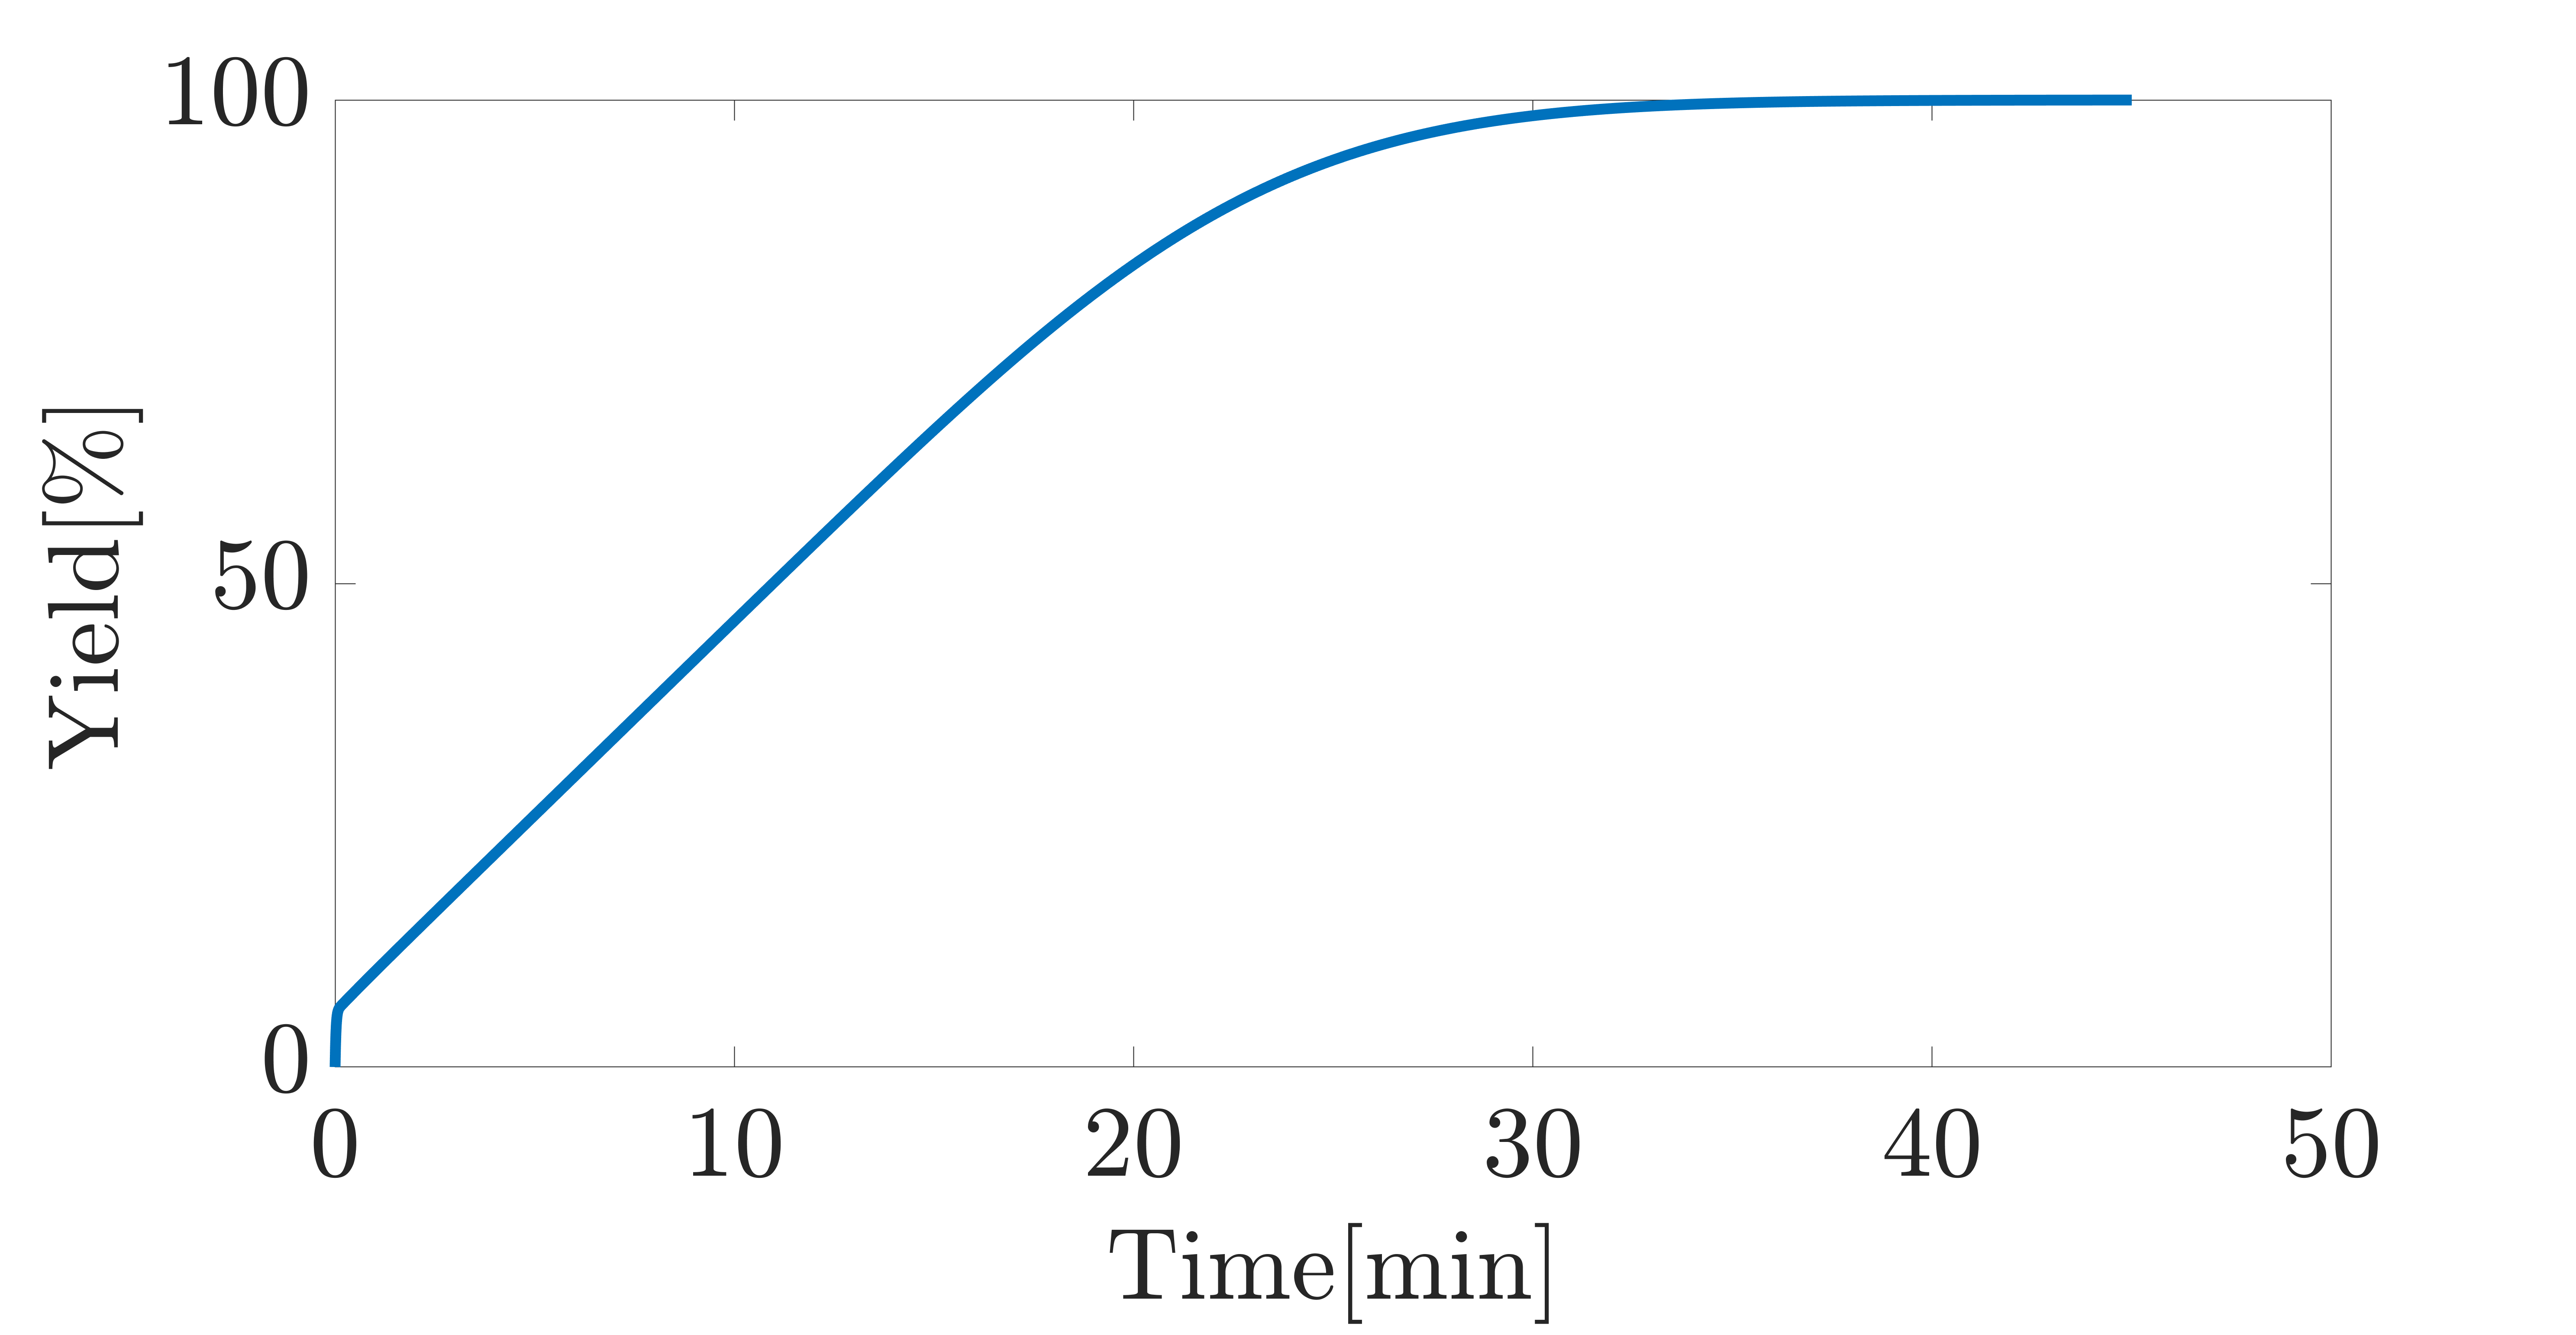
\includegraphics[width=5.5cm,height=2.5cm]{Figures/Sensitivity/Yield.png}\\
			\column{.5\textwidth}
			\centering
			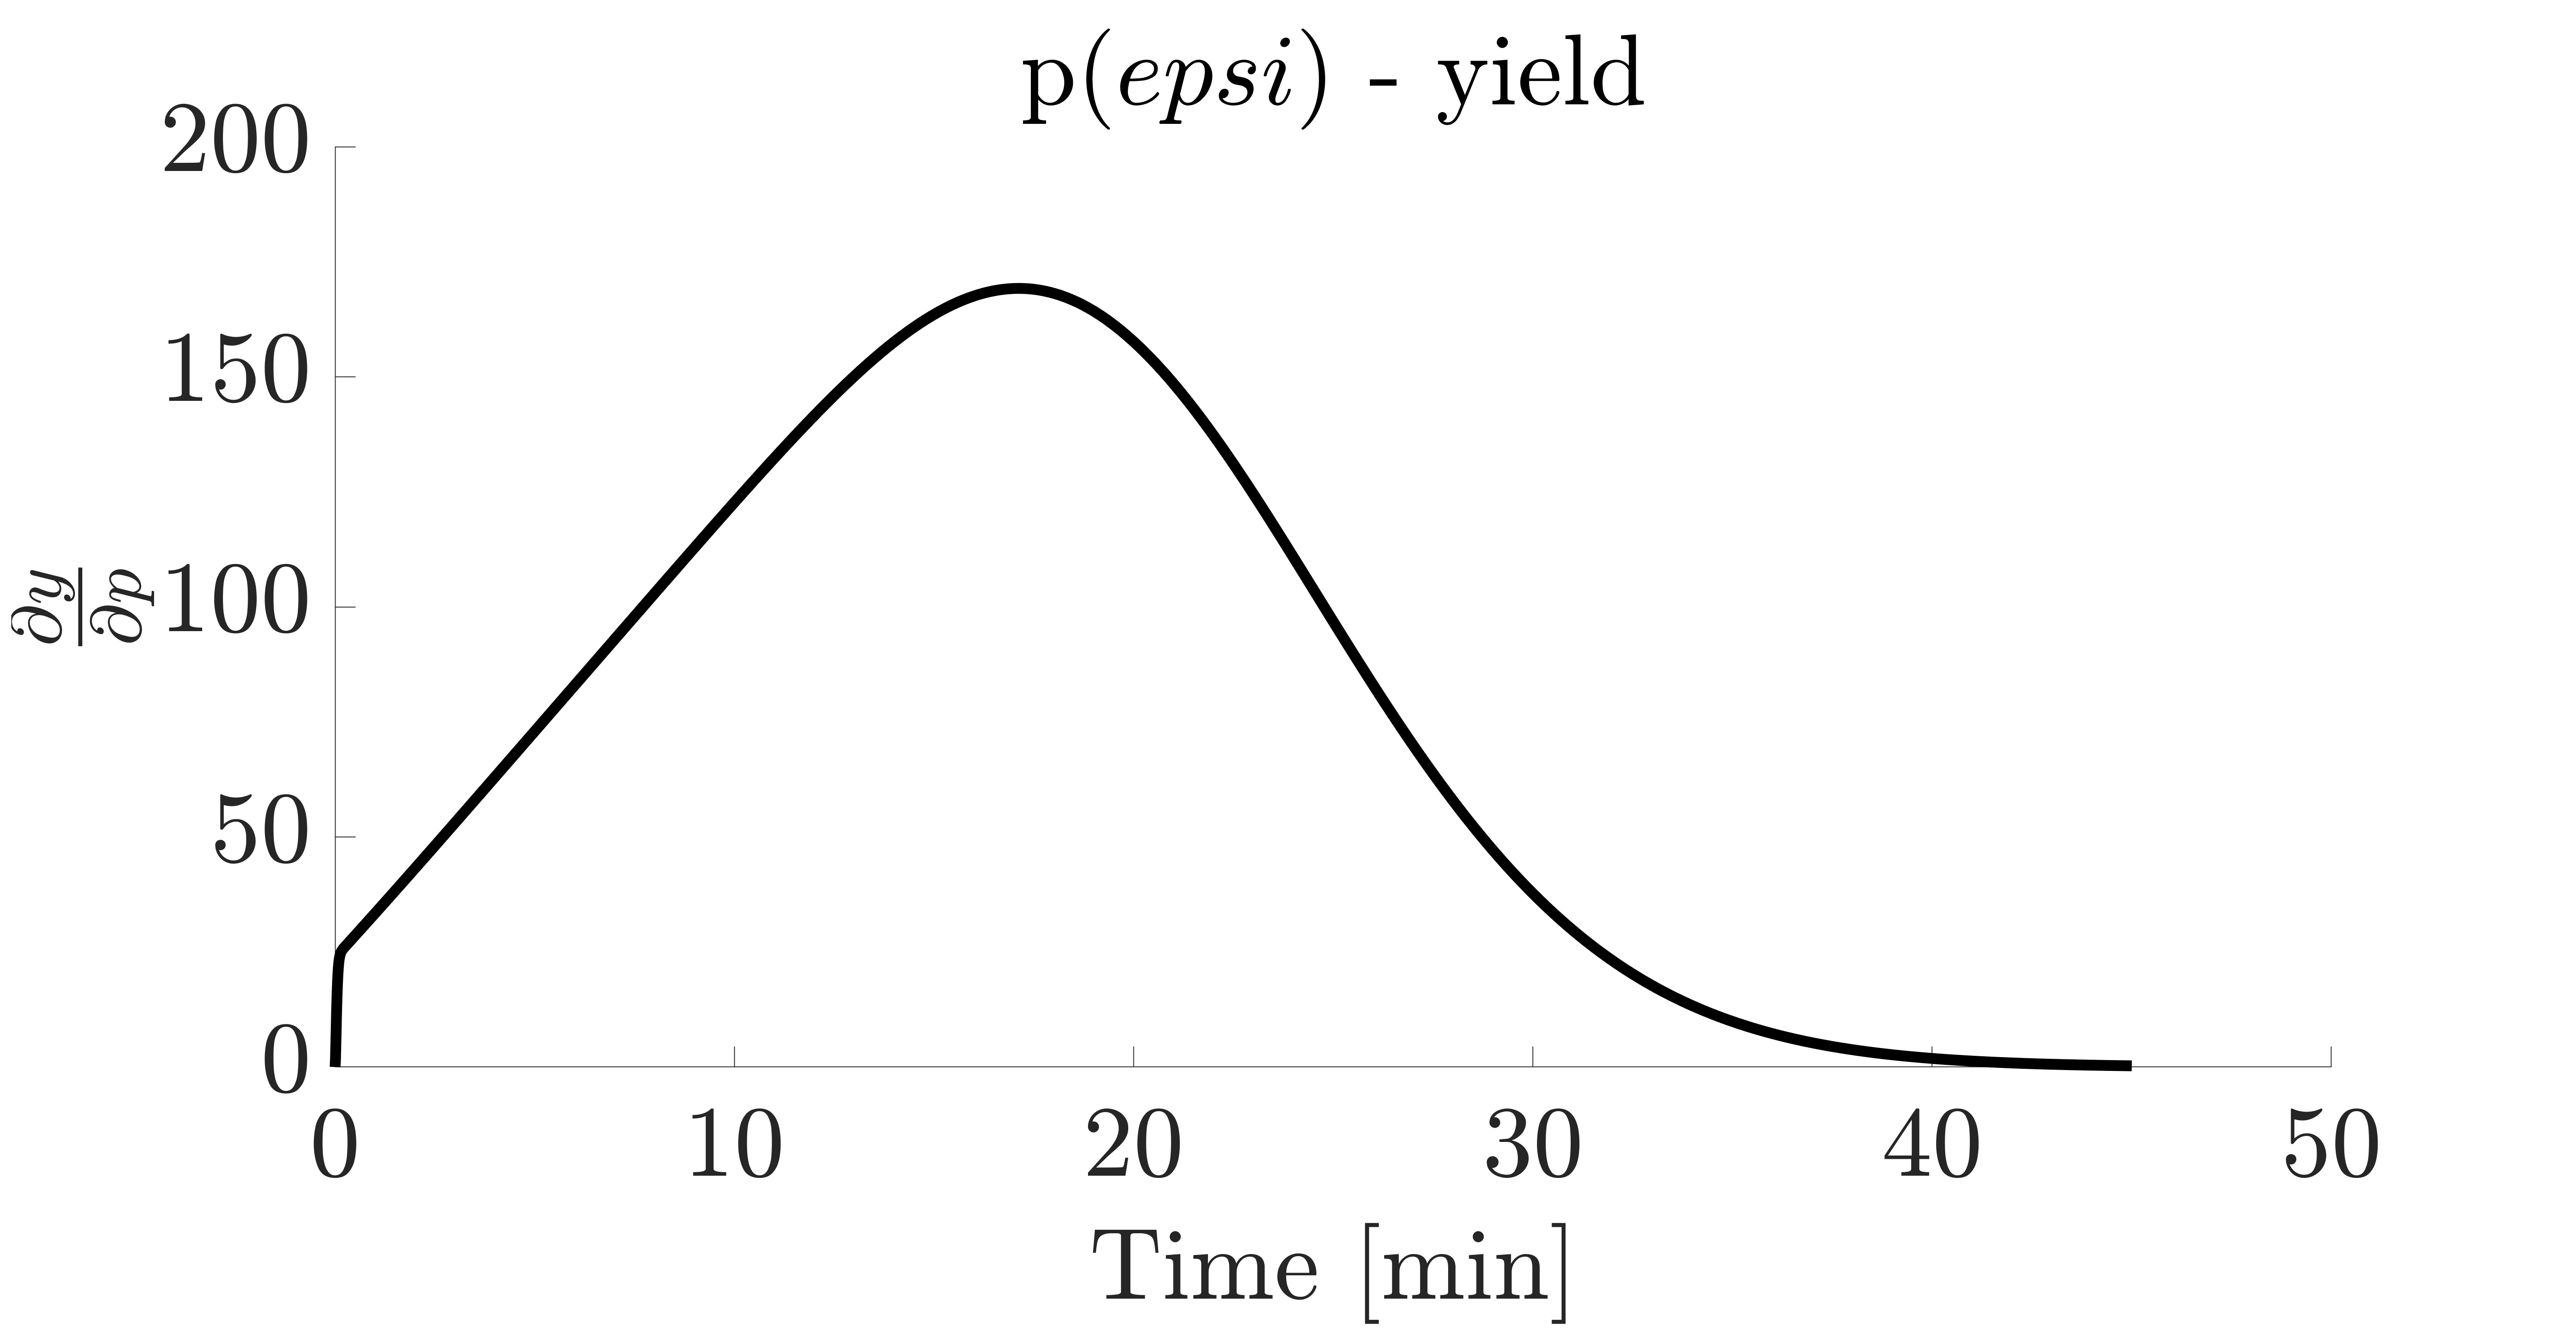
\includegraphics[width=5.5cm,height=2.5cm]{Figures/Sensitivity/Plots/1_SS_R_epsi.png}\\
		\end{columns}	
	\end{frame}

	\begin{frame}[fragile]{Sensitivity Analysis - Internal Diffusion}
	\tiny{
		\begin{align*}
			\cfrac{\partial \textcolor{blue}{c}(t,z)}{\partial t} &=  -\cfrac{F(t)}{\epsilon A\rho(T(t,z)P(t))} \cfrac{\partial c(t,z)}{\partial z} 
			+ D^M_e(T(t,z)P(t)) \cfrac{\partial^2 c(t,z)}{\partial z^2} + \cfrac{1-\epsilon}{\epsilon} \cfrac{\textcolor{orange}{D_i}(\textcolor{blue}{T}(t,z))}{\mu l^2 }\left(q(t,z) - \cfrac{c(t,z)\rho_s}{k_m(T(t,z))\rho(T(t,z)P(t))} \right)\\
			\cfrac{\partial \textcolor{blue}{q}(t,z)}{\partial t} &= -\cfrac{\textcolor{orange}{D_i}(\textcolor{blue}{T}(t,z))}{\mu l^2 }\left(q(t,z) - \cfrac{c(t,z) \rho_s}{k_m(T(t,z))\rho(T(t,z)P(t))} \right)\\
			\cfrac{\partial \textcolor{blue}{T}(t,z)}{\partial t} &= -\cfrac{F(t)}{A} \cfrac{C_p(T(t,z)P(t))}{ [(1-\epsilon)\rho(T(t,z)P(t)) C_p (T(t,z)P(t)) + \epsilon \rho_s C_{ps} ]} \cfrac{\partial T(t,z)}{\partial z} 
			+ D^T_e(T(t,z)P(t)) \cfrac{\partial^2 T(t,z)}{\partial z^2}
	\end{align*}}
	\begin{columns}[t]
		\column{.5\textwidth}
		\centering
		\includegraphics[width=5.5cm,height=2.5cm]{Figures/Sensitivity/Plots/2_SS_R_betah_{Di}.png}\\
		\includegraphics[width=5.5cm,height=2.5cm]{Figures/Sensitivity/Plots/3_SS_R_betah_{Di}.png}
		\column{.5\textwidth}
		\centering
		\includegraphics[width=5.5cm,height=2.5cm]{Figures/Sensitivity/Imagesc/2_SS_R_betah_{Di}.png}\\
		\includegraphics[width=5.5cm,height=2.5cm]{Figures/Sensitivity/Imagesc/3_SS_R_betah_{Di}.png}
	\end{columns}
\end{frame}

\begin{frame}[fragile]{Sensitivity Analysis - Internal Diffusion}	
	\tiny{
		\begin{align*}
			\cfrac{\partial \textcolor{blue}{c}(t,z)}{\partial t} &=  -\cfrac{F(t)}{\epsilon A\rho(T(t,z)P(t))} \cfrac{\partial c(t,z)}{\partial z} 
			+ D^M_e(T(t,z)P(t)) \cfrac{\partial^2 c(t,z)}{\partial z^2} + \cfrac{1-\epsilon}{\epsilon} 	\cfrac{\textcolor{orange}{D_i}(\textcolor{blue}{T}(t,z))}{\mu l^2 }\left(q(t,z) - \cfrac{c(t,z)\rho_s}{k_m(T(t,z))\rho(T(t,z)P(t))} \right)\\
			\cfrac{\partial \textcolor{blue}{q}(t,z)}{\partial t} &= -\cfrac{\textcolor{orange}{D_i}(\textcolor{blue}{T}(t,z))}{\mu l^2 }\left(q(t,z) - 	\cfrac{c(t,z) \rho_s}{k_m(T(t,z))\rho(T(t,z)P(t))} \right)\\
			\cfrac{\partial \textcolor{blue}{T}(t,z)}{\partial t} &= -\cfrac{F(t)}{A} \cfrac{C_p(T(t,z)P(t))}{ [(1-\epsilon)\rho(T(t,z)P(t)) C_p 	(T(t,z)P(t)) + \epsilon \rho_s C_{ps} ]} \cfrac{\partial T(t,z)}{\partial z} 
			+ D^T_e(T(t,z)P(t)) \cfrac{\partial^2 T(t,z)}{\partial z^2}\\
	\end{align*}}		
	\begin{columns}[t]
		\column{.5\textwidth}
		\centering
		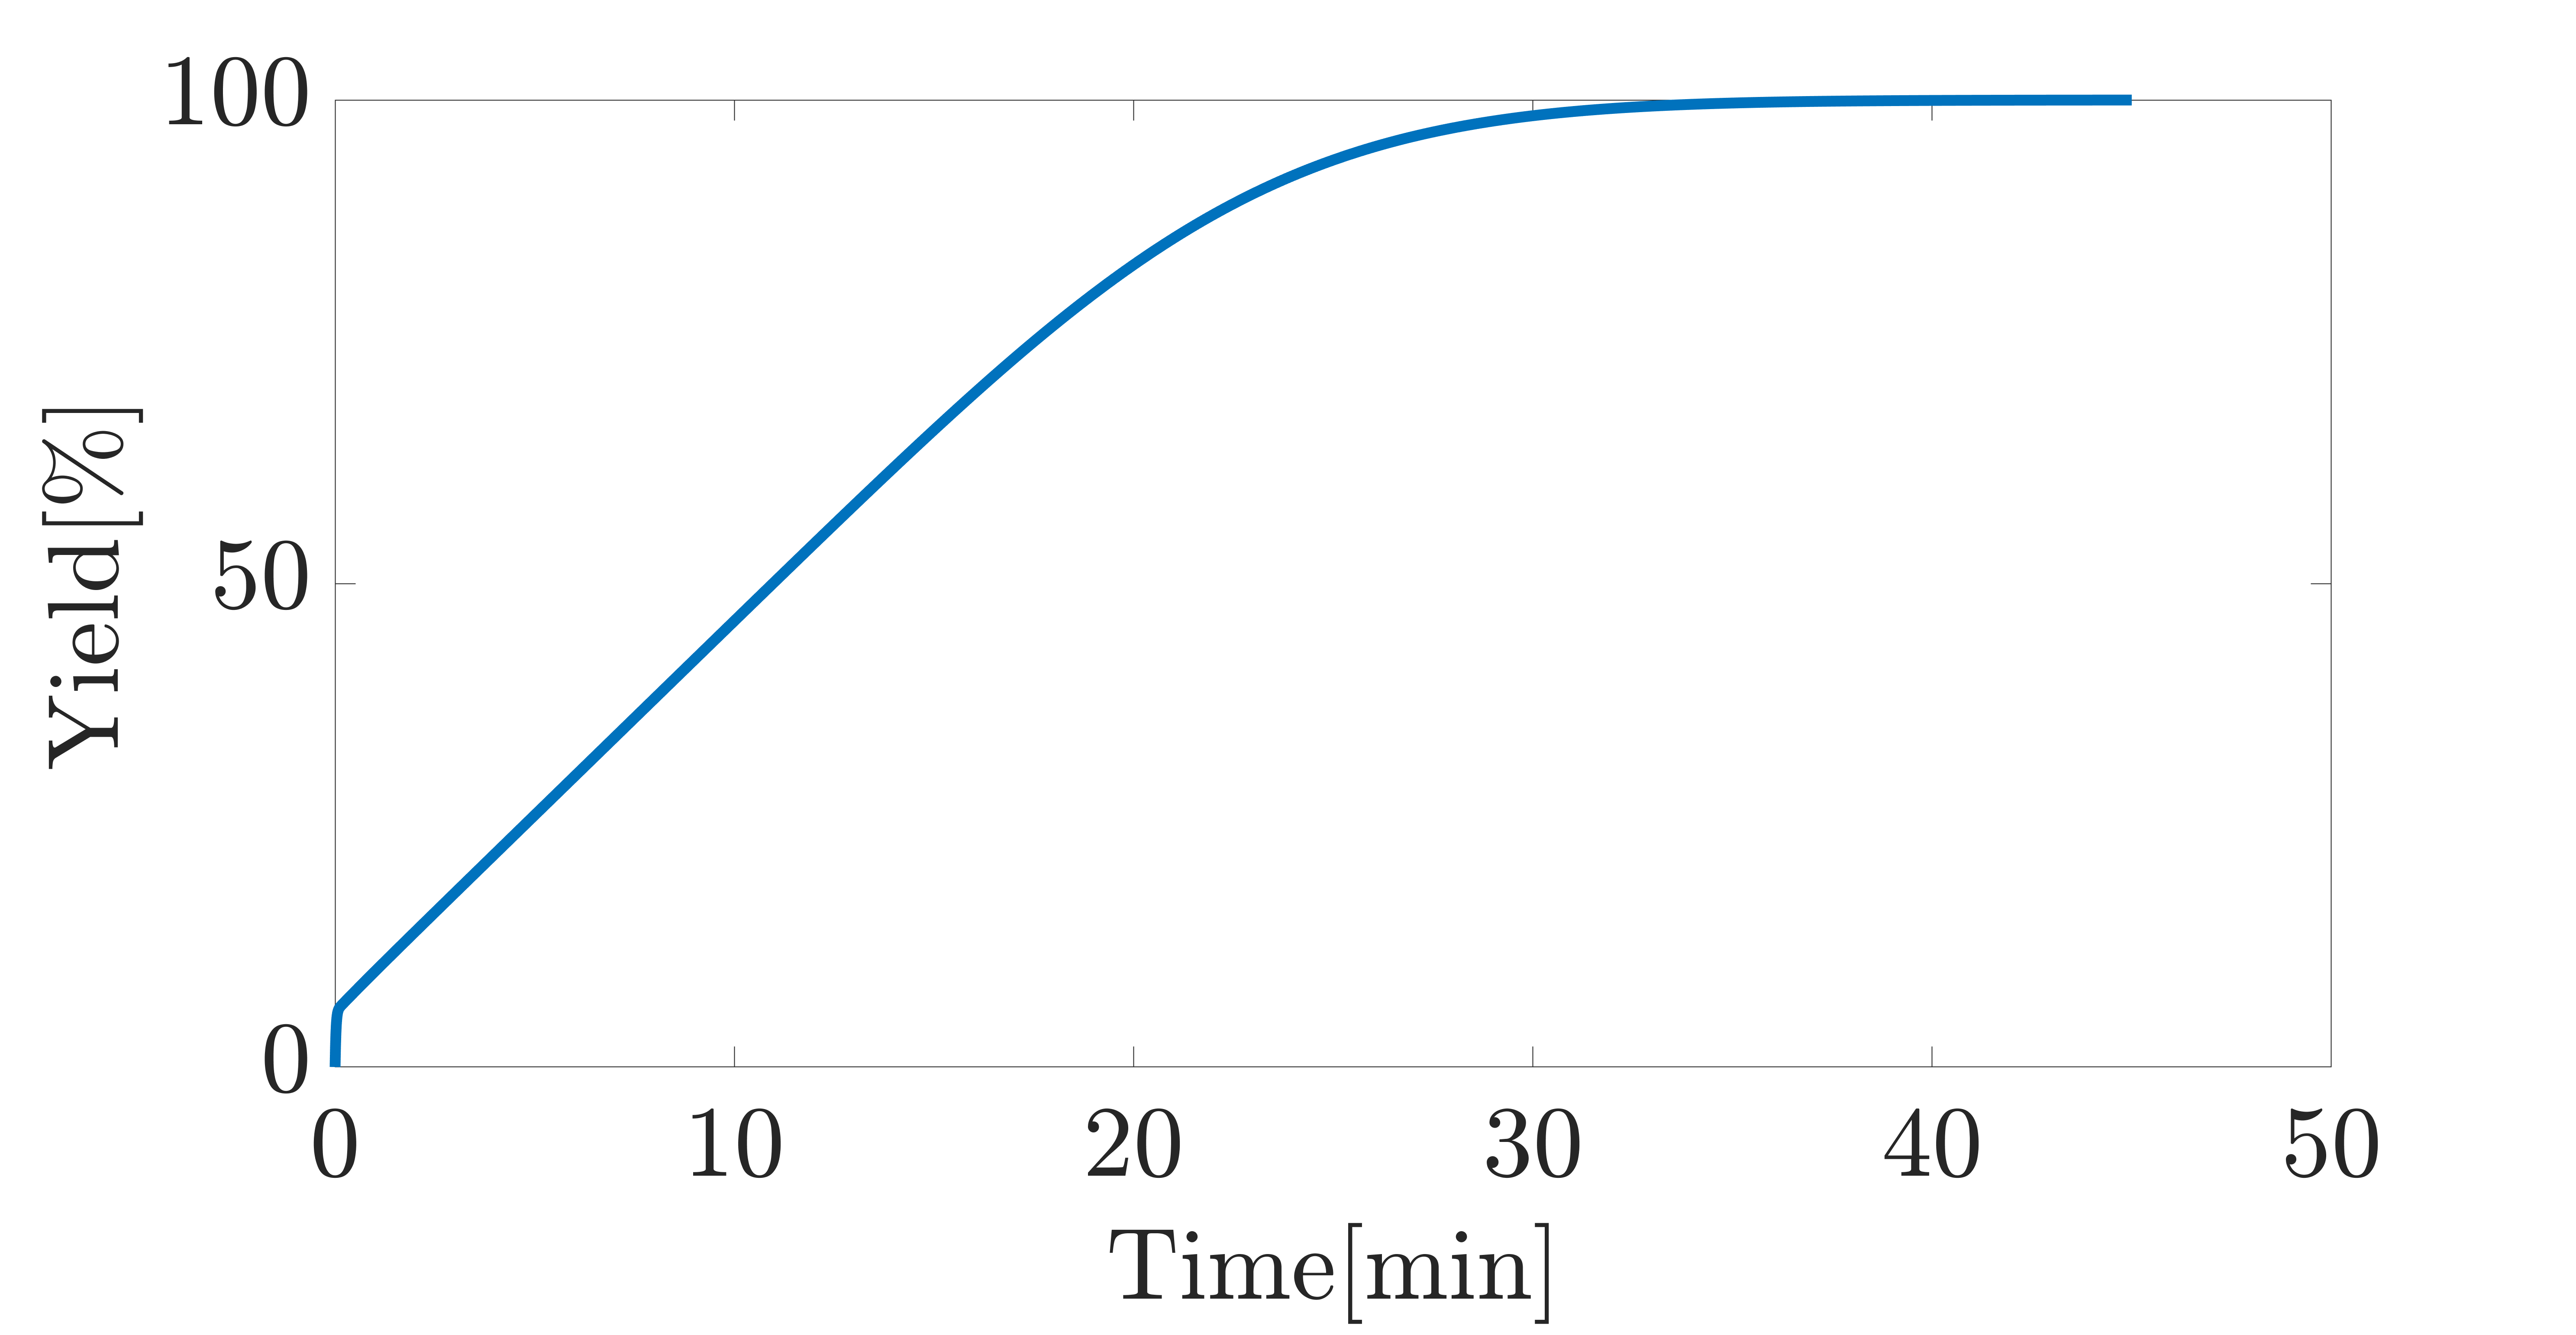
\includegraphics[width=5.5cm,height=2.5cm]{Figures/Sensitivity/Yield.png}\\
		\column{.5\textwidth}
		\centering
		\includegraphics[width=5.5cm,height=2.5cm]{Figures/Sensitivity/Plots/1_SS_R_betah_{Di}.png}\\
	\end{columns}	
	\end{frame}

	\begin{frame}[fragile]{What's next?}
		\begin{itemize}
			\item Paper related to the sensitivity analysis
			\item Control of the extraction process
			\item NovelBaltic
			\item Laboratory work 
		\end{itemize}
	\end{frame}
	
\end{document}
